\documentclass[a4paper,12pt,oneside,titlepage]{report}

\usepackage{listings} % evidenziazione codice
\usepackage{graphicx} % figure
\usepackage{url} % formattazione url
\usepackage{setspace} % interlinea
\usepackage[utf8]{inputenc} % lettere accentate in UTF-8
\usepackage{color}
\usepackage[]{frontespizio}
\usepackage{booktabs}
\usepackage{multirow}
\usepackage{subcaption}
\usepackage{float}
%\usepackage[parfill]{parskip}
%\usepackage[left=4cm,right=4cm,top=3cm,bottom=3cm]{geometry}

% Define colors
\definecolor{lgrey}{rgb}{0.95,0.95,0.95}
\definecolor{dblue}{rgb}{0,0,0.545}


\lstset{
	language=java,
	backgroundcolor=\color{white},
	basicstyle=\linespread{1.0}\ttfamily\small,
	%keywordstyle=\color{dblue}\bfseries,
	commentstyle=\color{black}\itshape,
	frame=tb,
	columns=fullflexible,
	showstringspaces=false,
	breaklines=true,
	numbers=left,%
    numberstyle={\tiny \color{black}},% size of the numbers
    numbersep=9pt % this defines how far the numbers are from the text
}

% Redefine \emph{} as bold
\let\emph\relax % there's no \RedeclareTextFontCommand
\DeclareTextFontCommand{\emph}{\bfseries}


\begin{document} 
%\pagenumbering{roman}
\onehalfspacing % interlinea 1.5
\nocite{*} % inserisce nella bibliografia fonti non citate

\begin{frontespizio}
\Istituzione{Universit\`a di Pisa}
\Dipartimento{Ingegneria dell'Informazione}
\Corso[Laurea Magistrale]{Computer Engineering}
\Titoletto{Tesi di Laurea Magistrale}
\Logo[2.0cm]{img/unipi_pdf.pdf}
\Rientro{1.0cm}
\Titolo{Enabling relay-based communication in LoRa\\
networks for the Internet of Things: design,\\
implementation and experimental evaluation
}
\Candidato[456615]{Alessio Sanfratello}
\Relatore{Prof.~Enzo Mingozzi}
\Relatore{Prof.~Francesco Marcelloni}
\Annoaccademico{2015/2016}
\end{frontespizio}

%\parskip = 2mm


\begin{flushright}
	\begin{minipage}{0.5\columnwidth}
		\begin{flushright}
			\textit{Ai miei genitori, che mi hanno sempre voluto bene}
			\\[1\baselineskip]
			\textit{A Margherita, che ha vissuto questa tesi in prima persona}
			\\[1\baselineskip]
			\textit{A Giacomo, Carlo e il prof. Mingozzi, che sono sempre stati pronti ad aiutarmi quando ne ho avuto bisogno}
			\\[1\baselineskip]
			\textit{Alla C3S, che se sono arrivato fin qui è anche grazie a loro}
			\\[1\baselineskip]
			\textit{Al MMAB e alle giornate passate più a cazzeggiare che a studiare}
			\\[1\baselineskip]
			\textit{Alla mia famiglia, ai miei amici e a tutti quelli che mi vogliono bene}
		\end{flushright}
	\end{minipage}
\end{flushright}




\chapter*{Abstract}

LPWANs have recently arisen as game changer in the field of the Internet of Things thanks to the wide coverage area, low cost of adoption and maintenance, and very low power consumption. Among the many incompatible technologies present on the market, LoRa seems to be the most promising one, combining good performance to an open specification of its MAC layer, called LoRaWAN. Because of these reasons LoRa immediately attracted the attention of both the scientific community and the industrial world, making it one of the most widely used LPWAN technology in the world. 

The aim of this work is to perform a deep and complete evaluation of the LoRa technology, exploring all the possibilities offered by the numerous parameters on which is possible to operate. To achieve a complete control of the network a brand new platform independent server infrastructure was developed from scratch, and it was designed to be at the same time lightweight and flexible for the experimental needs.

The first phase of experiments was conducted by exploring all possible, but reasonable, combination of data rate, transmission power and forward error correction levels. The analysis of the results leaded to the design of an extension of the LoRaWAN protocol to enable relay based communication. Finally, a new set of experiments was performed in order to prove the performance improvement compared to the standard LoRaWAN solution.



\tableofcontents
\listoffigures
\listoftables
\lstlistoflistings

\chapter{Introduction}

In the field of the Internet of Things the interest against new and more efficient communication methods has recently increased so that now all major players in the industry are involved in the development process of new communication protocols.

Among them, the Low-Power Wide Area Networks (LPWANs) seem to be the most promising family of technologies thanks the encouraging performances advertised by its developers. They typically combine very long range of coverage with an high energy efficiency, making them the enablers for an all new class of smart applications. In the past few years several companies have tried to develop its own protocol, with quite different results. SIGFOX, for instance, developed the homonym modulation technique, but other than sell their own technology to other manufacturers, they decided to propose themselves also as a network operator, selling both the technology and the network access to all potential customers.

On the contrary, Semtech decided to follow a radical different path with LoRa, their own modulation technique. As matter of fact, the company decided to keep the monopoly only on the production of the transceivers, making LoRa available for developers since the beginning. Moreover they decided to open up the specification of LoRaWAN, the MAC layer wich runs on top of LoRa.

Due to the fact that LoRa was introduced only few years ago, there are no exhaustive performance evaluation in different environmental conditions, since the only available experimental results are related to well defined use cases.

The goal of this thesis is to compensate for the lack of data by designing and performing a set of experiments with the aim to discover the optimal parameters which, in different scenarios, minimize both the packet error rate and the energy consumption.

From the analysis of results of the aforementioned experiments it turned out that the use of a relay based approach in some conditions would lead to big performance improvement in terms of number of correctly received packets, without sacrificing the energy efficiency. Consequently an extension to the LoRaWAN protocol has been designed enabling the possibility for an end-device to act as relay depending on the needs. To prove the performance enhancements expected from the analysis phase, a new set of experiments was conducted. 

Another justification to the development of a relay-based solution can be found in "Understanding the limits of LoRaWAN"\cite{lorawanlimits}: the authors tried to highlight the weaknesses of this technology and proposed either to transform LoRaWAN into a Time Division Access (TDMA) network and to design multi-hop solution in order to reduce both the number of collisions and the needed transmission power. This two proposals were both successfully implemented in this thesis.

\section{Structure of the thesis}
Chapter 2 makes an overview on the current technologies available for the internet of things, focusing on the new and promising Low-Power Wide Area Networks (LPWANs) and in particular on LoRa.

In chapter 3 the focus is shifted to LoRaWAN, the open MAC layer which works on top of LoRa, summarizing the main features and presenting the strengths of the protocol. Moreover, the server infrastructure, needed to manage a LoRaWAN network, is analyzed along with the message protocol used to make all components communicate.

Chapter 4 describes both the architecture and the implementation of the new server infrastructure which has been designed from scratch to be suitable for experimental purposes

Chapter 5 includes all the experiments performed in order to evaluate the LoRaWAN technology, highlighting the design choices and presenting all the results.

Chapter 6 presents the new protocol which is designed to enable relay based communications in LoRaWAN networks, along with the implementation on the server and on the motes. 

In Chapter 7 the performance improvement achieved is reported through the results of another set of experiments conducted with the new relay protocol.

Finally, chapter 8 presents the conclusions and some hints for future development of this work.

\chapter{Technology overview}

The \emph{Internet of Things} is a new communication paradigm which has recently arisen in the context of computer networks. It consists of extending Internet connectivity to physical devices, vehicles, buildings and other items, enabling them to collect and exchange data. There are many features that distinguish IoT from previous network architectures:

\begin{itemize}
\item \emph{Machine-to-Machine paradigm}: unlike the traditional internet applications, such as emails or web, in the IoT the devices can communicate without requiring human interaction. For instance some sensor can collect data and send them to a controller, which is responsible for managing some actuators. In this case all communications are triggered by the devices without human interaction;

\item \emph{Wireless communications}: the new applications enabled by the IoT often require large range of coverage, especially considering Smart Cities. Thus, combined with an increasing density of the smart devices, leads to the need to have only wireless communications in the IoT scenario;

\item \emph{Low power consumption}: in the IoT scenario devices are often battery powered, so one of the goals for protocols designed specifically for the IoT is to minimize power consumption;

\item \emph{Place and Play}: To achieve an ubiquitous coverage, the IoT devices must run out-of-the-box, without requiring any configuration;

\item \emph{Low cost}: all hardware used for the IoT must be simple such that can be massive produced at low cost.
\end{itemize}
Therefore, in order for the Internet of Things to quickly spread out, it is necessary to find a communication technology that is designed from the beginning to meet this requirements. To this aim in the following pages the main communication technologies are described and quickly analyzed. 

\section{Current technologies}
Before exploring the features of LoRa and the other LPWANs, a small survey on the current available technologies which enable IoT applications is presented, highlighting qualities and drawbacks of each one.

\subsection{IEEE 802.15.4}
The family of IEEE 802.15.4 based technologies includes many standards, such as ZeeBee and 6LoWPAN, and at the moment is used by the vast majority of the connected \emph{things} \cite{centenaro}. In general IEEE 802.15.4 solutions are very low cost and have low energy consumption, however the short range of coverage raises the need of complex multi-hop architectures, which can be difficult to develop and deploy.

\subsection{Wi-Fi}
Wi-Fi, which is the commercial name for the IEEE 802.11 family of communication standard, is one of the most widespread wireless technologies in the world, being on the market since 1997. Even if Wi-Fi represents the state of the art of Wireless LANs, for which it has been designed since the beginning, it not the ideal solution for the IoT because of the high power consumption and the small range of coverage. As a matter of fact, Wi-Fi is used for IoT only when the aforementioned limits are not relevant, for instance in some smart home and smart building applications.

To overcome these issues the Wi-Fi alliance has developed a new revision of the standard, the IEEE 802.11ah, which solves part of the problems and enables the communication in sub-GHZ bands, with theoretical performances suitable for the IoT needs.

\subsection{Cellular networks}
Cellular networks, with its long range of communication and its almost ubiquitous coverage, is the technology which is probably the closest one to the IoT needs. As a matter of fact it is currently used in contexts in which any other competitors are able to reach its performances. 

However the use of licensed frequencies involves operating costs are not negligible. Moreover, the high data rates that are offered to the connected end-devices leads to significant power consumption, which may become a great issue for battery power devices.

To address these issues a new revision of the current state of the art cellular technology, LTE-M, is expected to be released in the near future.

\section{Low-Power WANs}

Low-Power WAN (LPWAN) technologies are designed for machine-to-machine (M2M) networking environments. With decreased power requirements, longer range and lower cost than a mobile network, LPWANs are thought to enable a much wider range of M2M and Internet of Things applications, which have been constrained by budgets and power issues.

LPWAN data transfer rates are very low, as well as the power consumption of connected devices. LPWAN enables connectivity for networks of devices that require less bandwidth than what the standard home equipment provides. Furthermore, LPWANs can operate at a lower cost, with greater power efficiency. The networks can also support more devices over a larger coverage area than consumer mobile technologies and have better bi-directionality.

The need for a technology such as LPWAN is increasing in industrial IoT, civic and commercial applications. In these environments, the huge numbers of connected devices can only be supported if communications are efficient and power costs low.

In the past few years several LPWAN technologies were developed, and in the following paragraphs the most promising ones are presented.

\subsection{SIGFOX}

SIGFOX, the first LPWAN technology proposed in the IoT market, was founded in 2009 and has been growing very fast since then. The SIGFOX physical layer employs an Ultra Narrow Band (UNB) wireless modulation, while the network layer protocols are the “secret sauce” of the SIGFOX network and, as such, there exists basically no publicly available documentation. Indeed, the SIGFOX business model is that of an operator for IoT services, which hence does not need to open the specifications of its inner modules.

The first releases of the technology only supported uni-directional uplink communication, i.e., from the device towards the aggregator; however bi-directional communication is now supported. SIGFOX claims that each gateway can handle up to a million connected objects, with a coverage area of 30–50 km in rural areas and 3–10 km in urban areas. \cite{centenaro}


\subsection{Ingenu}

An emerging star in the landscape of LPWANs is Ingenu, a trademark of On-Ramp Wireless, a company headquartered in San Diego (USA). The company developed and owns the rights of the patented technology called Random Phase Multiple Access (RPMA), which is deployed in different networks. Conversely to the other LPWAN solutions, this technology works in the 2.4 GHz band but, thanks to a robust physical layer design, can still operate over long-range wireless links and under the most challenging RF environments.\cite{centenaro}

%\subsection{Weightless}


\subsection{LoRa}

LoRa is a proprietary spread spectrum modulation technique, which was initially developed by Semtech, and now is under the control of the LoRa Alliance. Unlike the other LPWAN technologies, LoRa is based on the chirp spread spectrum modulation, which makes it resistant against multipath fading and Doppler effect, and improves the receiver’s sensitivity. 

Very long range of communication can be achieved with LoRa thanks to the sub-GHz radio bands and very low data rates. The chip rate is equal to the programmed bandwidth (chip-per-second-per-Hertz) and can take values of 125, 250 or 500 kHz. Moreover, the spreading factor (SF) for a LoRa link may be varied depending on the communication distance and desired on-air time. Since the spreading codes for different SFs are orthogonal, the simultaneous transmission in the same frequency channel using different SFs is possible. \cite{lpwancoverage}

To drastically reduce the interference problems, LoRa includes different level of forward error correction codes, which can be varied depending on the environmental conditions.





\chapter{LoRaWAN}
\label{chap:lorawan}

This chapter describes the LoRaWAN network protocol which is optimized for battery-powered end-devices.

LoRaWAN networks typically are laid out in a star-of-stars topology in which gateways relay messages between end-devices and a central network server at the backend. Gateways are connected to the network server via standard IP connections while end-devices use single-hop LoRa or FSK communication to one or many gateways. All communication is generally bi-directional, although uplink communication from an end-device to the network server is expected to be the predominant traffic.

%LoRaWAN networks are organized in a star-of-stars topology, in which a central network server is in charge of managing all LoRa end-devices, receiving via standard IP connections

\begin{figure}[h!]
\centering
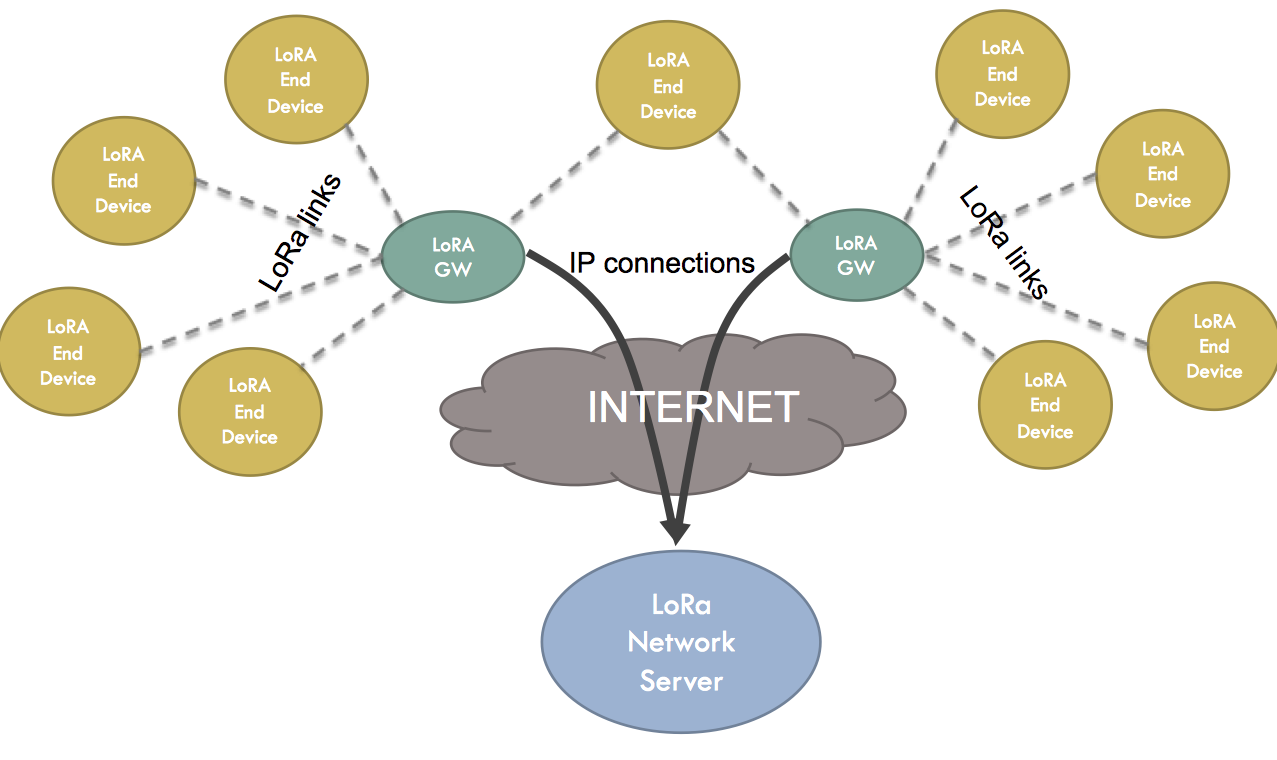
\includegraphics[width=\textwidth]{img/lora-arch}
\caption{Architecture}
\end{figure}

Communication between end-devices and gateways is spread out on different frequency channels and data rates. The selection of the data rate is a trade-off between communication range and message duration, communications with different data rates do not interfere with each other. LoRa data rates range from 0.3 kbps to 50 kbps. To maximize both battery life of the end-devices and overall network capacity, the LoRa network infrastructure can manage the data rate and RF output for each end-device individually by means of an adaptive data rate (ADR) scheme. \cite{lorawanspec}

\section{Specification}

\subsection{LoRaWAN classes}
LoRaWAN defines three classes of operation, of which only \emph{Class A} must be mandatorily implemented on all LoRaWAN compatible devices. Thanks to this policy we have a basic set of features which are present on all LoRaWAN end-devices, keeping both the architectural complexity and the production cost as low as possible.

In addition to the basic class, two more complex modes of operation has been defined with the aim to decouple downstream transmissions from the upstream ones. Given that these two advanced modes may be more expensive to design, produce and maintain, only end-devices who strongly requires these features are required to implement it.

\subsubsection{Class A: bi-directional end-devices}
In Class A communications each end-device's uplink transmission is followed by two short downlink receive windows. Each end-device schedules the transmission slots depending on its own needs, as in a ALOHA-type of protocol.

The main advantage of this communication scheme is the very low power consumption, while the biggest drawback is that this class of operation is suitable only for applications which allow to receive data only after the end-device has sent an uplink transmission. In fact downlink communications from the server at any other time will have to wait until the next scheduled uplink.


\subsubsection{Class B: bi-directional end-devices with scheduled receive slots}
In order to overcome the problem of non-deterministic latency on downlink communications, Class B increases the number of receive windows opened by the end-devices. These extra receive windows are synchronized with the server by means of a time-stamped beacon, which is broadcast by the gateway.


\subsubsection{Class C: bi-directional end-devices with maximal receive slots}
To offer the lowest possible latency to the server for downlink communication, Class C end-devices have a continuously open receive windows, which is closed only when transmitting data. This better performances are offered at the cost of an higher power consumption than Class A and B.

\subsection{Class A receive windows}
Following each uplink transmission the end-device opens two short receive windows. The receive window starts exactly after a predefined interval of time from the transmission of the last uplink bit. \cite{lorawanspec}

\begin{figure}[h!]
\centering
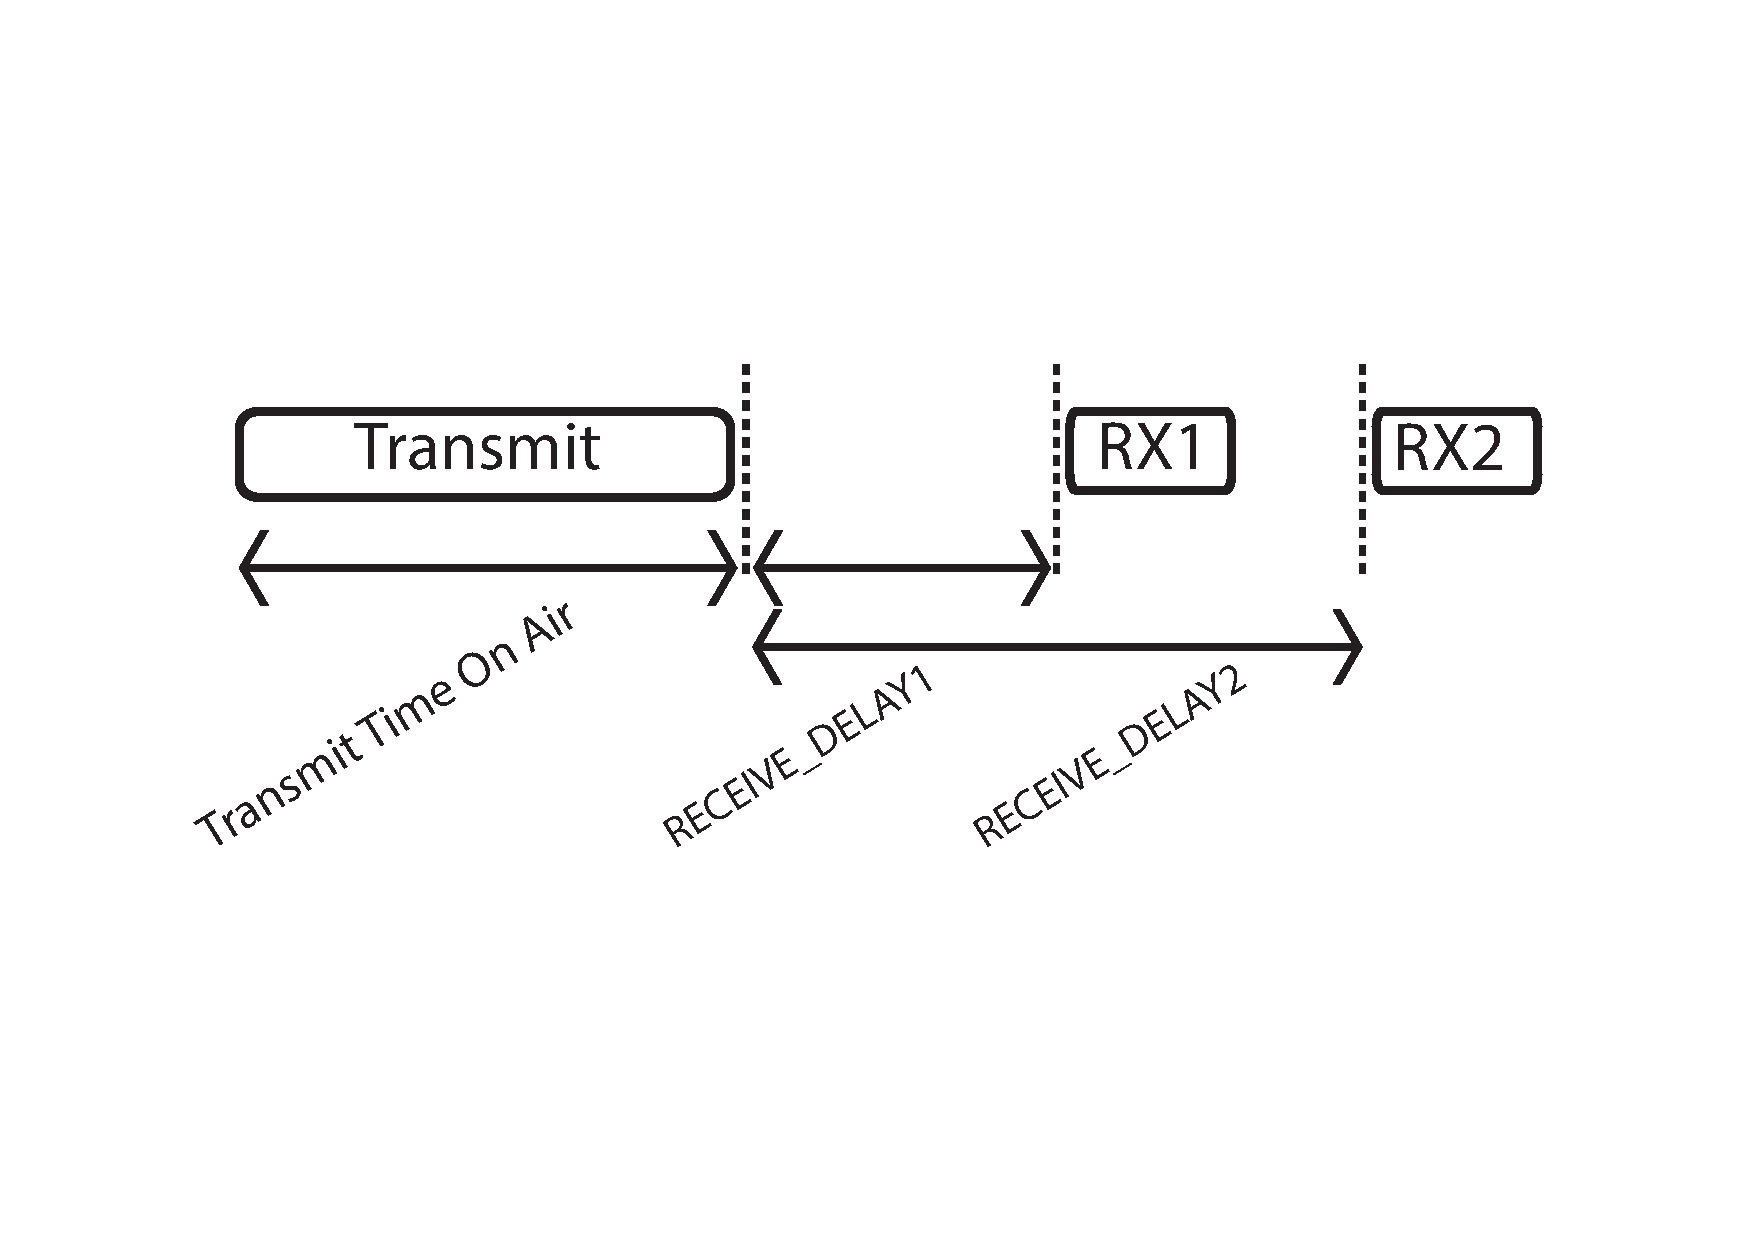
\includegraphics[width=\textwidth]{img/recwin}
\caption{LoRaWAN receive windows}
\end{figure}


The first receive window (RX1) is opened after RECEIVE\_DELAY1 milliseconds, which by default is set to 1 second. It uses the same frequency as the previous uplink transmission, and in general also the same data rate (in some regions may be a function of the uplink data rate).

The second receive window (RX2) is opened after RECEIVE\_DELAY2 milliseconds, which is defined as RECEIVE\_DELAY1 + 1 second. The frequency and the data rate are fixed for all transmissions, which means that they do not depend on the previous uplink communication, and they are configurable through a MAC command (table \ref{tab:cmd1}).

Each receive window is kept open at least for the time required to detect preamble of a LoRa downlink transmission, which is in the order of microseconds. If a frame is correctly received during the first receive window, the end-device does not open the second one. An end-device shall not transmit an other uplink message before a downlink message is received or the RX2 window is expired.


\subsection{Message Format}
LoRaWAN provides a full stack network protocol, having features of data-link, network and transport layer, and natively supporting encryption, authentication and reliable communication trough packet retransmission.

\subsubsection{Radio physical layer}

Each LoRa packet carries a physical payload (\emph{PHYPayload}) which contains LoRaWAN messages. When a LoRa packet contains a LoRaWAN message the CRC field, calculated on PHYPayload, is present only in up-link transmissions, since it is disabled for down-link transmissions.

\begin{figure}[h!]
\centering

\includegraphics[width=\textwidth]{img/msgformat/radio}
\caption{LoRa radio physical layer (CRC only uplink messages)}
\end{figure}


\subsubsection{Physical payload}

The physical payload contains three main fields:

\begin{itemize}

\item \emph{MAC Header}: specifies the \emph{Message Type} and the \emph{version} of LoRaWAN;

\item \emph{MAC Payload}: contains the LoRaWAN Frame;

\item \emph{MIC}: the Message Integrity Code, it is calculated as specified in RFC 4493 and it authenticates each message to the LoRa Network Server.

$MIC = aes128_cmac(NetSessionKey, B0 | msg) [0...3]$

\end{itemize}

\begin{figure}[h!]
\centering
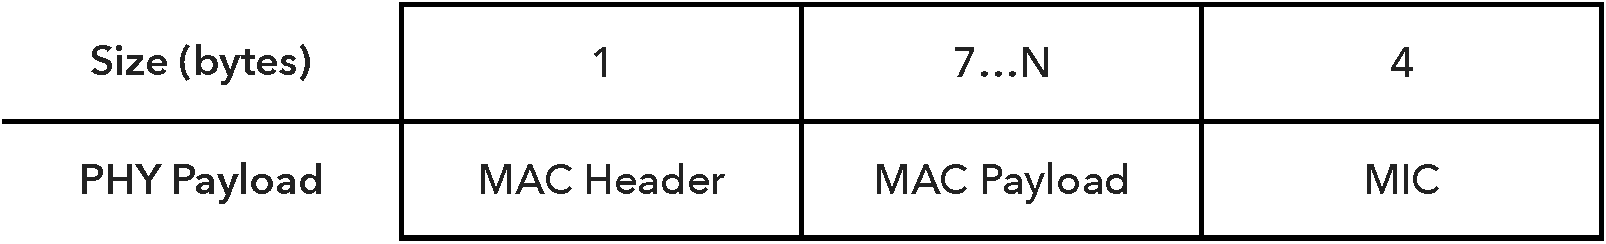
\includegraphics[width=\textwidth]{img/msgformat/phy_payload}
\caption{LoRa physical payload structured as a LoRaWAN message}
\end{figure}


\subsubsection{MAC Header}
The MAC header specifies the \emph{Message Type} and the \emph{version} of LoRaWAN. In table \ref{tab:msgtypes} all possible LoRaWAN message types are reported.


\begin{figure}[h!]
\centering
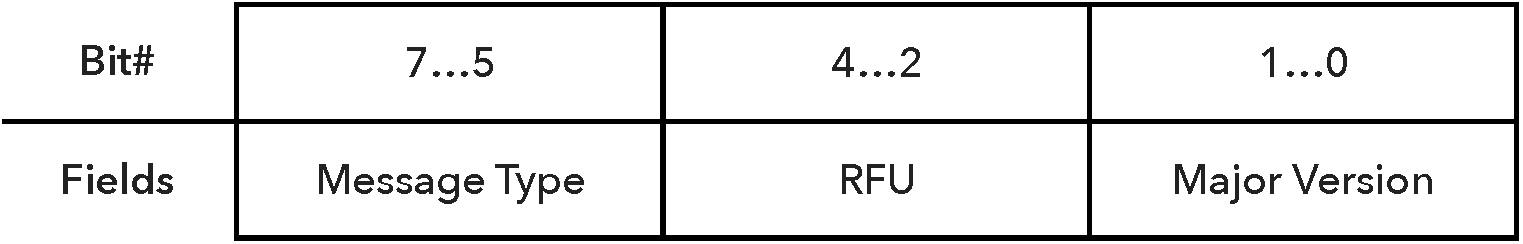
\includegraphics[width=\textwidth]{img/msgformat/mac_header}
\caption{LoRaWAN MAC header}
\end{figure}




% Please add the following required packages to your document preamble:
% \usepackage{booktabs}
\begin{table}[h!]
\centering
\caption{LoRaWAN message types}
\label{tab:msgtypes}
\begin{tabular}{@{}ll@{}}
\toprule
Msg Type & Description          \\ \midrule
000          & Join Request          \\
001          & Join Accept           \\
010          & Unconfirmed Data Up   \\
011          & Unconfirmed Data Down \\
100          & Confirmed Data Up     \\
101          & Confirmed Data Down   \\
110          & RFU                   \\
111          & Proprietary           \\ \bottomrule
\end{tabular}
\end{table}


\subsubsection{MAC Payload}
The MAC payload contains mandatory \emph{Frame Header} fields and optionally \emph{Frame Port} and \emph{Frame Payload}. Frame


\begin{figure}[h!]
\centering
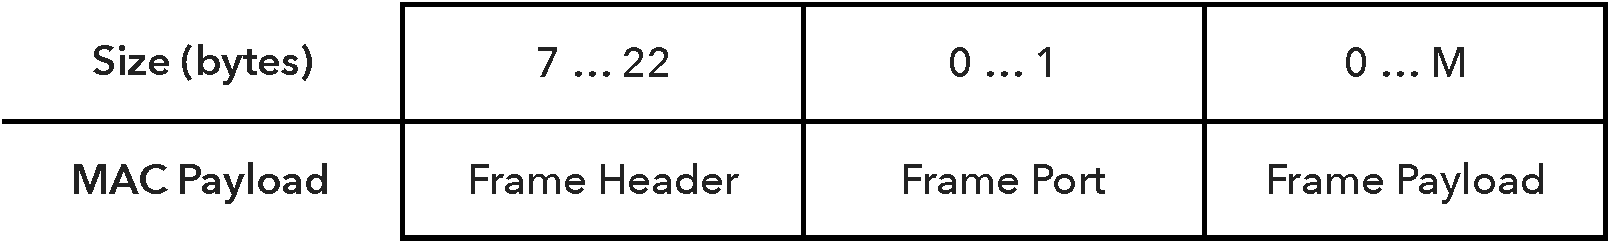
\includegraphics[width=\textwidth]{img/msgformat/mac_payload}
\caption{LoRaWAN MAC payload}
\end{figure}


\subsubsection{Frame Header}
The \emph{Frame Header} contains the 32 bit \emph{Device Address}, the \emph{Frame Control} field, the \emph{Frame Counter} and the \emph{Frame Options} field, which is used to piggyback MAC commands on user data traffic.

\begin{figure}[h!]
\centering
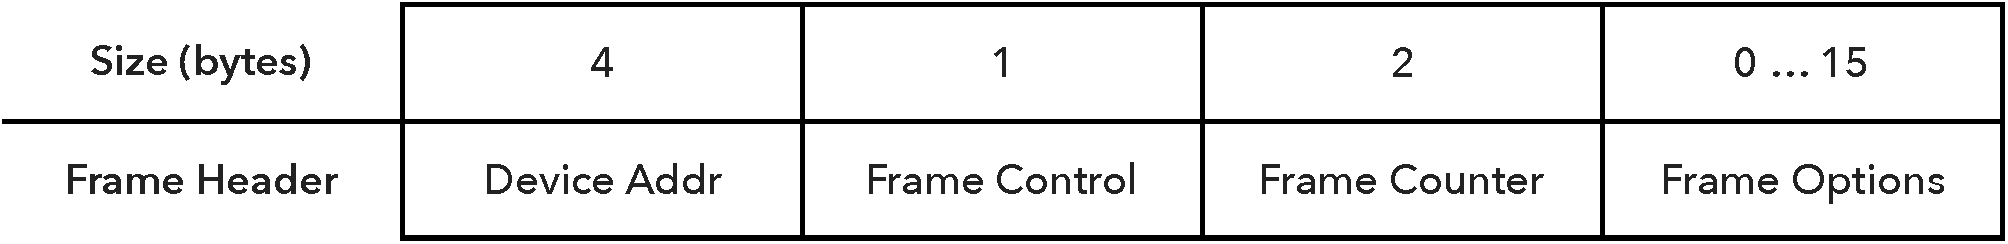
\includegraphics[width=\textwidth]{img/msgformat/frame_header}
\caption{LoRaWAN frame header}
\end{figure}

In the \emph{Frame Control} there are several important flags: the \emph{ADR} flag signals that data rate is controlled by network; the \emph{ADRACKReq} is set by the device to check if the gateway is still able to receive its traffic; the \emph{ACK} flag is set to acknowledge the previous received packet.

\begin{figure}[h!]
\centering
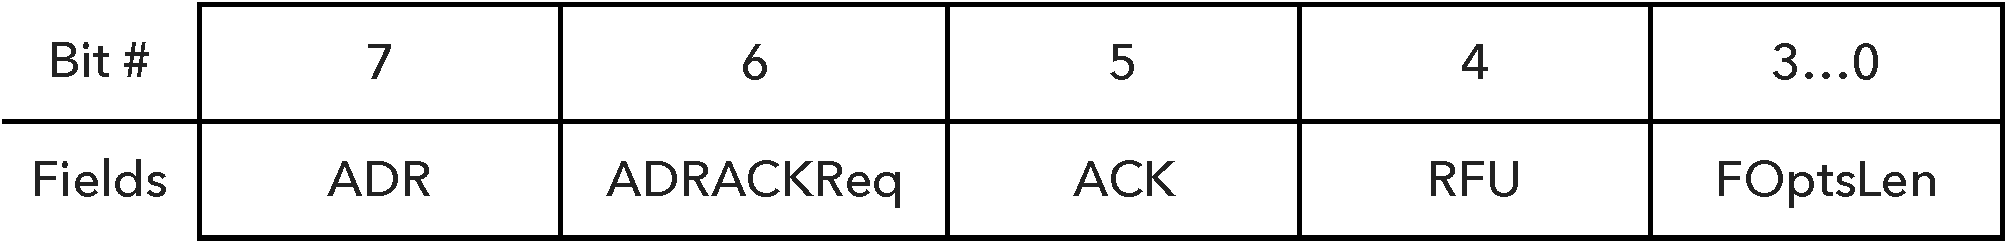
\includegraphics[width=\textwidth]{img/msgformat/frame_control}
\caption{LoRaWAN frame control}
\end{figure}


\subsubsection{Frame Port and Frame Payload}
By default LoRaWAN encrypts every Frame Payload by means of the \emph{Application Session Key}. If the Frame Payload carries a MAC command, then the Frame Port is set to 0 and it is encrypted with \emph{Network Session Key}.
If encryption is done above the LoRaWAN layer is possible to disable this features through a MAC command, but it is allowed only if the frame payload does not carry a MAC command itself.



\subsection{MAC Commands}
The MAC commands are a set of messages exchanged exclusively between the MAC layer of the end-devices and the network server. This messages may contain information useful for network administration purposes, such as checking the status of a device or changing some communication parameters, and they are never visible to the application server running in the cloud or the application running on the end-device.

MAC commands can be sent as Frame Payload, setting Frame Port to 0 and performing the encryption by means of the NetworkSessionKey. MAC commands can be also piggybacked in the FOpts field, and in this case they must not exceed 15 octets and they are sent always in clear.

A MAC command consists of a command identifier (CID) of 1 octet followed by a possibly empty command-specific sequence of octets. CIDs in the interval between 0x00 and 0x7F are reserved, while CIDs starting from 0x80 to 0xFF are available for proprietary network extensions.

Tables \ref{tab:cmd1} and \ref{tab:cmd2} contain the list of MAC commands defined in the LoRaWAN 1.0 specification.

% Please add the following required packages to your document preamble:
% \usepackage{multirow}
\begin{table}[]
\centering
\caption{MAC commands from 0x02 to 0x05}
\label{tab:cmd1}
\begin{tabular}{ccccl}
\hline
\multirow{2}{*}{CID} & \multirow{2}{*}{Command} & \multicolumn{2}{c}{TX by} & \multicolumn{1}{c}{\multirow{2}{*}{Description}}                                                                                                                                                       \\
                     &                          & ED               & GW              & \multicolumn{1}{c}{}                                                                                                                                                                                   \\ \hline
0x02                 & LinkCheckReq             & x                &                 & \begin{tabular}[c]{@{}l@{}}Used by an end-device to \\ validate its connectivity to\\ a network.\end{tabular}                                                                                          \\
0x02                 & LinkCheckAns             &                  & x               & \begin{tabular}[c]{@{}l@{}}Answer to LinkCheckReq\\ command. Contains the \\ received signal power\\ estimation indicating to the\\ end-device the quality of \\ reception (link margin).\end{tabular} \\
0x03                 & LinkADRReq               &                  & x               & \begin{tabular}[c]{@{}l@{}}Requests the end-device to \\ change data rate, transmit \\ power, repetition rate or\\ channel.\end{tabular}                                                               \\
0x03                 & LinkADRAns               & x                &                 & \begin{tabular}[c]{@{}l@{}}Acknowledges the \\ LinkRateReq.\end{tabular}                                                                                                                               \\
0x04                 & DutyCycleReq             &                  & x               & \begin{tabular}[c]{@{}l@{}}Sets the maximum \\ aggregated transmit duty-\\ cycle of a device\end{tabular}                                                                                              \\
0x04                 & DutyCycleAns             & x                &                 & \begin{tabular}[c]{@{}l@{}}Acknowledges a \\ DutyCycleReq command\end{tabular}                                                                                                                         \\
0x05                 & RXParamSetupReq          &                  & x               & \begin{tabular}[c]{@{}l@{}}Sets the reception slots \\ parameters\end{tabular}                                                                                                                         \\
0x05                 & RXParamSetupAns          & x                &                 & \begin{tabular}[c]{@{}l@{}}Acknowledges a \\ RXSetupReq command\end{tabular}                                                                                                                          
\end{tabular}
\end{table}



% Please add the following required packages to your document preamble:
% \usepackage{booktabs}
% \usepackage{multirow}
\begin{table}[]
\centering
\caption{MAC commands from 0x06 to 0xFF}
\label{tab:cmd2}
\begin{tabular}{@{}ccccl@{}}
\toprule
\multirow{2}{*}{CID}                                     & \multirow{2}{*}{Command} & \multicolumn{2}{c}{Transmitted by} & \multicolumn{1}{c}{\multirow{2}{*}{Description}}                                                                                            \\
                                                         &                          & ED               & GW              & \multicolumn{1}{c}{}                                                                                                                        \\ \midrule
0x06                                                     & DevStatusReq             &                  & x               & \begin{tabular}[c]{@{}l@{}}Requests the status of the \\ end-device\end{tabular}                                                            \\
0x06                                                     & DevStatusAns             & x                &                 & \begin{tabular}[c]{@{}l@{}}Returns the status of the \\ end-device, namely its \\ battery level and its \\ demodulation margin\end{tabular} \\
0x07                                                     & NewChannelReq            &                  & x               & \begin{tabular}[c]{@{}l@{}}Creates or modifies the \\ definition of a radio\\ channel\end{tabular}                                          \\
0x07                                                     & NewChannelAns            & x                &                 & \begin{tabular}[c]{@{}l@{}}Acknowledges a \\ NewChannelReq \\ command\end{tabular}                                                          \\
0x08                                                     & RXTimingSetupReq         &                  & x               & \begin{tabular}[c]{@{}l@{}}Sets the timing of the of \\ the reception slots\end{tabular}                                                    \\
0x08                                                     & RXTimingSetupAns         & x                &                 & \begin{tabular}[c]{@{}l@{}}Acknowledge \\ RXTimingSetupReq \\ command\end{tabular}                                                          \\
\begin{tabular}[c]{@{}c@{}}0x80\\ to\\ 0xFF\end{tabular} & Proprietary              & x                & x               & \begin{tabular}[c]{@{}l@{}}Reserved for proprietary \\ network command\\ extensions\end{tabular}                                            \\ \bottomrule
\end{tabular}
\end{table}



\subsection{End-device activation}
In order to participate in a LoRa network an end-device must obtain three information:
\begin{description}
\item[DevAddress] LoRa 32 bit address;
\item[NetSessionKey] 128 bit AES key, used for authentication;
\item[AppSessionKey] 128 bit AES key, used for encryption.
\end{description}
To this aim two possible join procedures exists: the \emph{Over-The-Air Activation} (OTA), in which each end-device must perform a join procedure involving the exchange of some messages with the server infrastructure, and the \emph{Activation by Personalization}, in which the end-devices already know the address and the keys, so they can bypass the join procedure.

While the activation-by-personalization may be trivially implemented by just load on all end-devices the address and the session keys, the OTA join requires both a protocol to get the information form the server, and an algorithm to generate the session keys.

The join procedure consists of two messages:
\begin{enumerate}
\item \emph{Join Request}, sent by the end-device to the server and containing \emph{AppEUI}, \emph{DevEUI} and \emph{DevNonce};
\item \emph{Join Accept}, sent by the server to the end-device and containing \emph{DevAddress}, \emph{NetID} and \emph{AppNonce}, all encrypted with a shared long-term \emph{AppKey}.
\end{enumerate}
If this procedure successfully completes, both the end-device and the server can run the key generation algorithm to compute the session key as described in \cite{lorawanspec}.


\subsection{Class B and Class C features}
Class B end-devices open receive windows, called \emph{ping slots}, at predictable time intervals, enabling server-initiated down-link messages, called \emph{ping}. To implement this feature all gateways must synchronously broadcast a beacon. If an end-device moves and detects a different beacon it must send an up-link message to update the routing path.

\begin{figure}[]
\centering
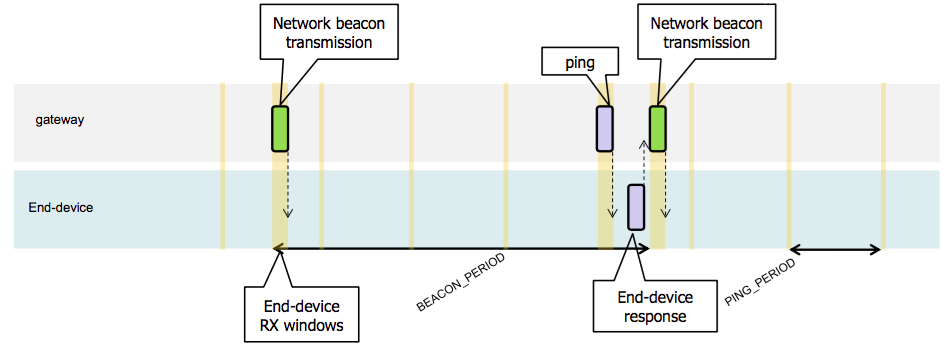
\includegraphics[width=\textwidth]{img/class_b}
\caption{Class B time diagram}
\label{fig:classb}
\end{figure}

All end-devices join the network as Class A, and the decision to switch to Class B must come from the end-device application layer. If so, the LoRaWAN layer searches for a beacon, and if it is found it selects the data rate and the periodicity of the ping slot.

The end-device must periodically transmit an uplink message to update the routing path in the network server. If no beacon is received for a period, it switches back to class A.

\begin{figure}[]
\centering
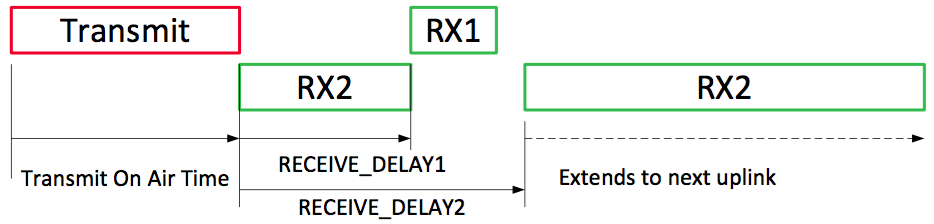
\includegraphics[width=\textwidth]{img/class_c}
\caption{Class C time diagram}
\label{fig:classc}
\end{figure}

Class C is implemented by opening RX2 as often as possible in order to be continuously listening to the channel. This leads to an inefficient protocol, with very high power consumption which is not suitable for battery powered end-devices. Class C end-devices cannot implement Class B option.

\subsubsection{Multicast}
In Class B and Class C mode devices may receive also multicast downlink frames. The \emph{multicast address}, the \emph{NetSessionKey} and the \emph{AppSessionKey} must come from the application layer and multicast frames are not allowed to carry MAC commands. Since ACK are not allowed while operating in multicast mode, the type of the LoRaWAN message must be “Unconfirmed Data Down”.



\section{GWMP: Gateway Message Protocol}
\label{sec:gwmp}
As already stated, each gateway communicates with the network server by means of a standard IP connection. Depending both on the network server and on the packet forwarder installed on the gateway, there can be used different application protocol.

The LoRaWAN specification does not require a specific gateway-to-server protocol, since the server needs to receive the complete LoRa physical payload, encapsulated in the most suitable protocol, depending on specific use case.

However Semtech, the company which has initially developed the LoRa modulation and the LoRaWAN protocol, released also its own gateway-to-server protocol, which is called \emph{Gateway Message Protocol} (GWMP).

GWMP relies on UDP, making it a connection-less protocol, and use the JSON format to carry the received frame with the associated statistics.

\subsection{Message format} Each GWMP message, as its shown in figure \ref{fig:gwmp}, includes three mandatory fields and two optional ones:
\begin{itemize}
\item \emph{Protocol Version}: the version of Gateway Message Protocol used;
\item \emph{Token}: number randomly chosen by the sender to uniquely identify the message;
\item \emph{Type}: it specifies the purpose of the message. Up to version 2 there are six different types defined;
\item \emph{Gateway EUI}: it contains the gateway identifier, based on the EUI-64 specification. It is not present in messages with types PUSH\_ACK or TX\_ACK;
\item \emph{Payload}: it contains a JSON formatted string;
\end{itemize}

\begin{figure}[]
\centering
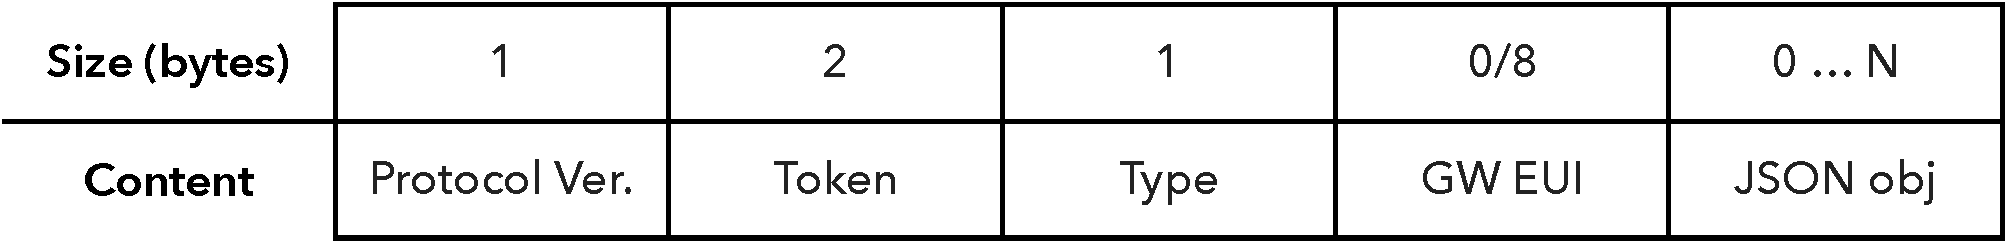
\includegraphics[width=\textwidth]{img/msgformat/gwmp}
\caption{GWMP packet format}
\label{fig:gwmp}
\end{figure}

\subsection{GWMP types}

\begin{itemize}
\item \emph{PUSH\_DATA}: used by the gateway to transmit the network server both the received LoRaWAN frames and other periodic statistics. Its total size shall not exceed 2408 octets;
\item \emph{PUSH\_ACK}: it is transmitted immediately by the network server on a receipt of a PUSH\_DATA message to acknowledge it. It does not contain the gateway EUI and the payload, and the token is the same of the PUSH\_DATA;
\item \emph{PULL\_DATA}: sent periodically by the gateway, it acts as a "keep alive" message informing the network server of the address and UDP port to which send any PULL\_RESP;
\item \emph{PULL\_ACK}: it is transmitted immediately by the network server on a receipt of a PULL\_DATA message to acknowledge it. It does not contain any payload and the token is the same of the PULL\_DATA;
\item \emph{PULL\_RESP}: carries in the JSON object the LoRaWAN frame to transmit to the end-devices and its size shall not exceed 1000 octets;
\item \emph{TX\_ACK}: present only in GWMP version 2, it is used by gateway to acknowledge a PULL\_RESP message.
\end{itemize}
Table \ref{tab:gwmptypes} summarizes all GWMP types;

\begin{table}[]
\centering
\caption{GWMP types}
\label{tab:gwmptypes}
\begin{tabular}{@{}cccc@{}}
\toprule
\multirow{2}{*}{Type} & \multirow{2}{*}{Code} & \multicolumn{2}{c}{Transmitted by} \\
                      &                       & Gateway      & Network Server      \\ \midrule
PUSH\_DATA            & 0x00                  & x            &                     \\
PUSH\_ACK             & 0x01                  &              & x                   \\
PULL\_DATA            & 0x02                  & x            &                     \\
PULL\_ACK             & 0x03                  &              & x                   \\
PULL\_RESP            & 0x04                  &              & x                   \\
TX\_ACK               & 0x05                  & x            &                     \\ \bottomrule
\end{tabular}
\end{table}



\subsection{GWMP Json protocol}
The Json object is used to carry the LoRaWAN messages and other information. To enhance compatibility only ASCII characters are allowed and there must be no white spaces outside the quoted text. Moreover, the top-level JSON object contains other objects as long as they respect the restriction explained above.

\subsubsection{Upstream transmissions}
In upstream transmissions the Json object may contain an array of RXPK objects, one for each LoRa message carried, and one STAT object, which carries some statistics on the gateway.

As already stated, each RXPK object contains a captured LoRa frame, which is encoded in the Base64 format, along with time of receipt and the information of the LoRa channel on which it was detected (data rate, coding rate, frequency, etc.). In listing \ref{list:rxpk} is shown an example of a possible RXPK object.

\begin{lstlisting}[caption={Example of an RXPK object}\label{list:rxpk}]
"rxpk":
[{
	"time":"2013-03-31T16:21:17.528002Z",
	"tmst":3512348611,
	"chan":2,
	"rfch":0,
	"freq":866.349812,
	"stat":1,
	"modu":"LORA",
	"datr":"SF7BW125",
	"codr":"4/6",
	"rssi":-35,
	"lsnr":5.1,
	"size":32, 
	"data":"-DS4CGaDCdG+48eJNM3Vai-zDpsR71Pn9CPA9uCON84"
}]
\end{lstlisting}
The STAT object is used to inform the network server of the status of the gateway. In particular it contains the geographical coordinates of the gateway and the statistics on received and forwarded message. An example of STAT object is reported in listing \ref{list:stat}.

\begin{lstlisting}[caption={Example of an STAT object}\label{list:stat}]
"stat":
{
	"time":"2014-01-12 08:59:28 GMT",
	"lati":46.24000,
	"long":3.25230,
	"alti":145,
	"rxnb":2,
	"rxok":2,
	"rxfw":2,
	"ackr":100.0,
	"dwnb":2, 
	"txnb":2
}
\end{lstlisting}

\subsubsection{Downstream transmissions}
The TXPK object is included in downstream messages to carry the downlink LoRa message along the needed information about the parameters, such as data rate, coding rate and frequency, to use for the transmission. It is important to remark that gateway, in general, do not have any notion about the LoRaWAN layer and its receive windows, so they rely on the time stamp included in the TXPK object to correctly synchronize themselves with the end-devices receive windows. Listing \ref{list:txpk} reports a possible instance of a TXPK object.
\\
\\
\begin{lstlisting}[caption={Example of an TXPK object}\label{list:txpk}]
"txpk":
{
	"imme":true,
	"freq":864.123456,
	"rfch":0,
	"powe":14,
	"modu":"LORA",
	"datr":"SF11BW125",
	"codr":"4/6",
	"ipol":false,
	"size":32,
	"data":"H3P3N2i9qc4yt7rK7ldqoeCVJGBybzPY5h1Dd7P7p8v"
}
\end{lstlisting}

\section{LoRa Servers}
\label{sec:loraservers}
\begin{figure}[]
\centering
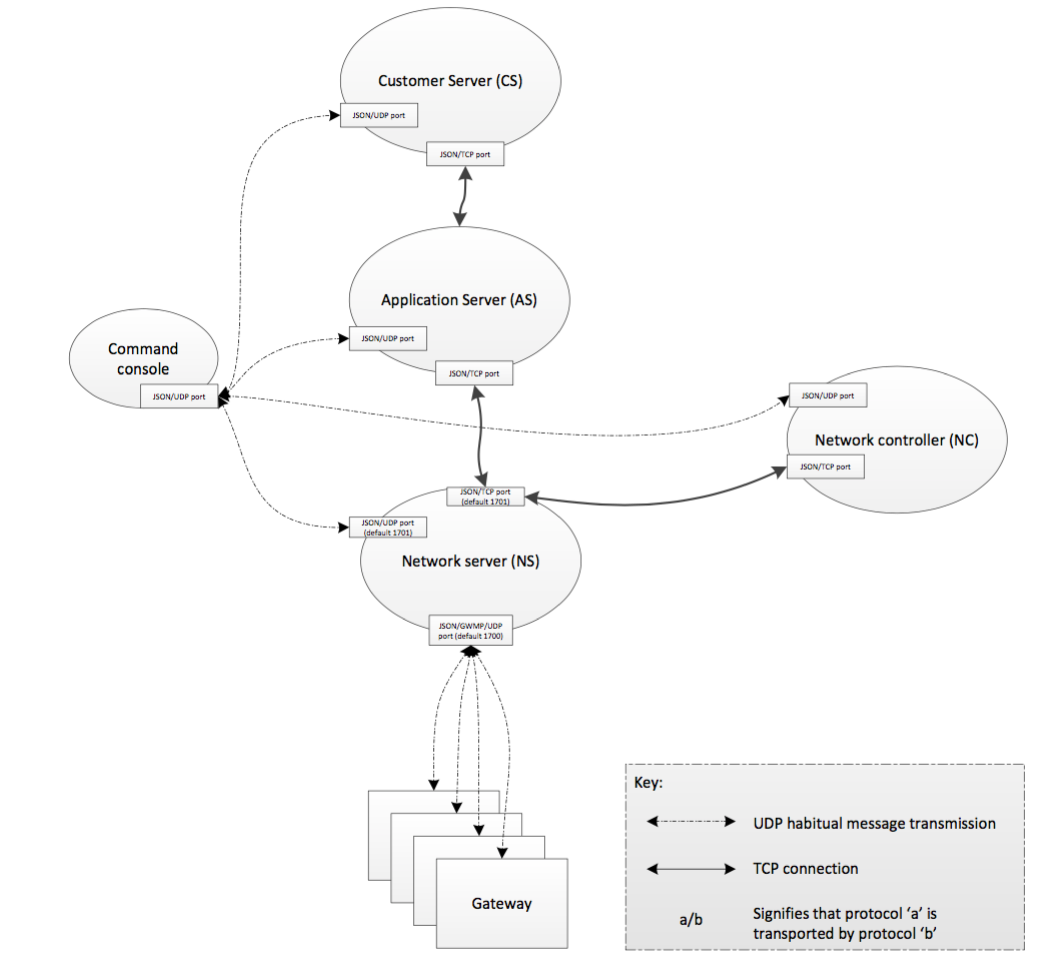
\includegraphics[width=\textwidth]{img/server_flow}
\caption{Architecture of the LoRa servers}
\end{figure}


In the LoRa architecture all the network management is done in the cloud by means of a set of servers. It consists of a \emph{Network Server}, which is responsible for all network management, one or more \emph{Application Server}, which are in charge of handling the end-device join and guarantee the secrecy of the communication. The Application Server may offer an interface to third party software, which in LoRa terminology is called \emph{Customer Server}.
Particularly important is the role played by the \emph{Network Controller}, which is in charge of managing the data rate and RF output for each end-device for which the adaptive data rate (ADR) scheme is enabled.

\subsection{Network Server}

The network server authenticates the received frame and forwards user data to an application server. The received frame is transported from the Gateway to the network server using JSON/GWMP/UDP/IP (defined in section \ref{sec:gwmp}). The frame is forwarded to an application server typically using JSON/TCP/IP.

The network server adds a cryptographic hash to all LoRa frames transmitted to the LoRa end-devices. The hash algorithm is defined by the LoRaWAN specification. \cite{lorawanspec}

A single network server may be connected to many application servers and network controllers. The remote server or controller used for a given mote is determined by the application to which the mote is assigned.

\subsection{Application Server}
The LoRa application server is responsible for admitting Over-The-Air end-devices to the network and for encrypting user data sent to, and decrypting user data received from, the end-device.
A single application server may be connected to many networks and customer servers. The remote server or controller used for a given mote is determined by the application to which the mote is assigned.
The LoRa application server decrypts the received user data and forwards it to a customer server. It also encrypts downstream user data before forwarding it to the network server. The encryption algorithm is defined by the LoRaWAN specification. \cite{lorawanspec}


\subsection{Network Controller}
The network controller receives the transmission parameters used by the mote and characteristics of the signal received by the gateway for each frame. It may perform operations using that data, for instance it may compute some statistics on it in order to find the optimal parameters that maximize the network capacity.
A single network controller may be connected to many network servers. The remote server or controller used for a given mote is determined by the application to which the mote is assigned.


\section{Related work}
The very good performances promised by LoRa, combined with the open specification of the MAC layer, attracted the attention of the scientific community on this technology. 

However the project started only few years ago, so there are not many detailed benchmarks on LoRa. In the following sections some works are reported.

\subsection{Free space measurament}
One of the first performance evaluation was performed in 2014 at the Offenburg University of Applied Sciences, Germany, by the Laboratory Embedded Systems and Communication Electronics. In their experiments they tried to find the maximum distance at which it is possible to transmit in the 868 MHz band with LoRa in free space and line-of-sight conditions.

Using the data rate SF10BW250 and coding rate 4/6 they were able to achieve 100\% of correctly received packets up to 7482 meters, when carrying 10 bytes of physical payload. Then they repeated the same experiment with 50 bytes of physical payload, achieving 94.1\% of correctly received packets at 6667 meters, and 80.33\% of correctly received packets at 7482 meters.\cite{freespace}


\subsection{2.4 GHz experiments for safety applications}
Other experiments were performed at the Offenburg University of Applied Sciences in 2015, focusing on the possible use of LoRa for safety applications. In all the four proposed scenarios only the 2.4 GHz band was tested.

In the first scenario they tried to find how many reinforced walls a LoRa packet could pass through, getting a promising result of 3 walls with 33\% of correctly received packets.

In the second scenario they proved that they need only one LoRa receiver to cover a floor, in comparison with Bluetooth LE which needs four receivers to cover the same area.

In the third scenario they achieved the 81.58\% of correctly received packets at 9.75 Km of distance in a true line-of-sight condition.

In the last scenario they tested the reliability of LoRa in salty water, obtaining 94.5\% of correctly received packets at 2 meters of distance in free space, plus 10 cm of salty water.\cite{safetylora}

\subsection{Wireless image sensor with shared activity time}
The main advantage of transmitting on ISM bands is that they are toll-free, while its disadvantage consists in the strict regulation on it. 

In particular, to overcome the duty cycle limit imposed on the 868 MHz band a french research team at the University of Pau, France, proposed to consider all the individual activity time in a shared/global manner, so that devices that need to go beyond the activity time limitation can borrow activity time from other devices.

This innovative proposal enables multimedia applications, such as image sensor for surveillance purposes, on the low bit rate LoRa network. To effectively share the activity time among the different devices they proposed through which the base station keeps track of the available \emph{Global Activity Time} and broadcasts it to all devices in its network.\cite{imagesensor}

\chapter{Design and implementation of a LoRa server}
\label{chap:server}

Since LoRaWAN was launched on the market a number of LoRa server has been released too. Most of them are presented as web services which provide the basic features of LoRaWAN for free, and in some case offering also some premium services. None of them, however, offers a complete control on the network, which is an essential requirement in order to completely explore the possibilities of this technology.

For these reasons it was decided to develop from scratch new LoRa server infrastructure, focusing in particular on designing a reliable tool which gives access to all information that can be extract from the behavior of the network. Moreover, having a complete custom software makes possible to make changes depending on the needs.

The goal of this work was to obtain a simple, yet flexible, software that can be adapted to different experimental condition without the of re-engineering a complex architecture. In other words, the solution which is presented in this chapter is not designed to be a competitor of the existing commercial network server.


\section{Architecture}
As is shown in figure \ref{fig:servercomponent}, the \emph{network server} and the \emph{application server} were designed to be two separate components, communicating through sockets. This choice follows the guidelines provided by Semtech, which are presented in section \ref{sec:loraservers}. Moreover, decoupling the two components makes possible to run them in different machines.

The communication with the gateway is done using the GWMP protocol presented in chapter \ref{chap:lorawan}, which makes this server immediately compatible with the majority of gateway present on the market.

\begin{figure}[]
\centering
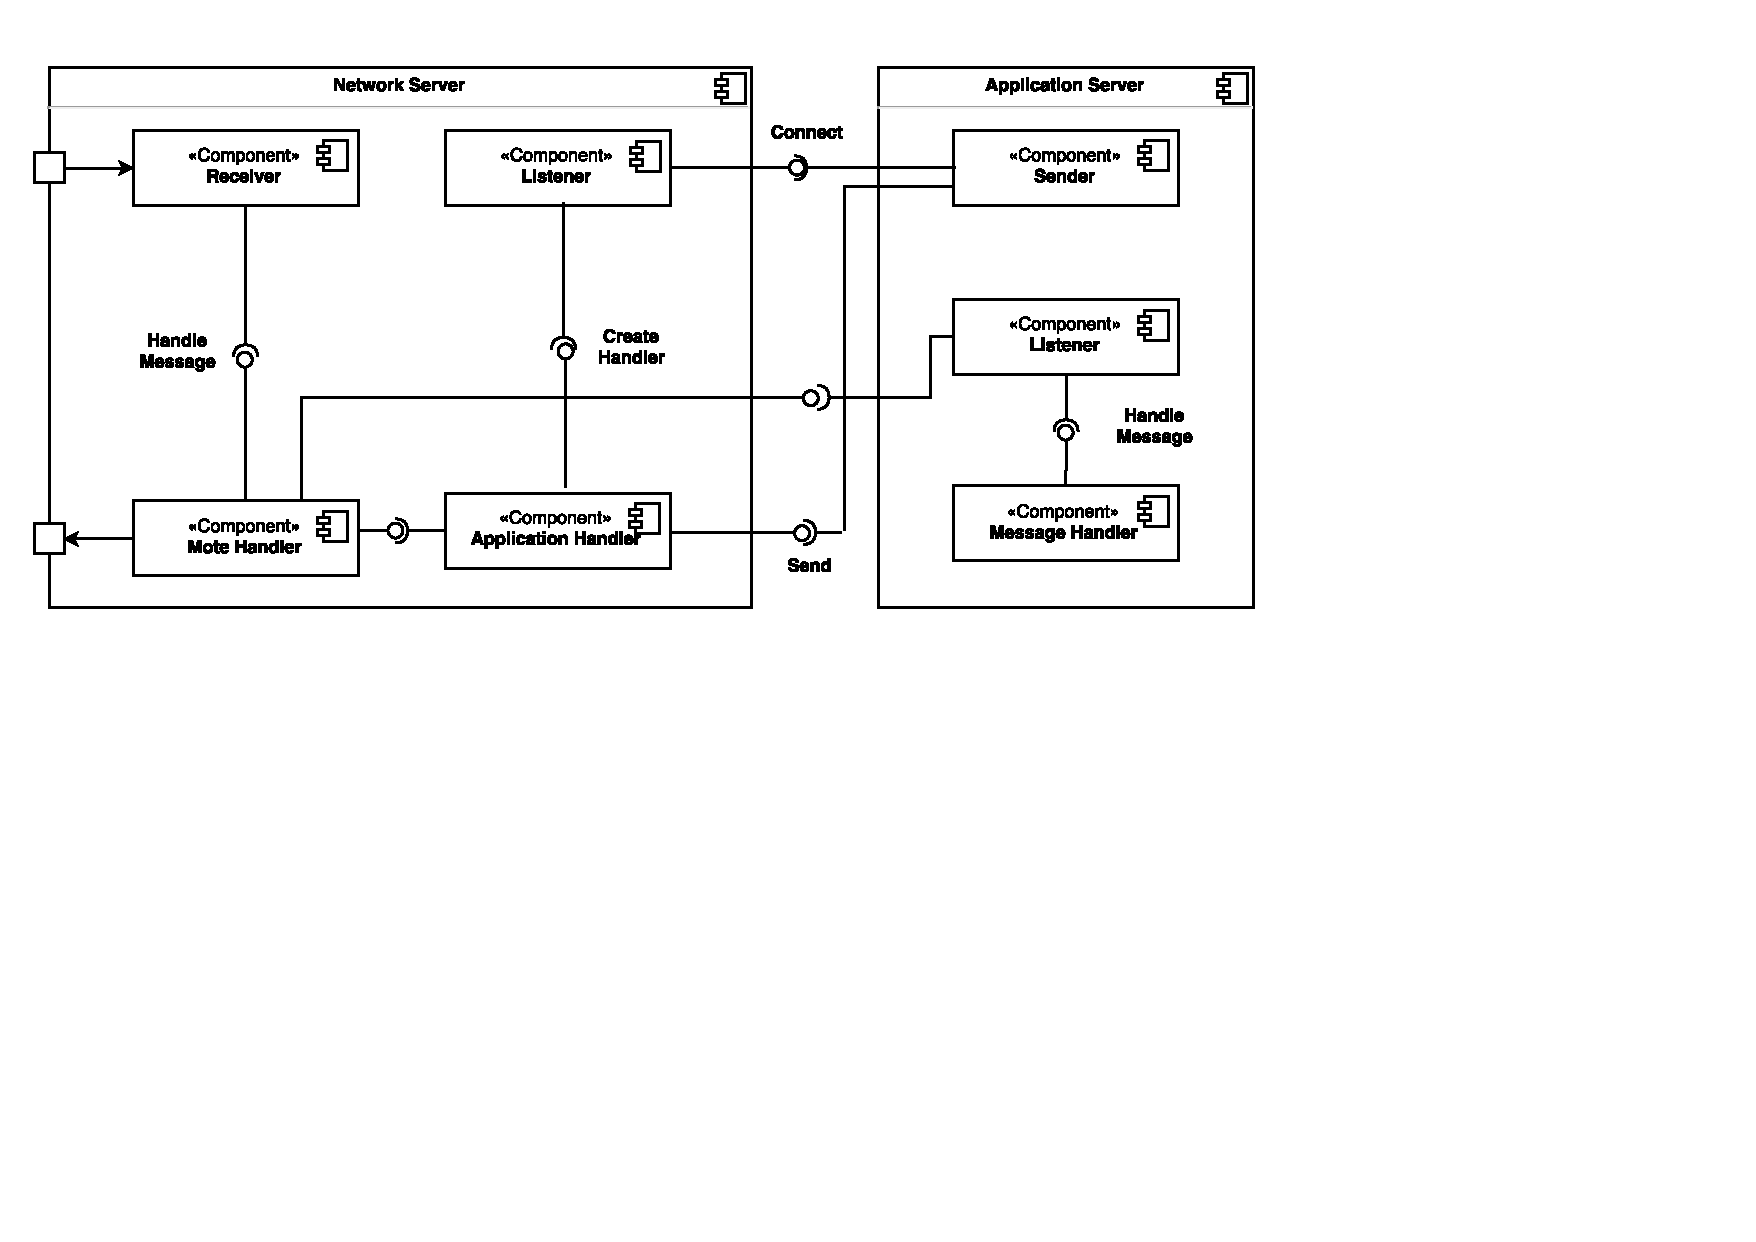
\includegraphics[width=\textwidth]{img/netserver}
\caption{Architecture of the network server}
\label{fig:servercomponent}
\end{figure}

\section{Network Server}
The network server consists of four separate components (figure \ref{fig:servercomponent}) which communicates among them by means of a set of shared data structure.

\subsubsection{Receiver}
The receiver component is responsible for receiving data from gateways trough to an UDP socket. If it receives a PULL\_DATA message, it stores address and port of the gateway in a dedicated data structure. In case of PUSH\_DATA, instead, it delivers the message to a pool of Mote Handler.

\subsubsection{Mote Handler}
The Mote Handler is charge of handling the message on a separate thread performing the following operations:

\begin{itemize}
\item it authenticates the frame by checking the MIC, and in case of failure it discards the message and terminates the execution;
\item it checks if the application server associated to the mote is connected to the network server and it forwards the user data to it;
\item it checks if there is a pending message to be sent to the mote; if the mote requested an acknowledgement by means of a \emph{Confirmed Data Up} message and there are no pending data, it sends back an empty message setting the ACK flag;
\item it updates the statistics of the correctly received message from the mote.
\end{itemize}


\subsubsection{Listener}
It waits for Application Servers that want to connect and creates an Application Handler for each one.

\subsubsection{Application Handler}
The Application Handler is responsible for receiving user data from the application server to which it is connected, and it pushes every received message to the pending queue of the corresponding mote.

\subsection{Implementation}
To obtain a platform independent product it was decided to implement it using the Java programming language, and in particular the Java 8 SDK. Since stability and reliability was a primary requirement the Network Server is implemented in a multi-thread fashion, so that every message is handled in a different thread. This choice brings greater robustness especially in unexpected situations because a wrong management of the message does not involve the malfunction of the entire server.

This multi-thread design is implemented by meas of the Java ExecutorService, in which a fixed pool of threads is created at start up and reused at run time.

In listing \ref{list:motehandler} the main function of each Mote Handler is shown. All data is stored in thread-safe data structures.

The Listener components implements the GWMP protocol to exchange data with gateways, while the MoteHandler parses uplink data and builds downlink messages on the basis of the LoRaWAN 1.0 specification.\cite{lorawanspec}

\begin{lstlisting}[caption=Main function of NetworkServerMoteHandler.java\label{list:motehandler}]
public void run() {
    if (message.getInt("stat") != 1) {
        activity.warning("CRC not valid, skip packet");
        return;
    }

    Packet packet = new Packet(message.getString("data"));

    switch (packet.type) {
        case Packet.JOIN_REQUEST:
            handleJoin(packet);
            break;
        case Packet.CONFIRMED_DATA_UP:
        case Packet.UNCONFIRMED_DATA_UP:
            handleMessage(packet);
            break;
        default:
            activity.warning("Message type not recognized");
    }
}
\end{lstlisting}
The most important function of the Mote Handler is the \texttt{handleMessage()}, reported in \ref{list:handlemsg}, which is in charge of handling the received packets, authenticating them and forwarding them to the Application Server. Since in class A LoRaWAN end-devices the receive windows are opened shortly after the upstream transmission, the first of which with the same parameters, the Mote Handler component must be responsible also for the correct transmission of the downstream messages. This operation is done in the \texttt{handleMessage()} by polling a frame from the queue of pending messages, and sending it to the gateway by means of the GWMP protocol.

\begin{lstlisting}[caption=Handle message in NetworkServerMoteHandler.java\label{list:handlemsg}]
private void handleMessage(Packet packet) {
    long timestamp = message.getLong("tmst");
    Frame fm = new Frame(packet);
    Mote mote = motes.get(fm.getDevAddress());

    if (mote == null) {
        activity.warning(fm.getDevAddress() + ": Mote not found");
        return;
    }

    // Authentication => check mic
    if (!packet.checkIntegrity(mote,fm.counter)) {
        activity.warning(fm.getDevAddress() + ": MIC not valid");
        return;
    }

    // Forward message to Application Server
    AppServer appServer = appServers.get(mote.getAppEUI());

    if (appServer == null) {
        activity.warning("App server NOT found");
    } else {
        String appserverMessage = buildAppserverMessage(gateway,message,packet.type,fm);
        try(Socket toAS = new Socket(appServer.address, appServer.port)) {
            PrintWriter out = new PrintWriter(new OutputStreamWriter(toAS.getOutputStream(), StandardCharsets.US_ASCII));
            out.println(appserverMessage);
            out.flush();
        } catch (IOException e) {
            e.printStackTrace();
        }
    }

    mote.updateStatistics(fm.counter); // Update mote statistics
    activity.info(mote.printStatistics());

    /*** SEND DOWNSTREAM MESSAGE ***/
    // Wait message to send
    String answer;
    try {
        answer = mote.messages.poll(TIMEOUT, TimeUnit.MILLISECONDS);
    } catch (InterruptedException e) {
        e.printStackTrace();
        return;
    }
    
    if (answer == null) {
        activity.info("Timeout, no message in queue to send to " + mote.getDevAddress());
        return;
    }

    Packet ansPacket = buildDownstreamMessage(answer, mote, (packet.type == Packet.CONFIRMED_DATA_UP));

    // If there there is one message in queue, send it
    GatewayMessage response = /* build response */
    try {
        socket.send(response.getPacket(gatewayAddr));
        activity.info("Sent message to mote: " + mote.getDevAddress());
    } catch (IOException e) {
        e.printStackTrace();
    }
}
\end{lstlisting}

\newpage
\section{Application Server}
The \emph{Application Server} includes three main components, as described by the component diagram in figure \ref{fig:servercomponent}.

\subsubsection{Sender}
The \emph{Sender} component is in charge of encrypt user data by means of the Application Session Key and it sends it to the Network Server. This component, and in general the overall application server, has no information on the timing constraint of the mote, so it sends the downstream message as soon they are produced. The correct scheduling of the messages into the correct receive window is done by the network server.

\subsubsection{Listener}
The \emph{Listener} component is responsible for waiting for the network server to connect and start the handler. It is designed to not interact with the received messages, but instead once the incoming connection is accepted and the socket is created the Listener starts the execution of the independent Handler component.

\subsubsection{Handler}
The \emph{Handler} is started by the Listener whenever the network server tries to connect, so it receives the upstream messages and decrypts it. It is the only component which receive data from the network server, so it is more error-prone than the other components due to potentially malformed incoming messages. For this reason the execution of each Handler must be independent from the other Handlers.

\subsection{Implementation}
As for the network server, also the application server was implemented in Java for exactly the same motivations. The multi-thread architecture is achieved by means of the Java ExecutorService, through which the handlers are executed, using a fixed pool of threads created at the start up.

In order to register with the network server, the first message sent by the Sender component to network server includes also the Application EUI of the application server and the listening address and port.

For the purposes of the experiments was developed a special Application Server Handler, able to keep track of the ongoing tests. It is possible to appreciate this extra feature in listing \ref{list:apphandler} at line 27 where the method \texttt{updateStatistics()} is invoked.


\begin{lstlisting}[caption=Main function of ApplicationServerHandler.java\label{list:apphandler}]
public void run() {
    while (true) {
        try {
            String message = socket.readLine();
            if(message == null) {
                return;
            }

            JSONObject m = new JSONObject(message);
            JSONObject appJson = m.getJSONObject("app");
            String moteEui = appJson.getString("moteeui");
            Mote mote = application.motes.get(moteEui);

            if (mote == null) {
                application.log.warning("Mote not found");
                continue;
            }

            JSONObject data = appJson.getJSONObject("userdata");
            int port = data.getInt("port");
            int seqno = data.getInt("seqno");
            byte[] ack = ByteBuffer.allocate(2).putShort((short) (seqno & 0xFFFF)).array();
            application.messages.add(new DownstreamMessage(mote, token++, 4, new String(Hex.encode(ack))));
            byte[] payload = decryptPayload(data.getString("payload"), mote, seqno);
            application.log.info(String.format("Received message from %s, port %d, counter %d",mote.getDevEUI(),port,seqno));
            messages.info(new String(Hex.encode(payload)));
            updateStitistics(mote, payload); // Analyze
        } catch (SocketException e) {
            if (e.getMessage().equals("Connection reset")){
                e.printStackTrace();
                return;
            }

        } catch (IOException e) {
            e.printStackTrace();
        }
    }
}
\end{lstlisting}
The decryption of the upstream data is done by the Handler component invoking the method \texttt{decryptPayload()}. This method, which is reported in listing \ref{list:decrypt}, implements the decryption of the payload exactly as described in the LoRaWAN specification. \cite{lorawanspec}

\begin{lstlisting}[caption=decryptPayload() in ApplicationServerHandler.java\label{list:decrypt}]
private byte[] decryptPayload(String payload, Mote mote, int counter) {
    if (payload == null || payload.length() == 0) {
        return new byte[0];
    }

    byte[] data = Base64.getDecoder().decode(payload.getBytes());
    int dataSize =  data.length;
    int targetSize = (dataSize % 16 == 0) ? dataSize : ((dataSize/16) + 1) * 16;

    ByteBuffer bb = ByteBuffer.allocate(targetSize).order(ByteOrder.LITTLE_ENDIAN);
    for (int i=1; i<=targetSize/16; i++) {
        bb.put((byte) 1);
        bb.putInt(0);
        bb.put(UPSTREAM_DIRECTION);
        bb.put(mote.devAddress);
        bb.putInt(counter);
        bb.put((byte) 0);
        bb.put((byte) i);
    }
    byte[] A = bb.array();
    byte[] decrypted = new byte[dataSize];

    try {
        // Create key and cipher
        Key aesKey = new SecretKeySpec(mote.appSessionKey, "AES");
        Cipher cipher = Cipher.getInstance("AES/ECB/NoPadding");

        // Create S
        cipher.init(Cipher.ENCRYPT_MODE, aesKey);
        byte[] S = cipher.doFinal(A);

        // Encryption
        for (int i=0; i<dataSize; i++) {
            decrypted[i] = (byte) (data[i] ^ S[i]);
        }
    } catch (Exception e) {
        e.printStackTrace();
    }
    return decrypted;
}
\end{lstlisting}

\chapter{Performance evaluation}
\label{chap:experiments}

\section{Design of the experiments}

To perform a complete evaluation of the LoRaWAN technology a preliminary analysis was done in order to discover all the configurable parameters. As result of this operation the following settings were taken into account:
\begin{itemize}
\item \emph{Environment}: rural and urban;
\item \emph{Data Rate}: the combination of spreading factor and bandwidth defines the rate at which data is transmitted;
\item \emph{Coding Rate}: the level of forward error correction;
\item \emph{Distance}: the relative distance between end-device and gateway;
\item \emph{Packet length};
\item \emph{Transmission power};
\end{itemize}
Two relevant evaluation metrics have been identified: the  \emph{Packet Error Rate} and \emph{Power Consumption}. Due to the limitations of the available hardware, only the \emph{Packet Error Rate} has been tested. 


\subsection{Analysis of the parameters}

\subsubsection{Environment}
Since the specification of LoRaWAN reports very different behaviors depending on the environment in which experiments are performed, it has been decided to consider two different scenarios:
\begin{itemize}
\item \emph{Rural environment}: both gateway and end-devices are placed outside buildings, and all measurements are done in not line of sight condition in an area with a low density of buildings and high presence of trees;

\item \emph{Urban environment}: while the gateway is placed outside, the end-devices are placed inside buildings in the center of Pisa.
\end{itemize}


\subsubsection{Data Rate}
% Please add the following required packages to your document preamble:
% \usepackage{booktabs}
\begin{table}[]
\centering
\caption{Data Rates available on Waspmote Pro}
\label{tab:datarates}
\begin{tabular}{@{}ccccc@{}}
\toprule
Data Rate & Code & \begin{tabular}[c]{@{}c@{}}Spreading\\ Factor\end{tabular} & \begin{tabular}[c]{@{}c@{}}Bandwith\\ (kHz)\end{tabular} & \begin{tabular}[c]{@{}c@{}}Speed\\ (bit/s)\end{tabular} \\ \midrule
SF7BW125  & 5    & 7                                                          & 125                                                      & 5470                                                    \\
SF8BW125  & 4    & 8                                                          & 125                                                      & 3125                                                    \\
SF9BW125  & 3    & 9                                                          & 125                                                      & 1760                                                    \\
SF10BW125 & 2    & 10                                                         & 125                                                      & 980                                                     \\
SF11BW125 & 1    & 11                                                         & 125                                                      & 440                                                     \\
SF12BW125 & 0    & 12                                                         & 125                                                      & 250                                                     \\ \bottomrule
\end{tabular}
\end{table}


The rate at which data is transmitted is defined by the combination of spreading factor and bandwidth; the spreading factor is defined as:
\begin{equation}
\label{eq:sf}
\mbox{Spreading Factor} = \frac{\mbox{Chip Rate}}{\mbox{Symbol Rate}}
\end{equation}
where the chip rate is physical available bandwidth, and the symbol rate represents the actual data rate. So, from this equation it is possible to deduce that:
\begin{itemize}
\item increasing the spreading factor the resulting bit rate decreases;
\item increasing the bandwidth the resulting bit rate increases;
\end{itemize}
Table \ref{tab:datarates} shows the available data rate in our setup.

\subsubsection{Coding Rate}
The \emph{Coding Rate} is a parameter of the LoRa physical layer which defines the level of \emph{Forward Error Correction} included into the physical frame. In the LoRa terminology it is represented as a fraction: for instance coding rate 4/5 means that the every 4 bits of actual data, 1 extra bit is added, with a total of 5 bits transmitted on the channel. The possible values of coding rate in LoRa are: 4/5, 4/6, 4/7, 4/8.

\subsubsection{Packet length}
Due to the special features of the LoRa modulation, the maximum payload length changes depending on the spreading factor, as reported in table \ref{tab:payloads}

% Please add the following required packages to your document preamble:
% \usepackage{booktabs}
\begin{table}[]
\centering
\caption{Maximum payload lengths}
\label{tab:payloads}
\begin{tabular}{@{}ccc@{}}
\toprule
\begin{tabular}[c]{@{}c@{}}Spreading\\ Factor\end{tabular} & \begin{tabular}[c]{@{}c@{}}Max MACPayload\\ (bytes)\end{tabular} & \begin{tabular}[c]{@{}c@{}}Max FrmPayload\\ (bytes)\end{tabular} \\ \midrule
7                                                          & 230                                                              & 222                                                              \\
8                                                          & 230                                                              & 222                                                              \\
9                                                          & 123                                                              & 115                                                              \\
10                                                         & 59                                                               & 51                                                               \\
11                                                         & 59                                                               & 51                                                               \\
12                                                         & 59                                                               & 51                                                               \\ \bottomrule
\end{tabular}
\end{table}

\subsubsection{Transmission power}
Considering the 863-870 MHz bandwidth, the available motes for the experiments were able to transmit at: 14 dBm, 11 dBm, 8 dBM, 5 dBm and 2 dBm.




\subsection{Experiments setup}
All experiments were performed using the following setup:
\begin{itemize}
\item \emph{Network Server} Custom LoRa network server, written in Java, described in chapter \ref{chap:server}.
\item \emph{Gateway} Ideetron Lorank 8 LoRa gateway.
\item \emph{End-devices} Libelium Waspmote Pro 1.2, programmed with Waspmote APIs 023. \cite{waspmote}
\end{itemize}


\section{Rural experiments}
\label{sec:ruraltest}
\begin{figure}
\centering
\begin{subfigure}{.5\textwidth}
  \centering
  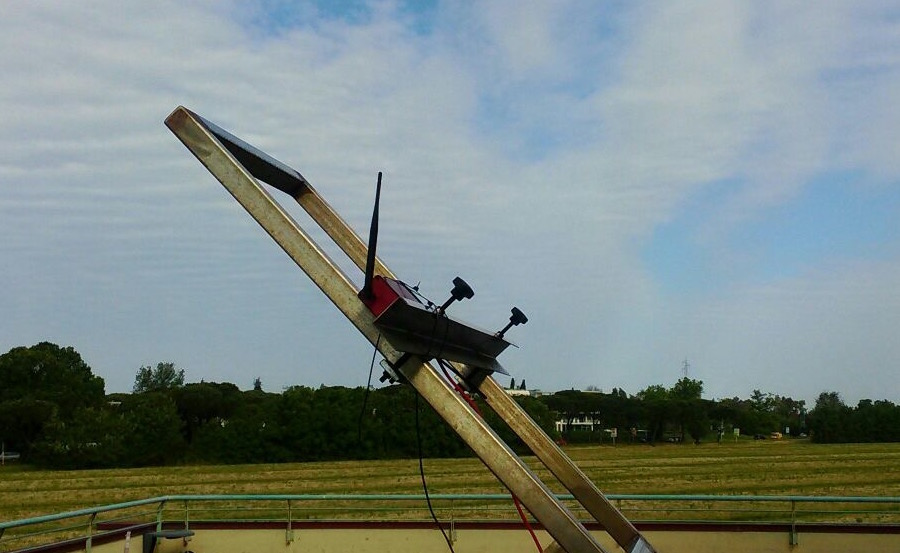
\includegraphics[width=.8\linewidth]{img/gateway}
\end{subfigure}%
\begin{subfigure}{.5\textwidth}
  \centering
  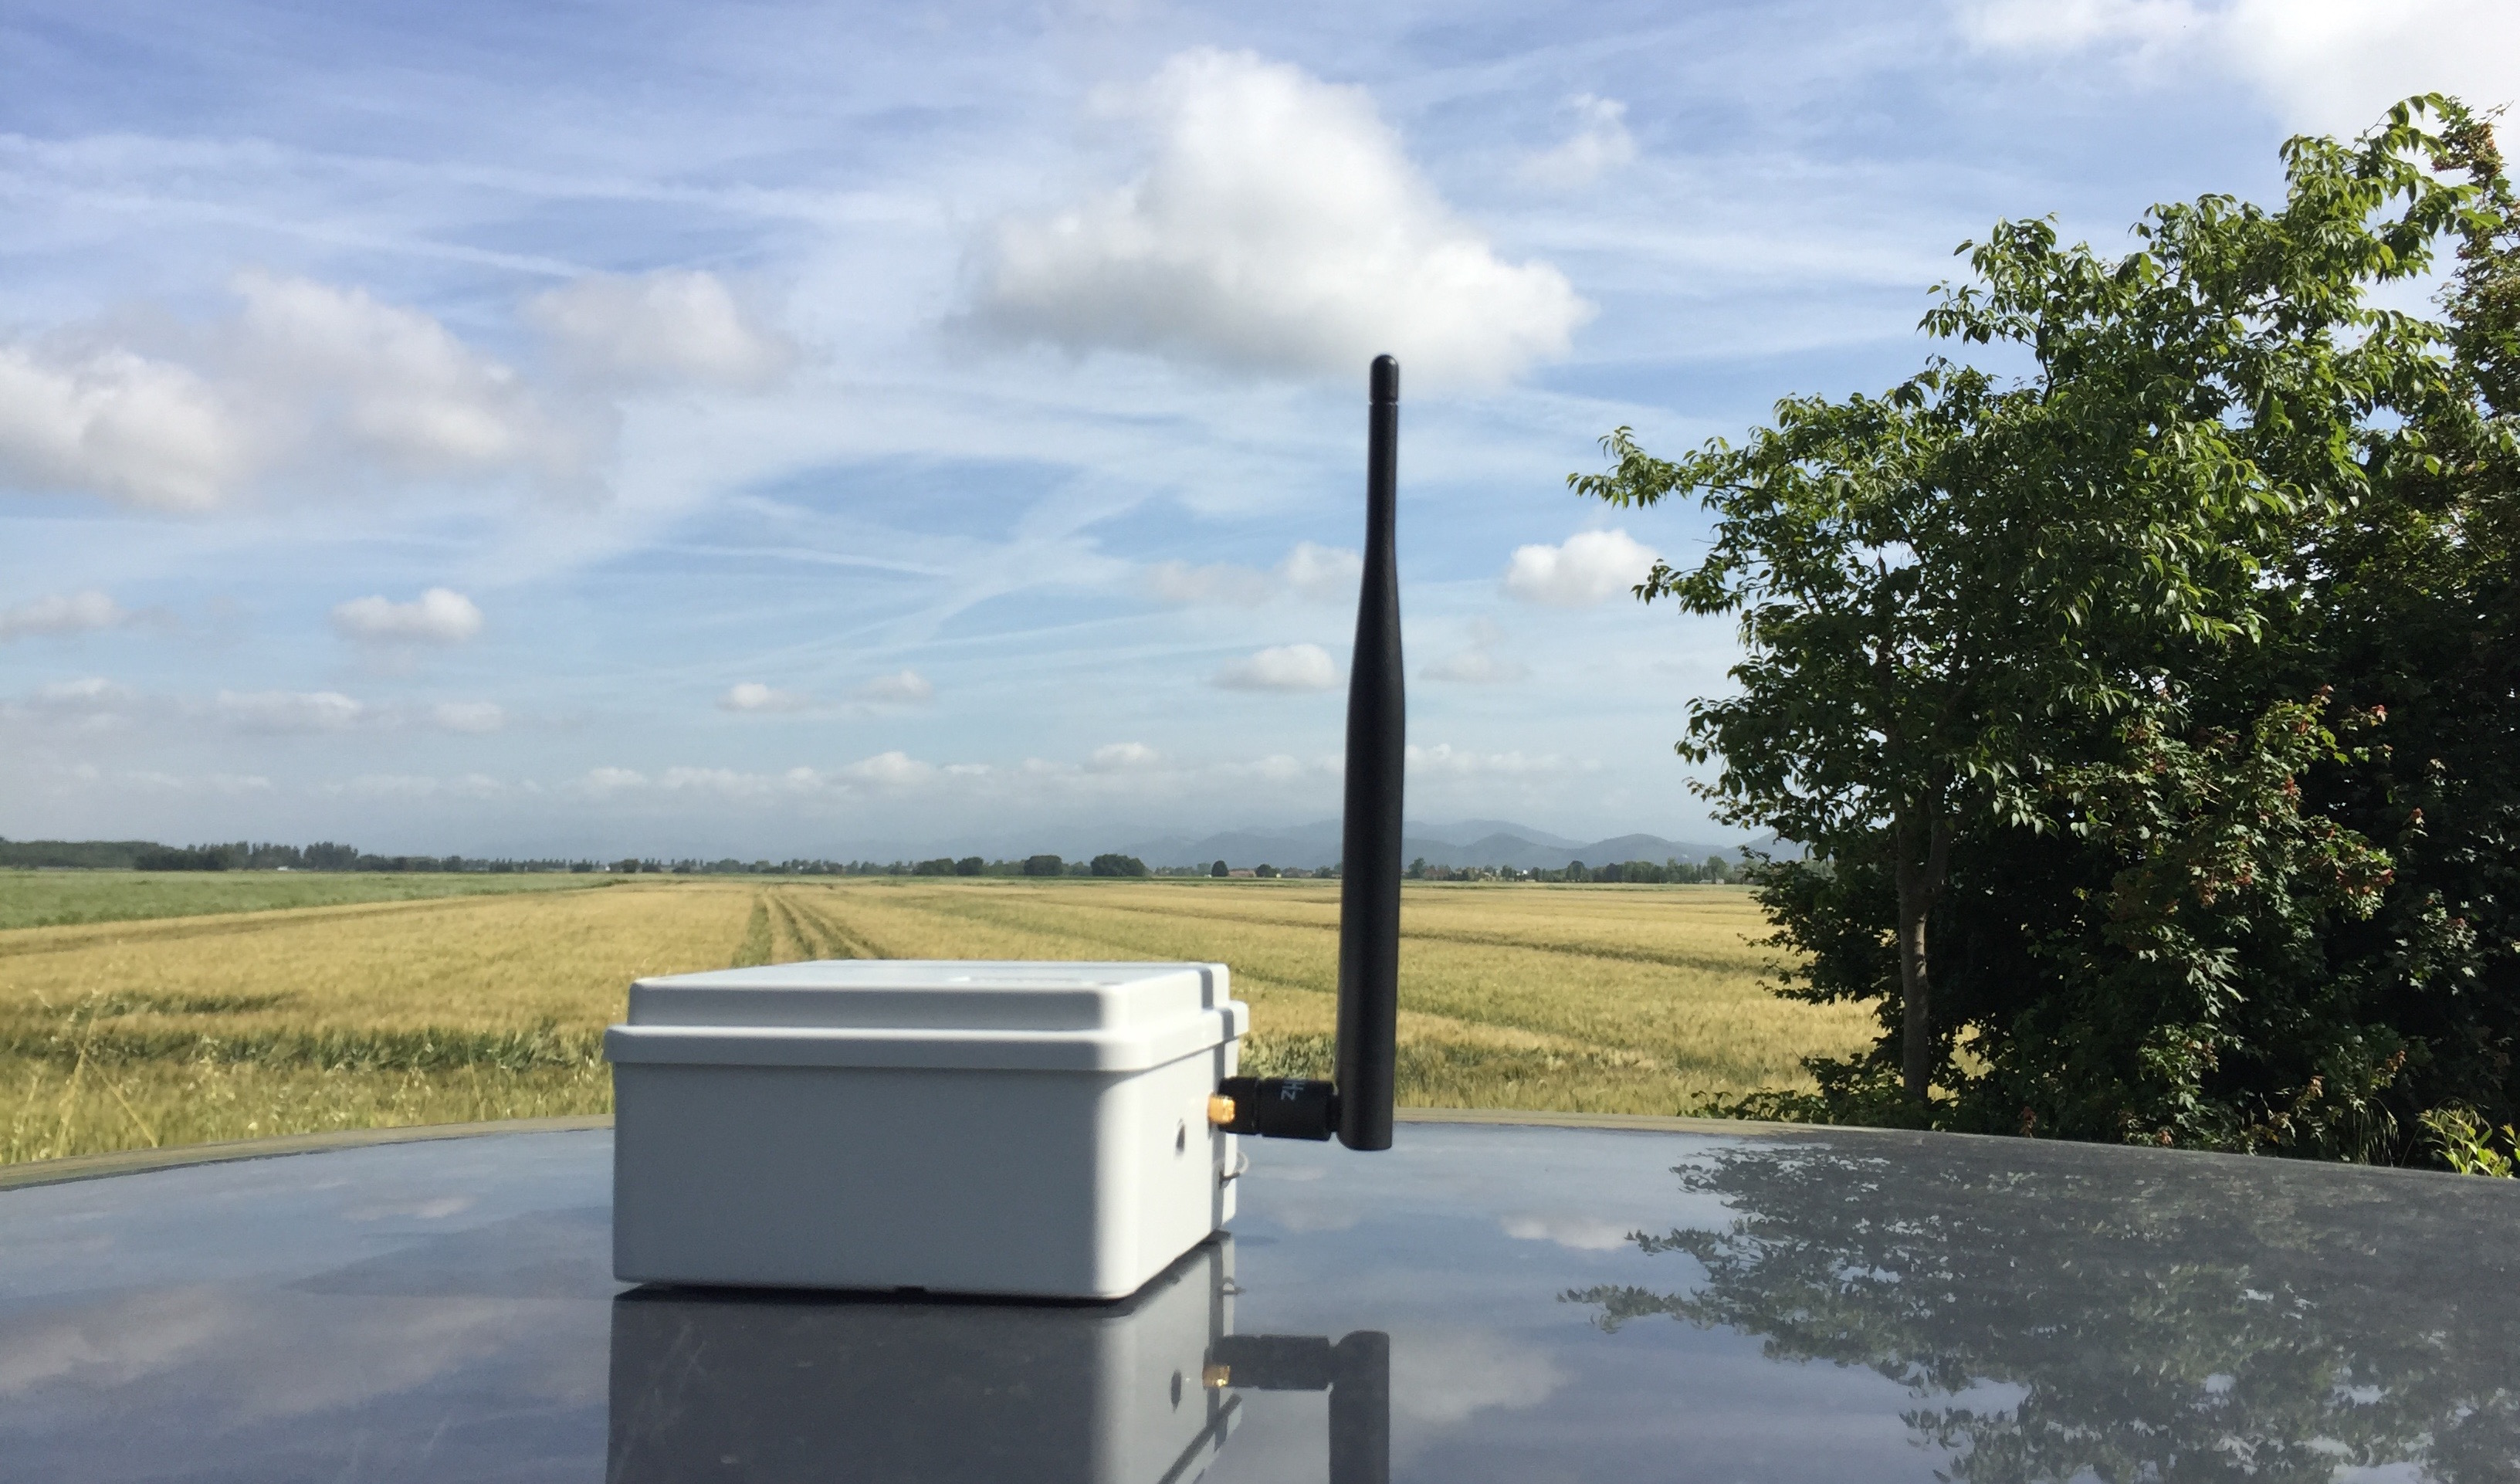
\includegraphics[width=.8\linewidth]{img/mote}
\end{subfigure}
\caption{The Lorank gateway and the Waspmote end-device}
\label{fig:test}
\end{figure}

The first set of experiments was performed in a rural environment with non line of sight condition. The gateway was placed on the terrace of the department of information engineering at the University of Pisa, located in Via Caruso 16, Pisa, Italy.

The end-devices were placed in different spots along a road inside the natural park of San Rossore, Pisa (Italy).

\begin{figure}[]
\centering
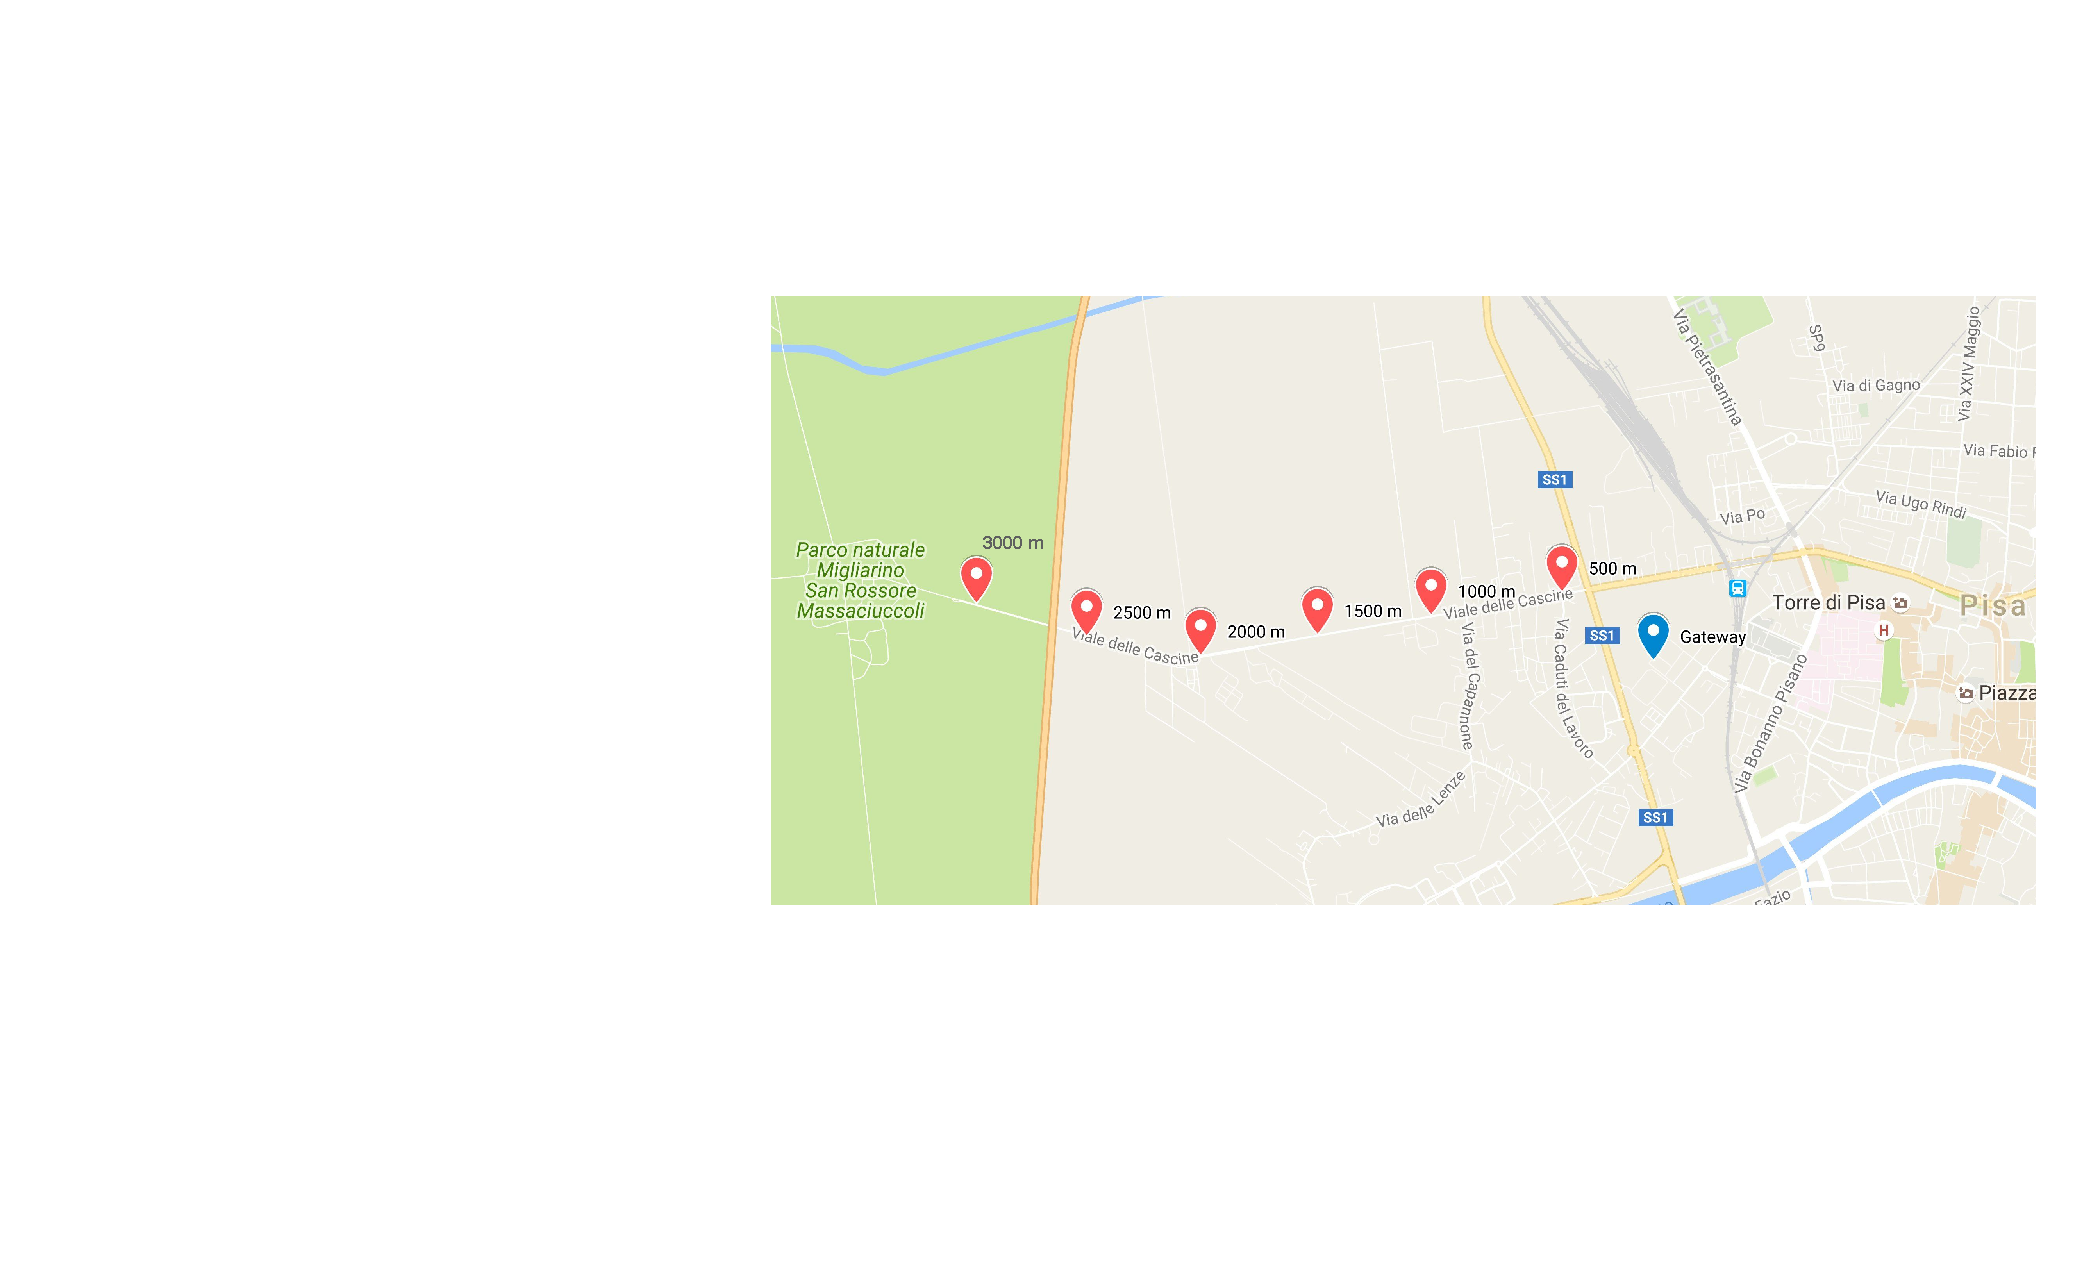
\includegraphics[width=\textwidth]{img/map_rural}
\caption{Map of rural experiments}
\label{fig:maprural}
\end{figure}


\subsection{Selection of parameters} 
Given these particular environments the parameters were chosen as follows:
\begin{itemize}
\item \emph{Data Rate}: all data rates were tested (from SF7BW125 to SF12BW125);
\item \emph{Coding Rate}: since in some preliminary tests it was discovered that the influence of the coding rate on the packet error rate in this environment was negligible, it was decided to test only 4/5;
\item \emph{Distance}: each end-device was placed starting from 500 meters away from the gateway up to 2500 meters, in steps of 500 meters;
\item \emph{Payload length}: 10 bytes and 50 bytes, to cover different real use cases;
\item \emph{Transmission power}: It was decided to test both the highest transmission power available and the lowest for which it is known from preliminary experiments to be strong enough to receive data.

So at 14 dBm and 8 dBm were tested at 1500, 2000 and 2500 meters. At 1000 meters 14 dBm and 5 dBm were tested, and at 500 meters away from the gateway 8 dBM and 2 dBm were tested.
\end{itemize}
Table \ref{tab:ruraltest} summarizes the chosen parameters.


% Please add the following required packages to your document preamble:
% \usepackage{booktabs}
\begin{table}[]
\centering
\caption{Rural test configurations}
\label{tab:ruraltest}
\begin{tabular}{@{}lll@{}}
\toprule
Parameter           & Values & Unit  \\ \midrule
Spreading factor    & 7, 8, 9, 10, 11, 12  &       \\
Coding Rate    & 4/5  &       \\
Transmission power  & 14, 8, 5 (1 Km), 2 (0.5 Km)  & dBm   \\
Payload length      & 10, 50 & bytes \\
Distance from gateway & 0.5, 1.0, 1.5, 2.0, 2.5 & Km    \\ \bottomrule
\end{tabular}
\end{table}

\subsection{Results}
Analyzing the results of this first set of experiments some peculiar behaviors has been discovered, in particular:
\begin{itemize}
\item up to 1500 meters away from the gateway (figure \ref{fig:sf7rural}) it is possible to transmit with the fastest data rate, which is SF7BW125, without having significant losses;

\item the length of the payload affects significantly the packet error rate only at 2500 meters and only with the slowest data rates, i.e. SF11 and SF12 (figures \ref{fig:sf11rural} and \ref{fig:sf12rural}); 

\item At 500 meters, using data rate SF12, it was obtained an higher packet error rate than the faster, and less robust, data rates. In particular the performances of SF12 are significantly worse than SF11, with the same transmission power, and the results with 8 dBm were slightly worse than same data rate with 2 dBm. This strange results are caused by the electric field intensity and the received power over flat terrain.
\end{itemize}


\begin{figure}[]
\centering
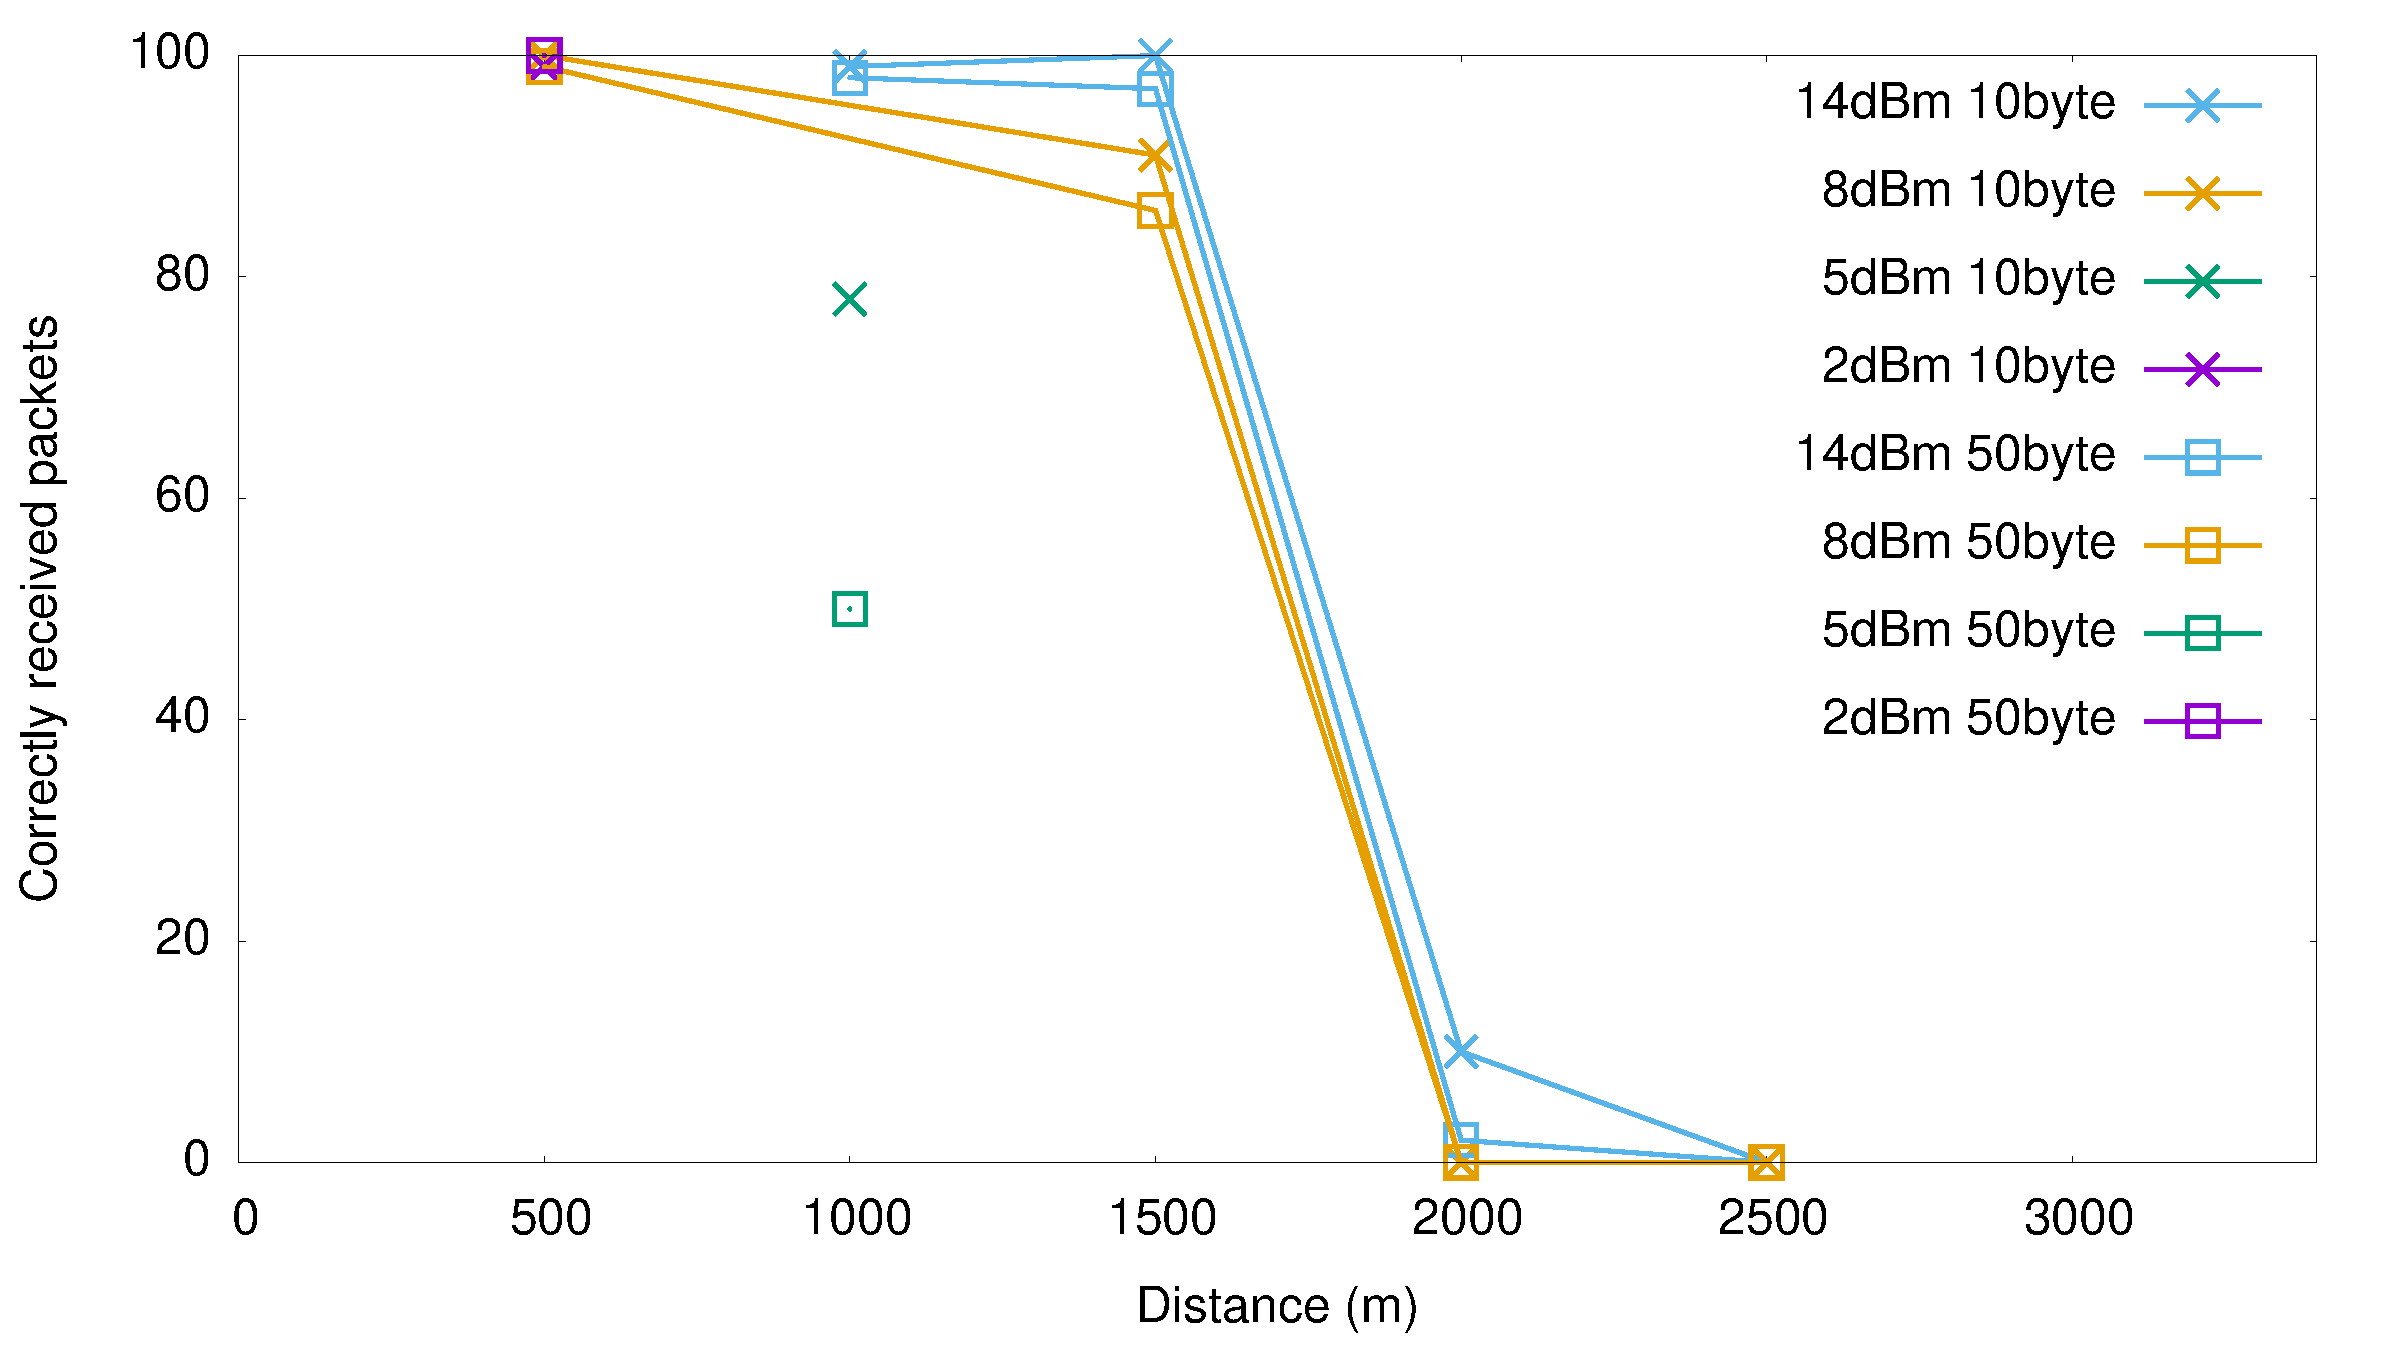
\includegraphics[width=\textwidth]{img/test/rural/sf7}
\caption{Results of rural experiments at SF 7}
\label{fig:sf7rural}
\end{figure}

\begin{figure}[]
\centering
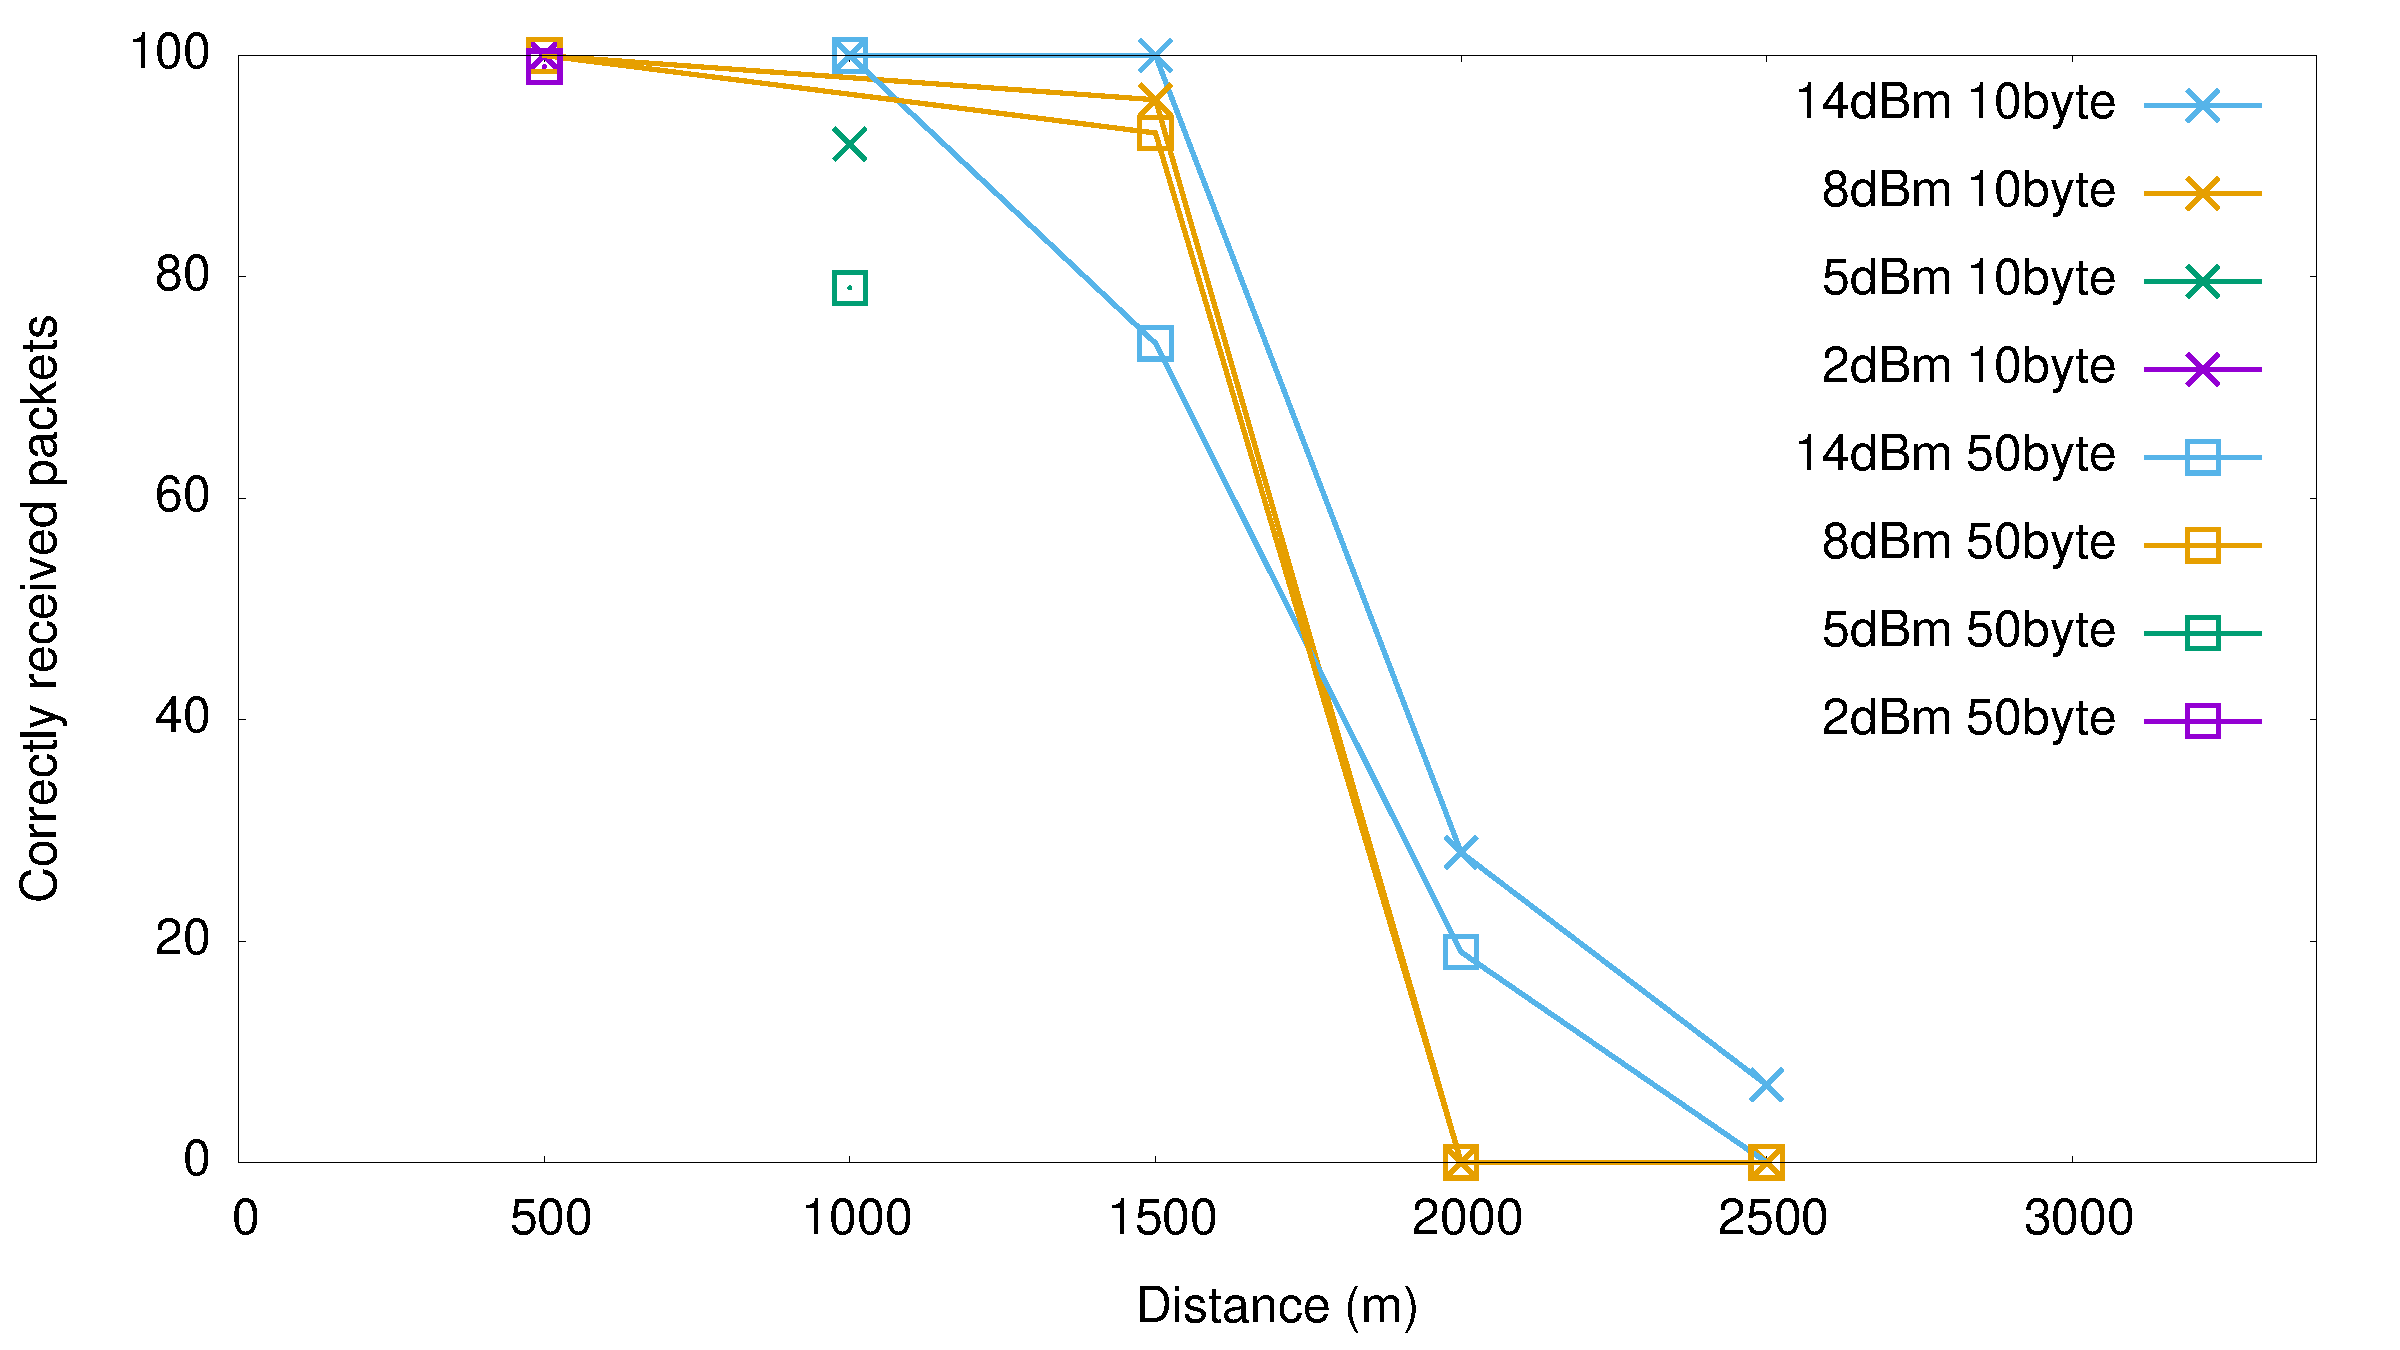
\includegraphics[width=\textwidth]{img/test/rural/sf8}
\caption{Results of rural experiments at SF 8}
\label{fig:sf8rural}
\end{figure}

\begin{figure}[]
\centering
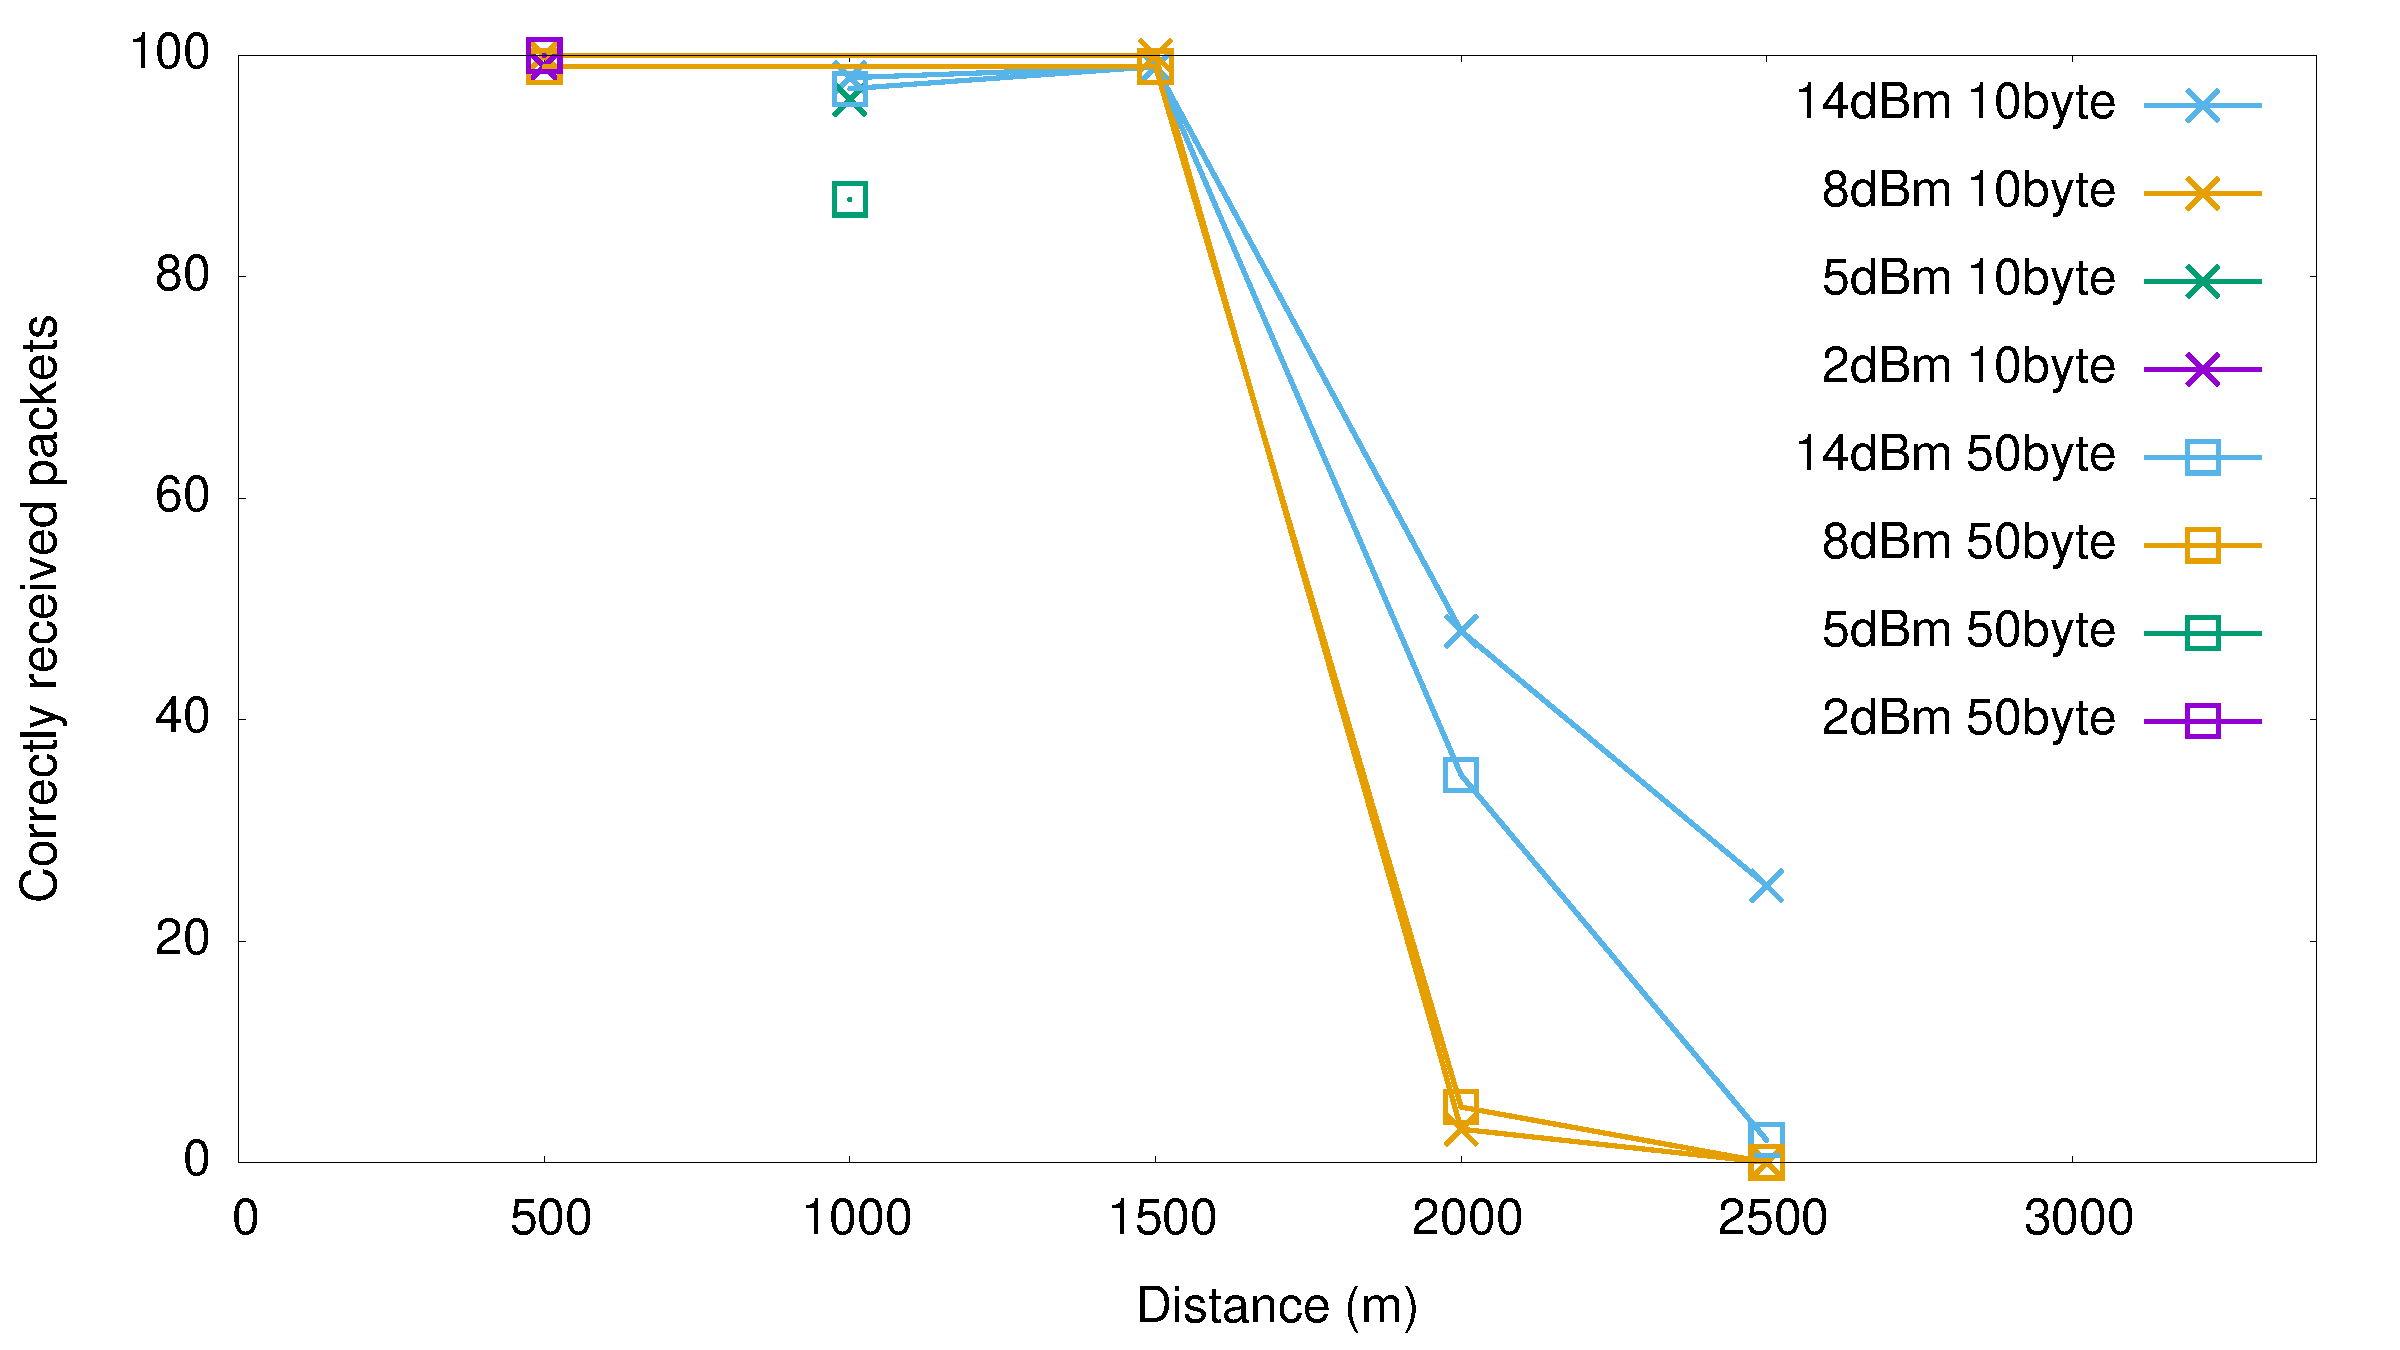
\includegraphics[width=\textwidth]{img/test/rural/sf9}
\caption{Results of rural experiments at SF 9}
\label{fig:sf9rural}
\end{figure}

\begin{figure}[]
\centering
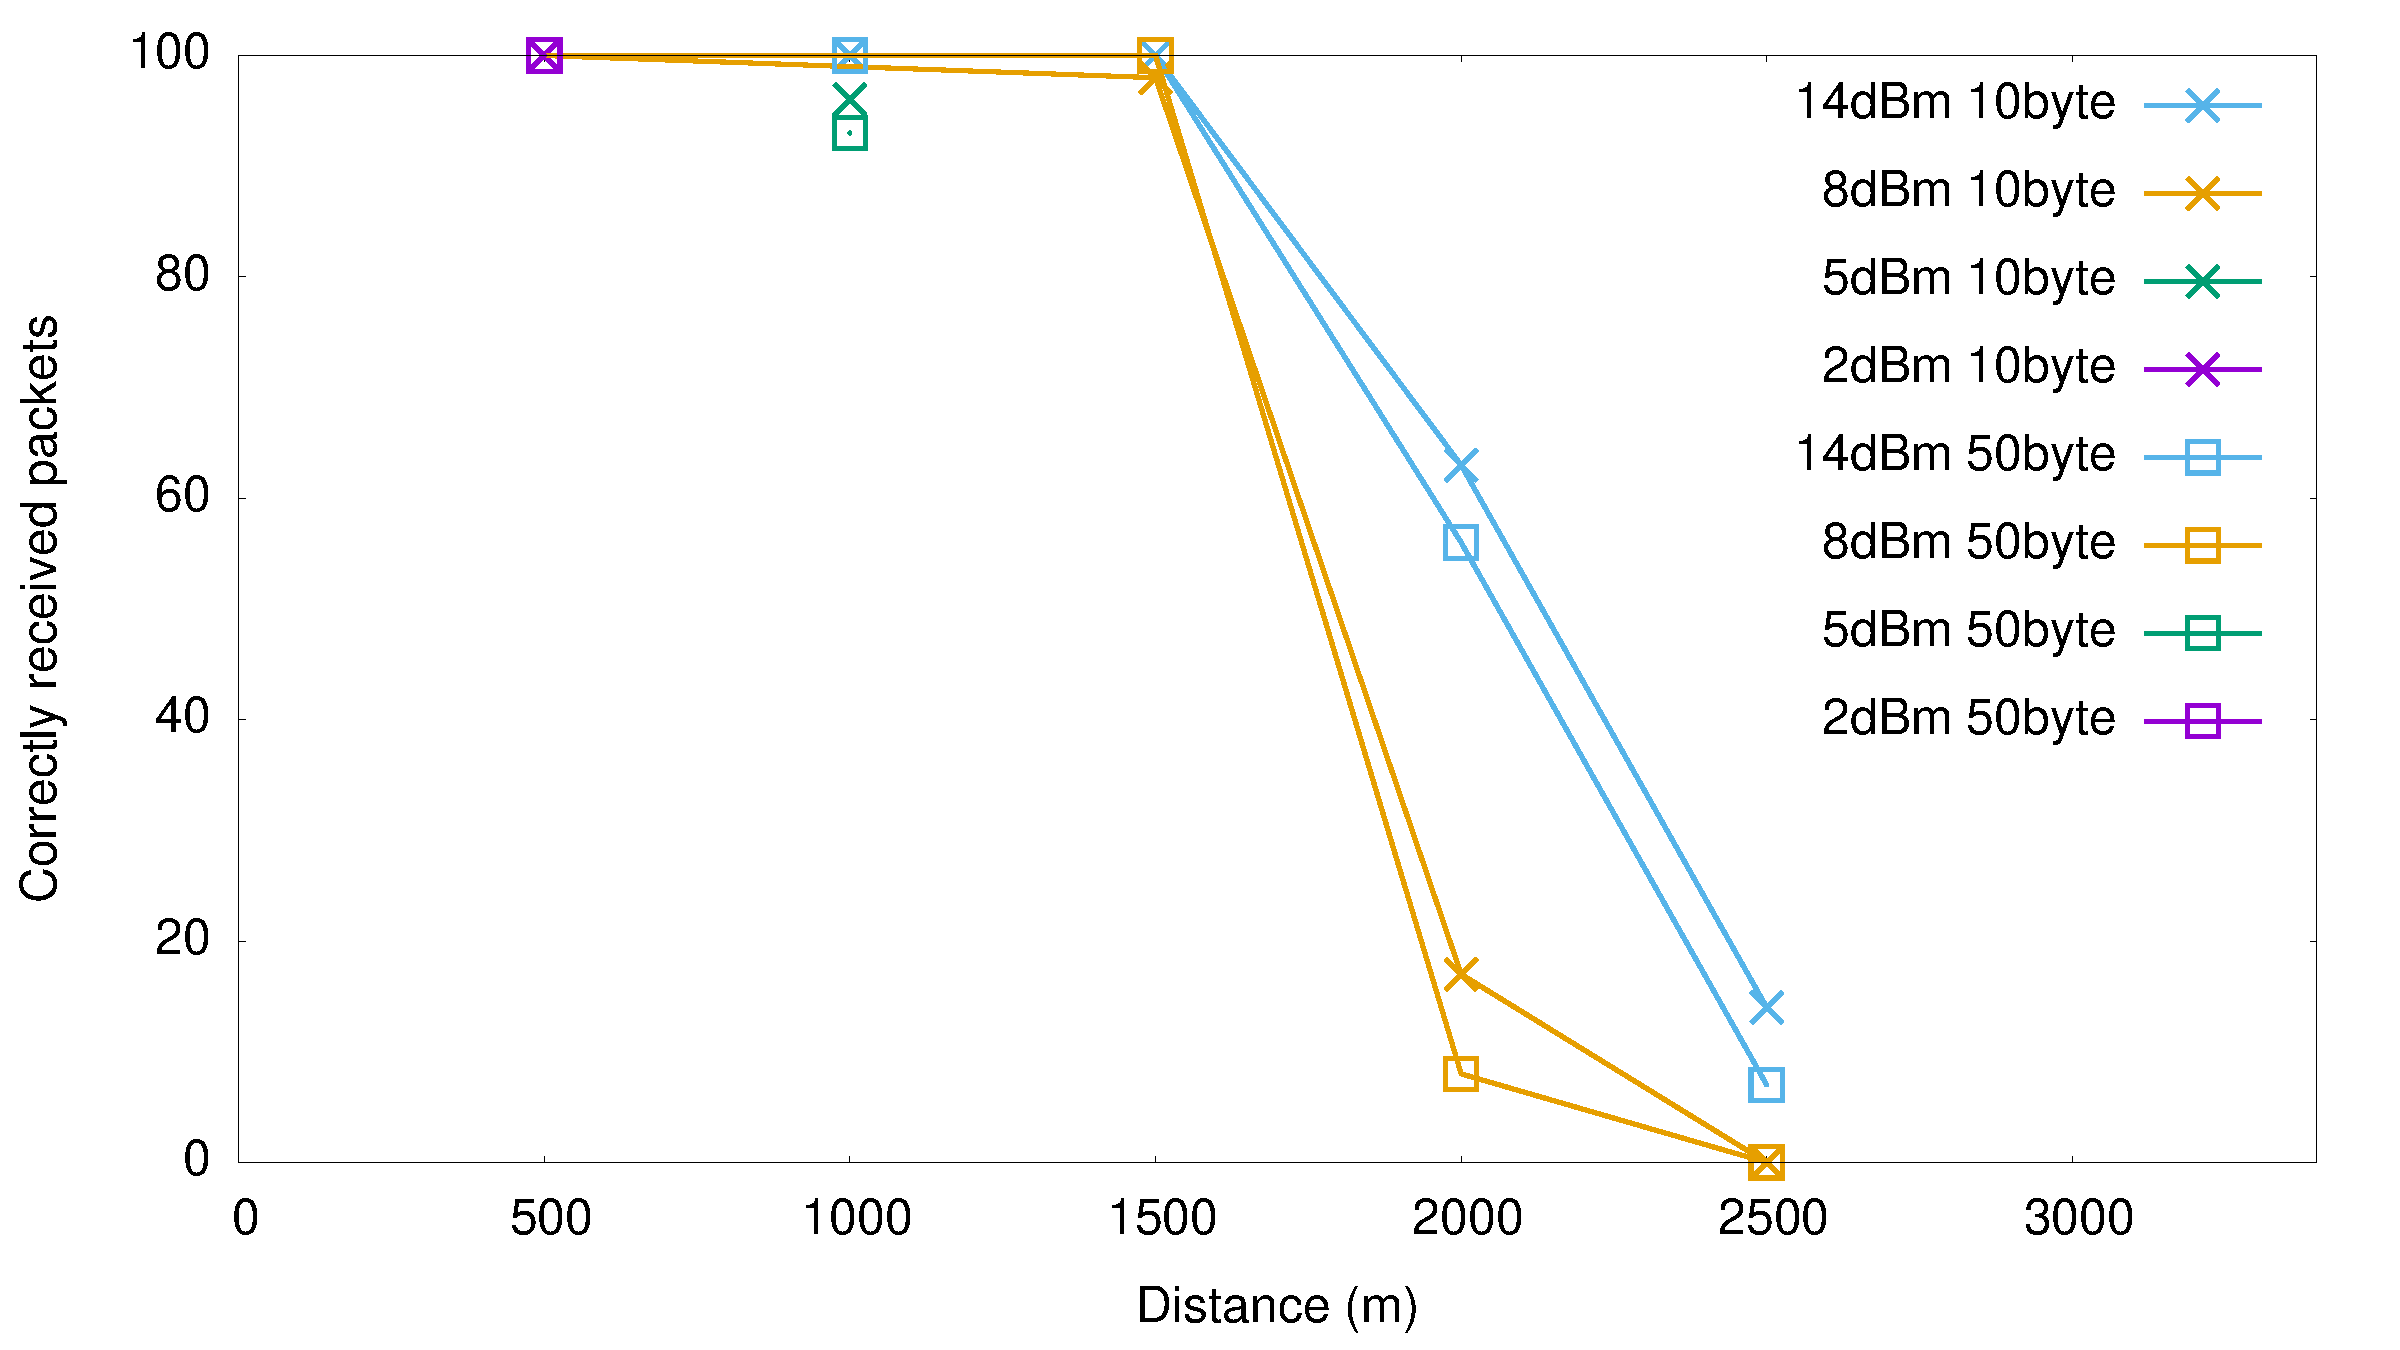
\includegraphics[width=\textwidth]{img/test/rural/sf10}
\caption{Results of rural experiments at SF 10}
\label{fig:sf10rural}
\end{figure}

\begin{figure}[]
\centering
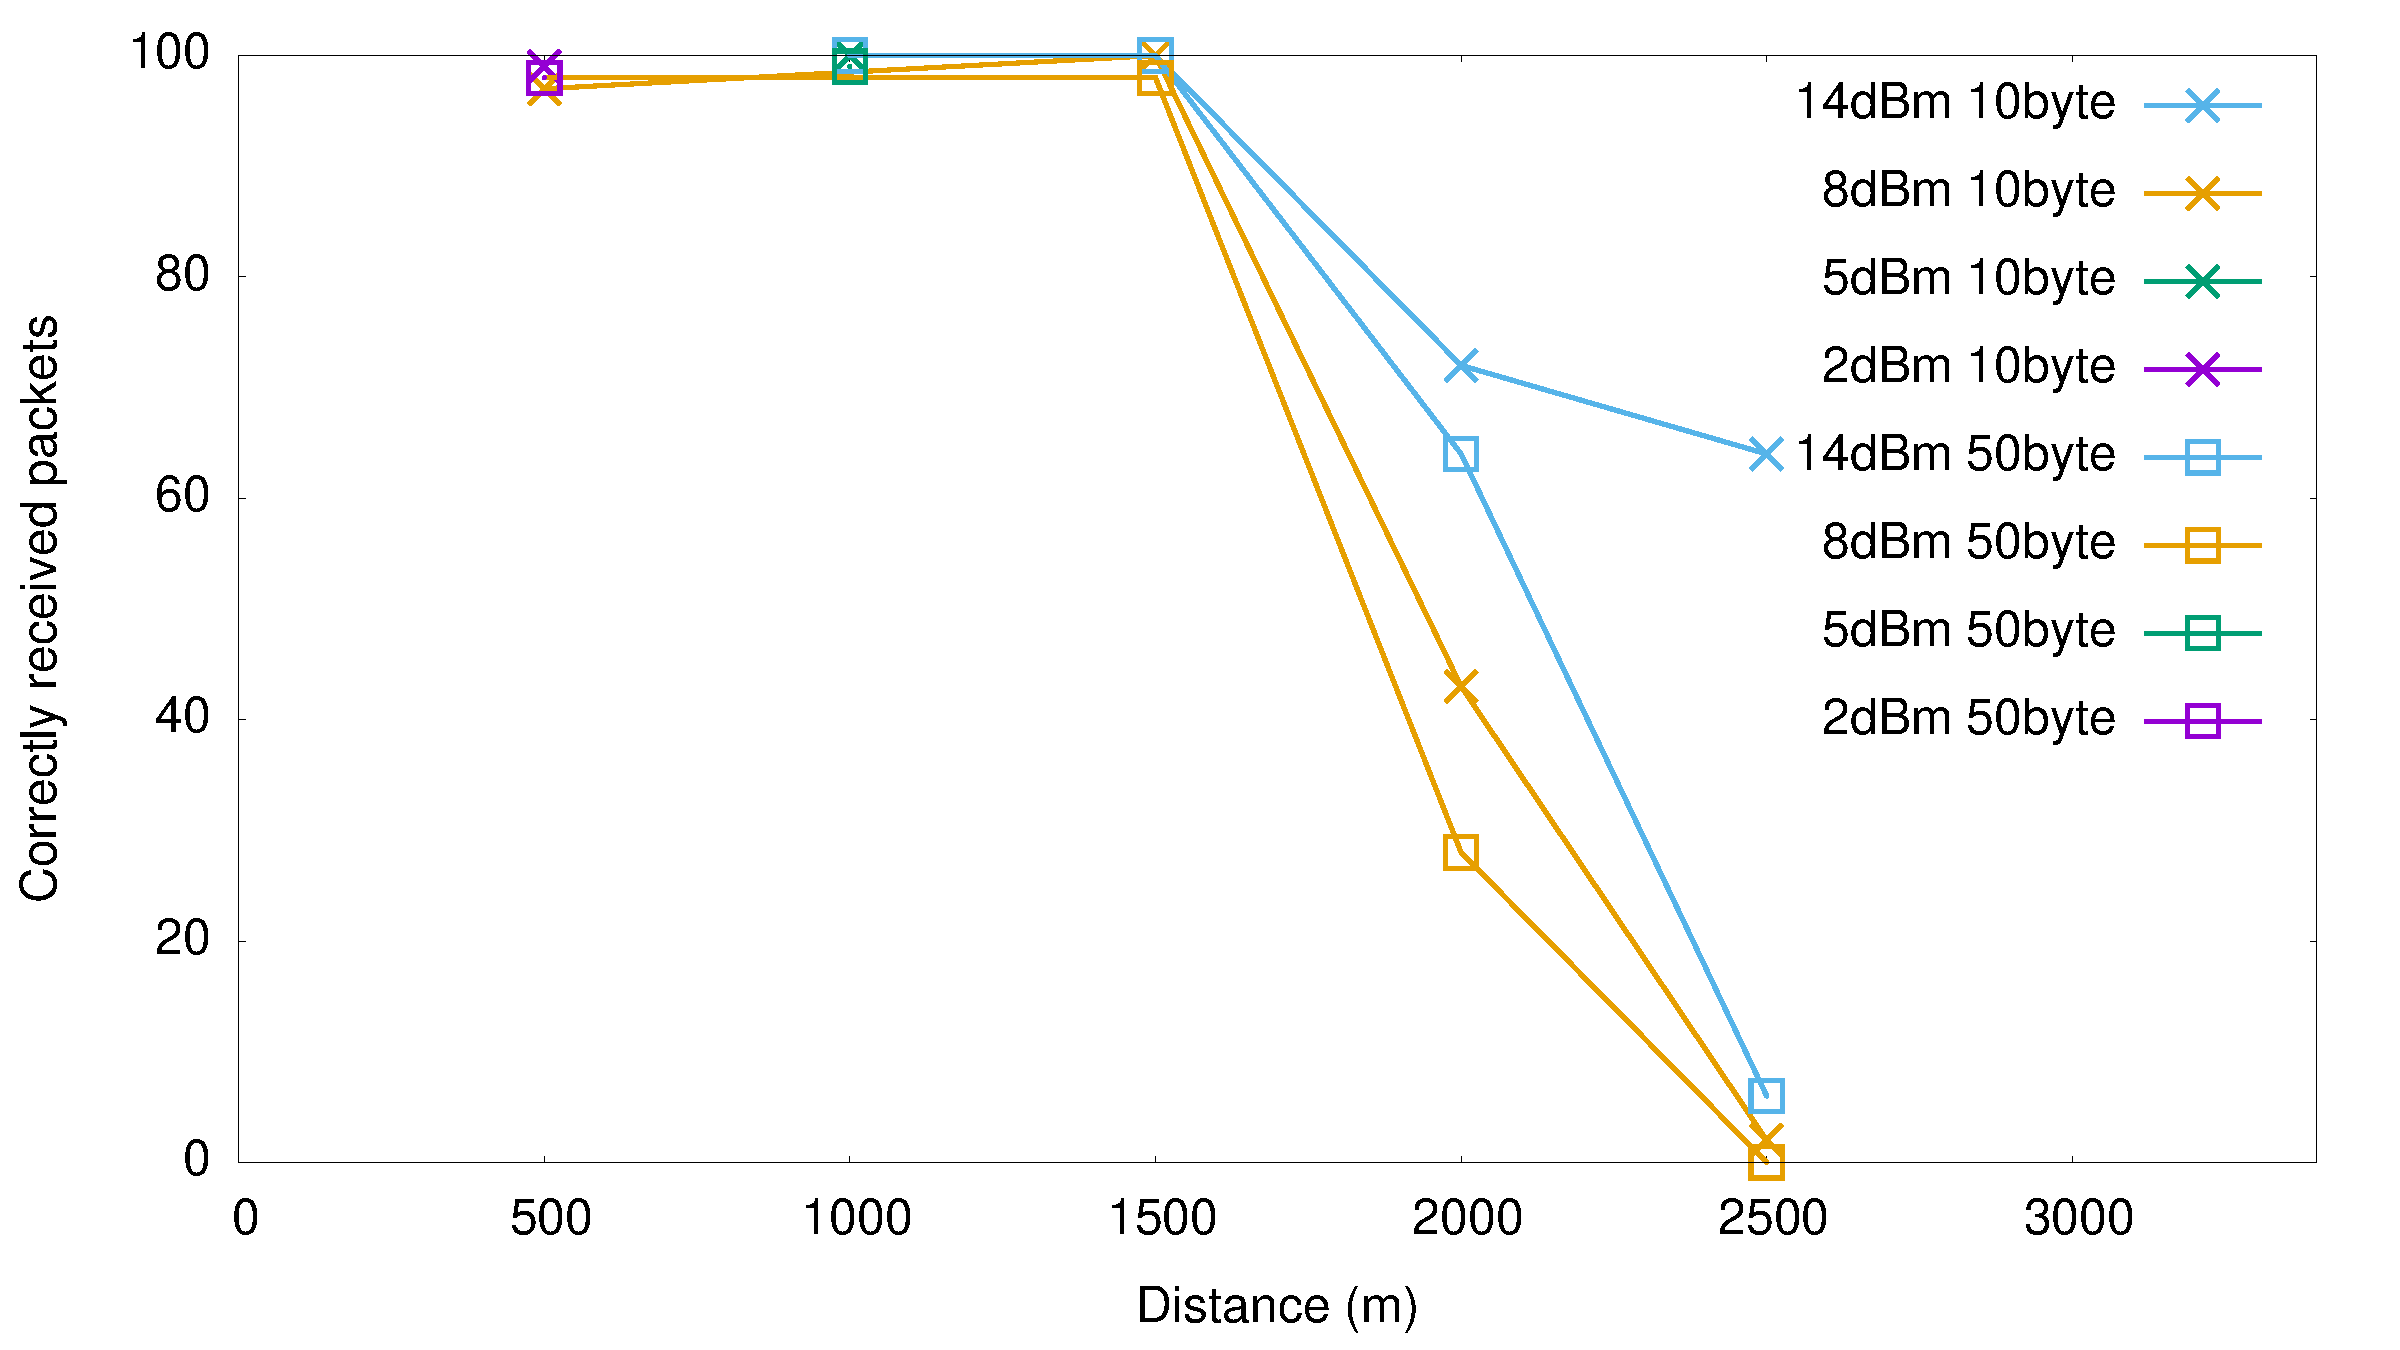
\includegraphics[width=\textwidth]{img/test/rural/sf11}
\caption{Results of rural experiments at SF 11}
\label{fig:sf11rural}
\end{figure}

\begin{figure}[]
\centering
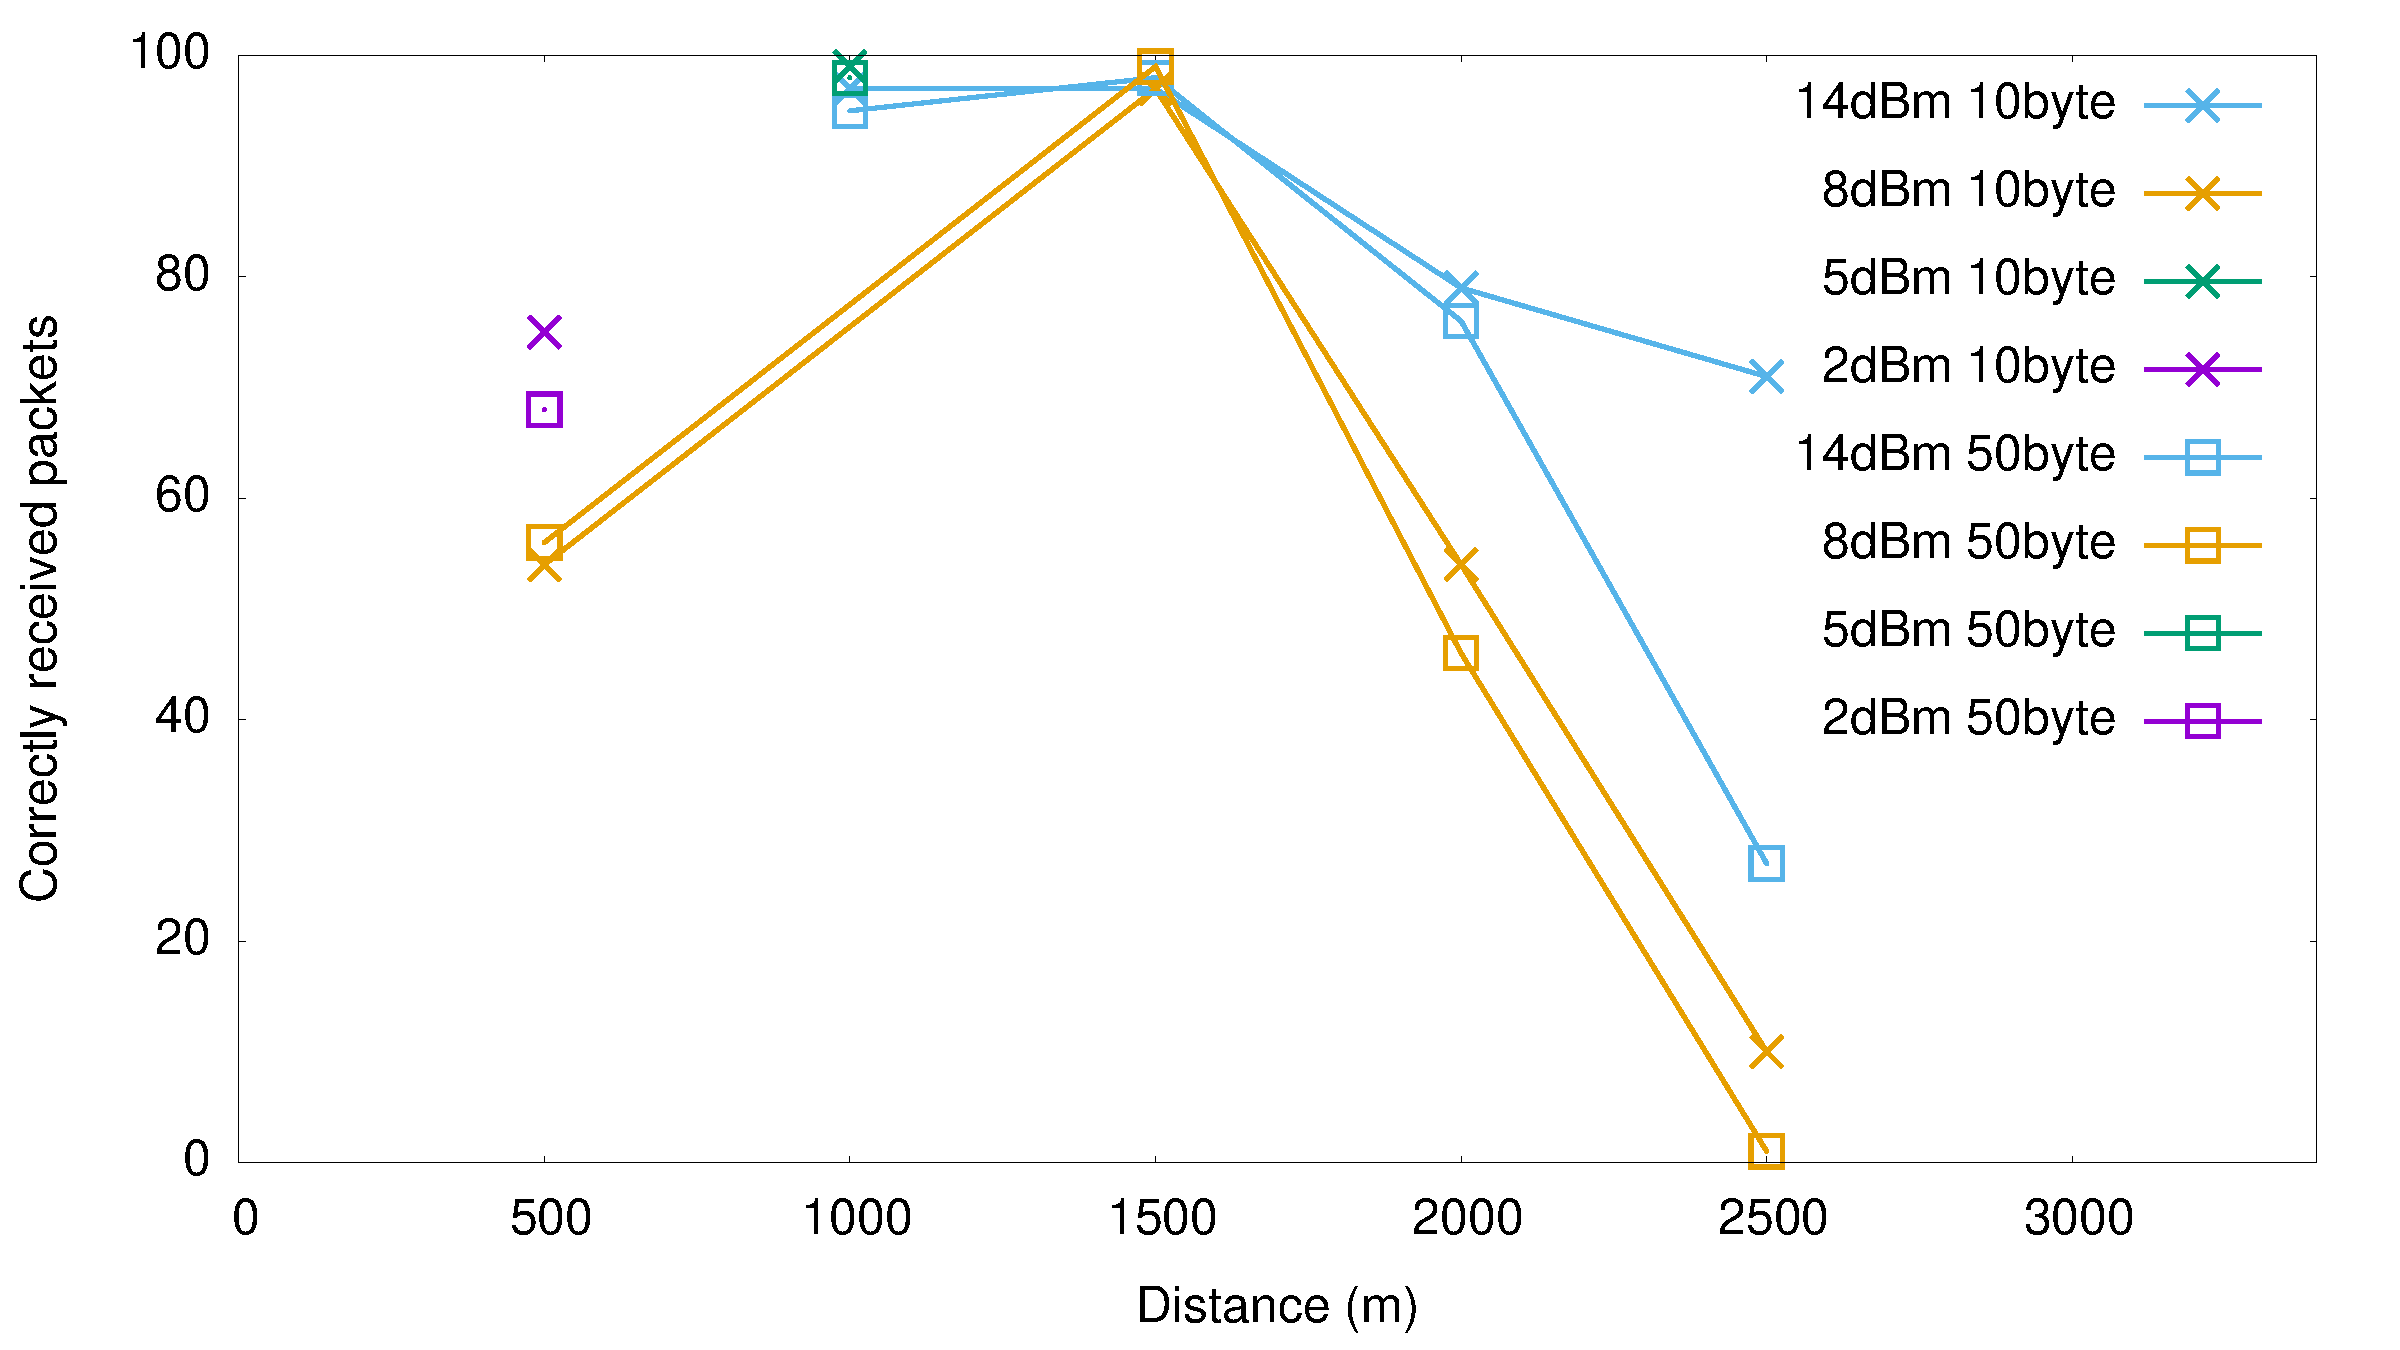
\includegraphics[width=\textwidth]{img/test/rural/sf12}
\caption{Results of rural experiments at SF 12}
\label{fig:sf12rural}
\end{figure}


\newpage
\section{Urban experiments}

The urban experiments were performed in the city center of Pisa. The gateway was placed in front of a window at the fifth floor of department of information engineering, section computer engineering, at the University of Pisa, located in Largo Lucio Lazzarino 1, Pisa, Italy.

The end-device was placed inside, at the first floor of a building located in Via Risorgimento, Pisa. The area between the two devices is a typical urban area with three-floor buildings in the middle.

\begin{figure}[]
\centering
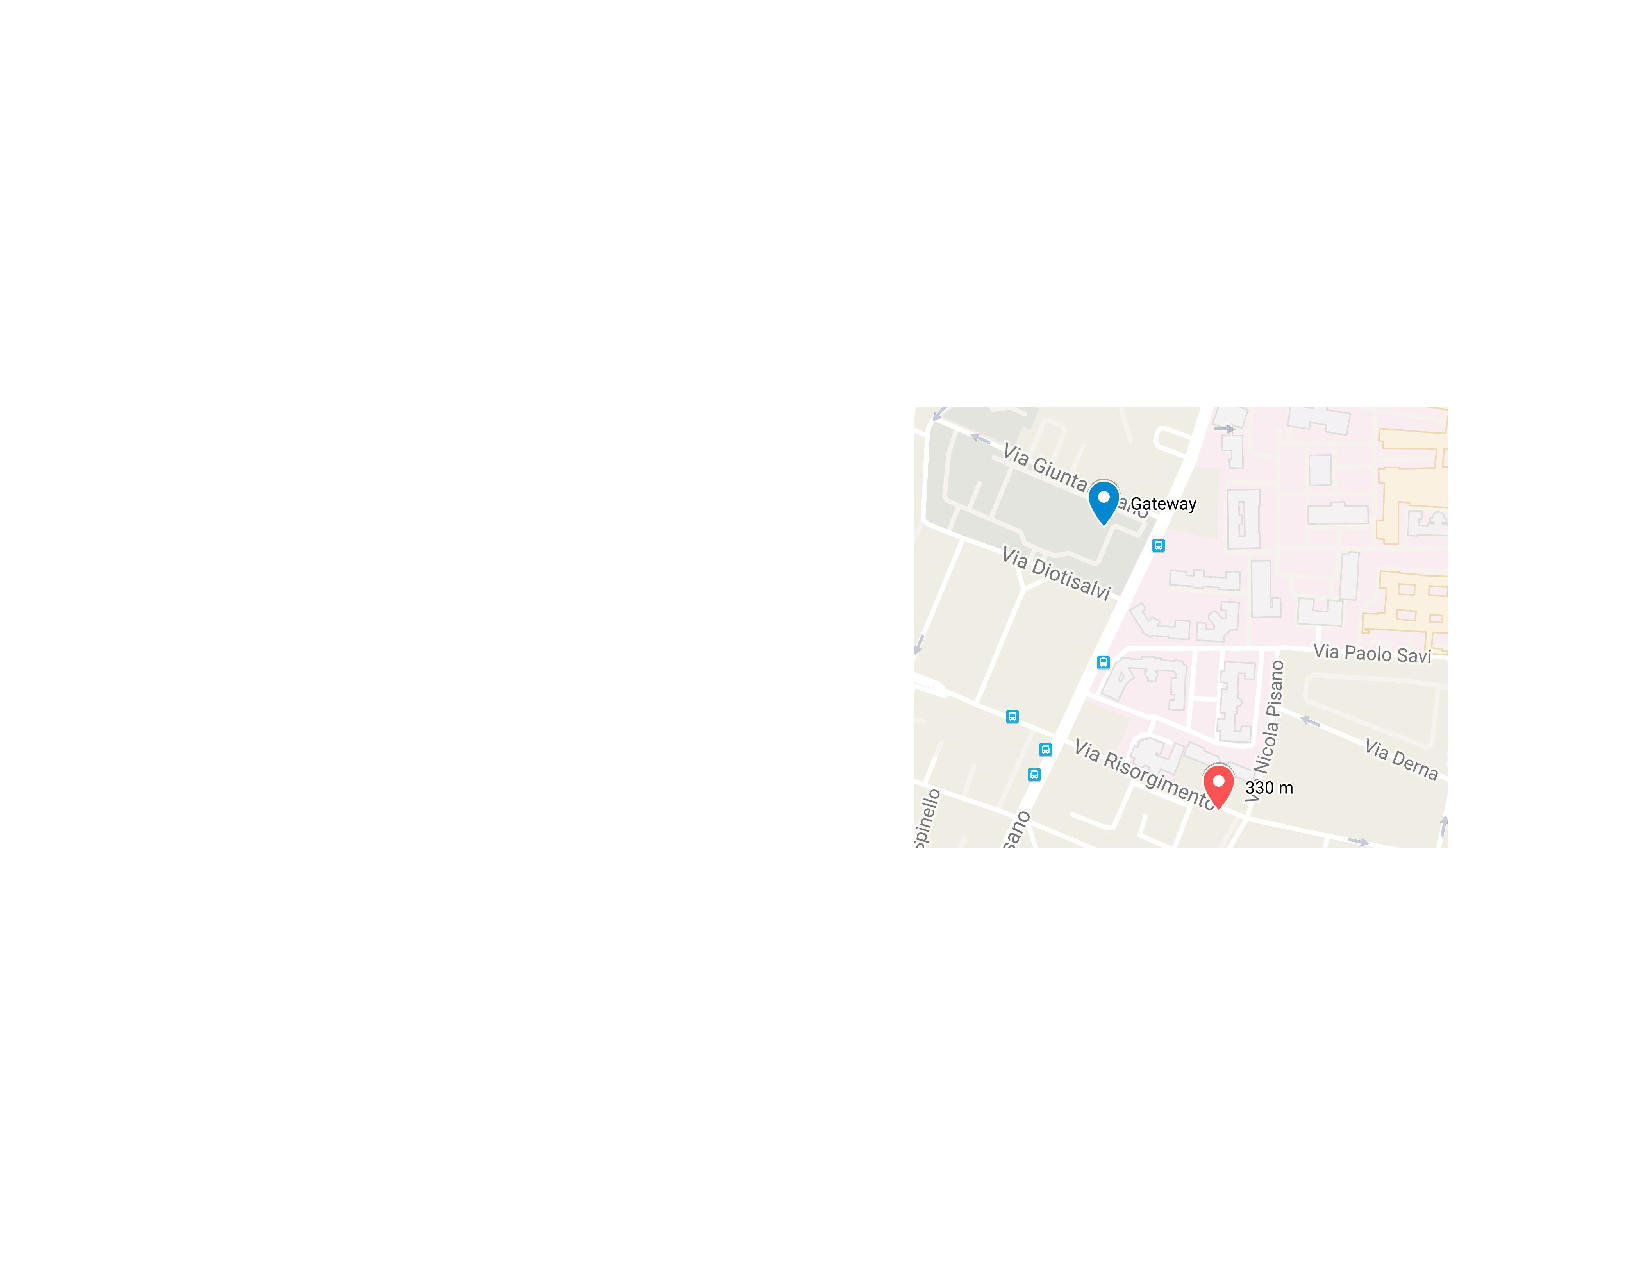
\includegraphics[width=.7\textwidth]{img/map_urban}
\caption{Map of urban experiments}
\label{fig:mapurban}
\end{figure}


\subsection{Selection of parameters} 

For this set of experiments, rather than distances with fixed steps, it was decided to choose some fixed location and try to test all possibles configurations. Since the range of coverage is substantially smaller than in rural test, it was decided also to evaluate the impact of an higher forward error correction, determined by the coding rate, on the reliability of the link.

The parameters were chosen as follows:
\begin{itemize}
\item \emph{Data Rate}: all data rates were tested (from SF7BW125 to SF12BW125);
\item \emph{Coding Rate}: the lowest level of FEC, 4/5, and the highest one, 4/8, were tested;
\item \emph{Distance}: each end-device was placed in a fixed location inside a building; in this section are presented only the results obtained at 330 meters away from the gateway;
\item \emph{Payload length}: 10 bytes and 50 bytes, to cover different real use cases;
\item \emph{Transmission power}: 14, 8, 5, 2 dBm in order to complete explore the impact of the reduction of transmission power on the packet error rate.
\end{itemize} 
Table \ref{tab:urbantest} summarizes the chosen parameters.

% Please add the following required packages to your document preamble:
% \usepackage{booktabs}
\begin{table}[]
\centering
\caption{Urban test configurations}
\label{tab:urbantest}
\begin{tabular}{@{}lll@{}}
\toprule
Parameter           & Values & Unit  \\ \midrule
Spreading factor    & 7, 8, 9, 10, 11, 12  &       \\
Coding Rate    & 4/5, 4/8  &       \\
Transmission power  & 14, 8, 5, 2  & dBm   \\
Payload length      & 10, 50 & bytes \\
Distance from gateway & 0.33 & Km    \\ \bottomrule
\end{tabular}
\end{table}


\subsection{Results}
From the results of this experiments it is possible to notice that, as expected, transmission with an higher level of \emph{forward error correction} are more reliable than the other ones, but in general the variation of the \emph{coding rate} does not substantially improve performance, especially with shorter packets;

However, in border cell condition the impact of the \emph{coding rate} is considerably high. It is possible to appreciate this behavior in particularly for spreading factor 9 (figure \ref{fig:sf9urban}): considering experiments with payload of 50 bytes, it is possible to notice that in extreme conditions, i.e. the best and worst transmission power, there is no difference of behavior between two different coding rates. Instead, for 5 and 8 dBm, the higher coding rate makes really the difference, making the channel a lot more reliable than with lower coding rate.

Regarding the other parameters, both \emph{payload length} and \emph{transmission power} behaved as expected from theory.

\begin{figure}[]
\centering
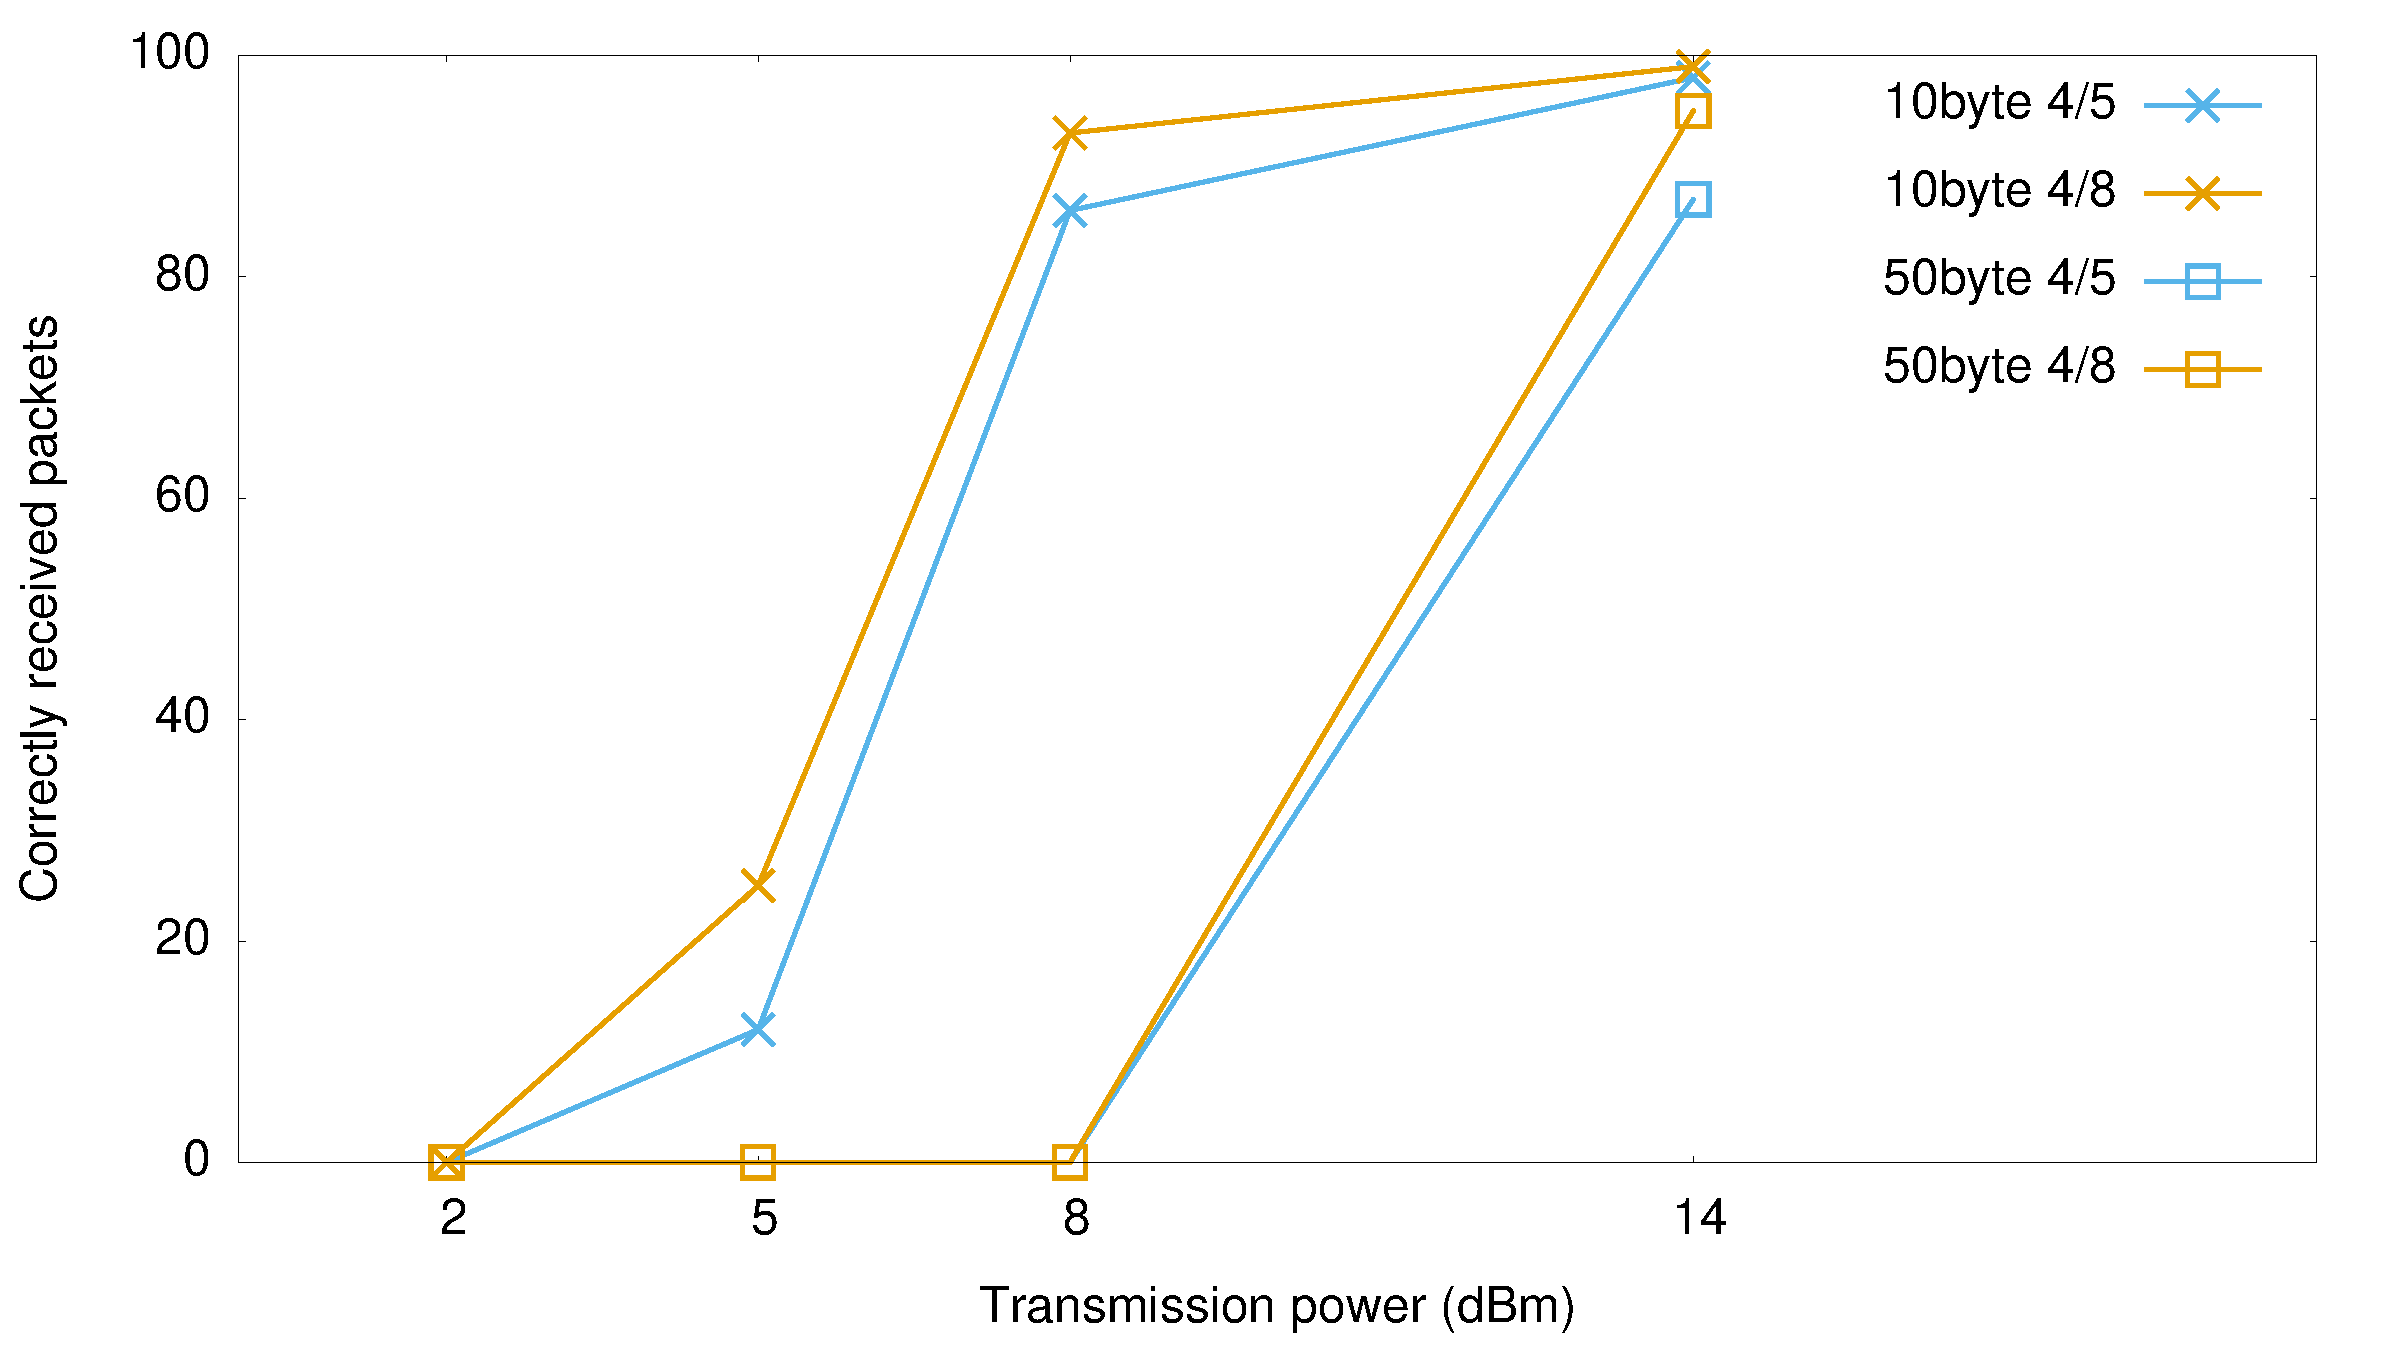
\includegraphics[width=\textwidth]{img/test/urban/sf7}
\caption{Results of urban experiments at SF 7}
\label{fig:sf7urban}
\end{figure}

\begin{figure}[]
\centering
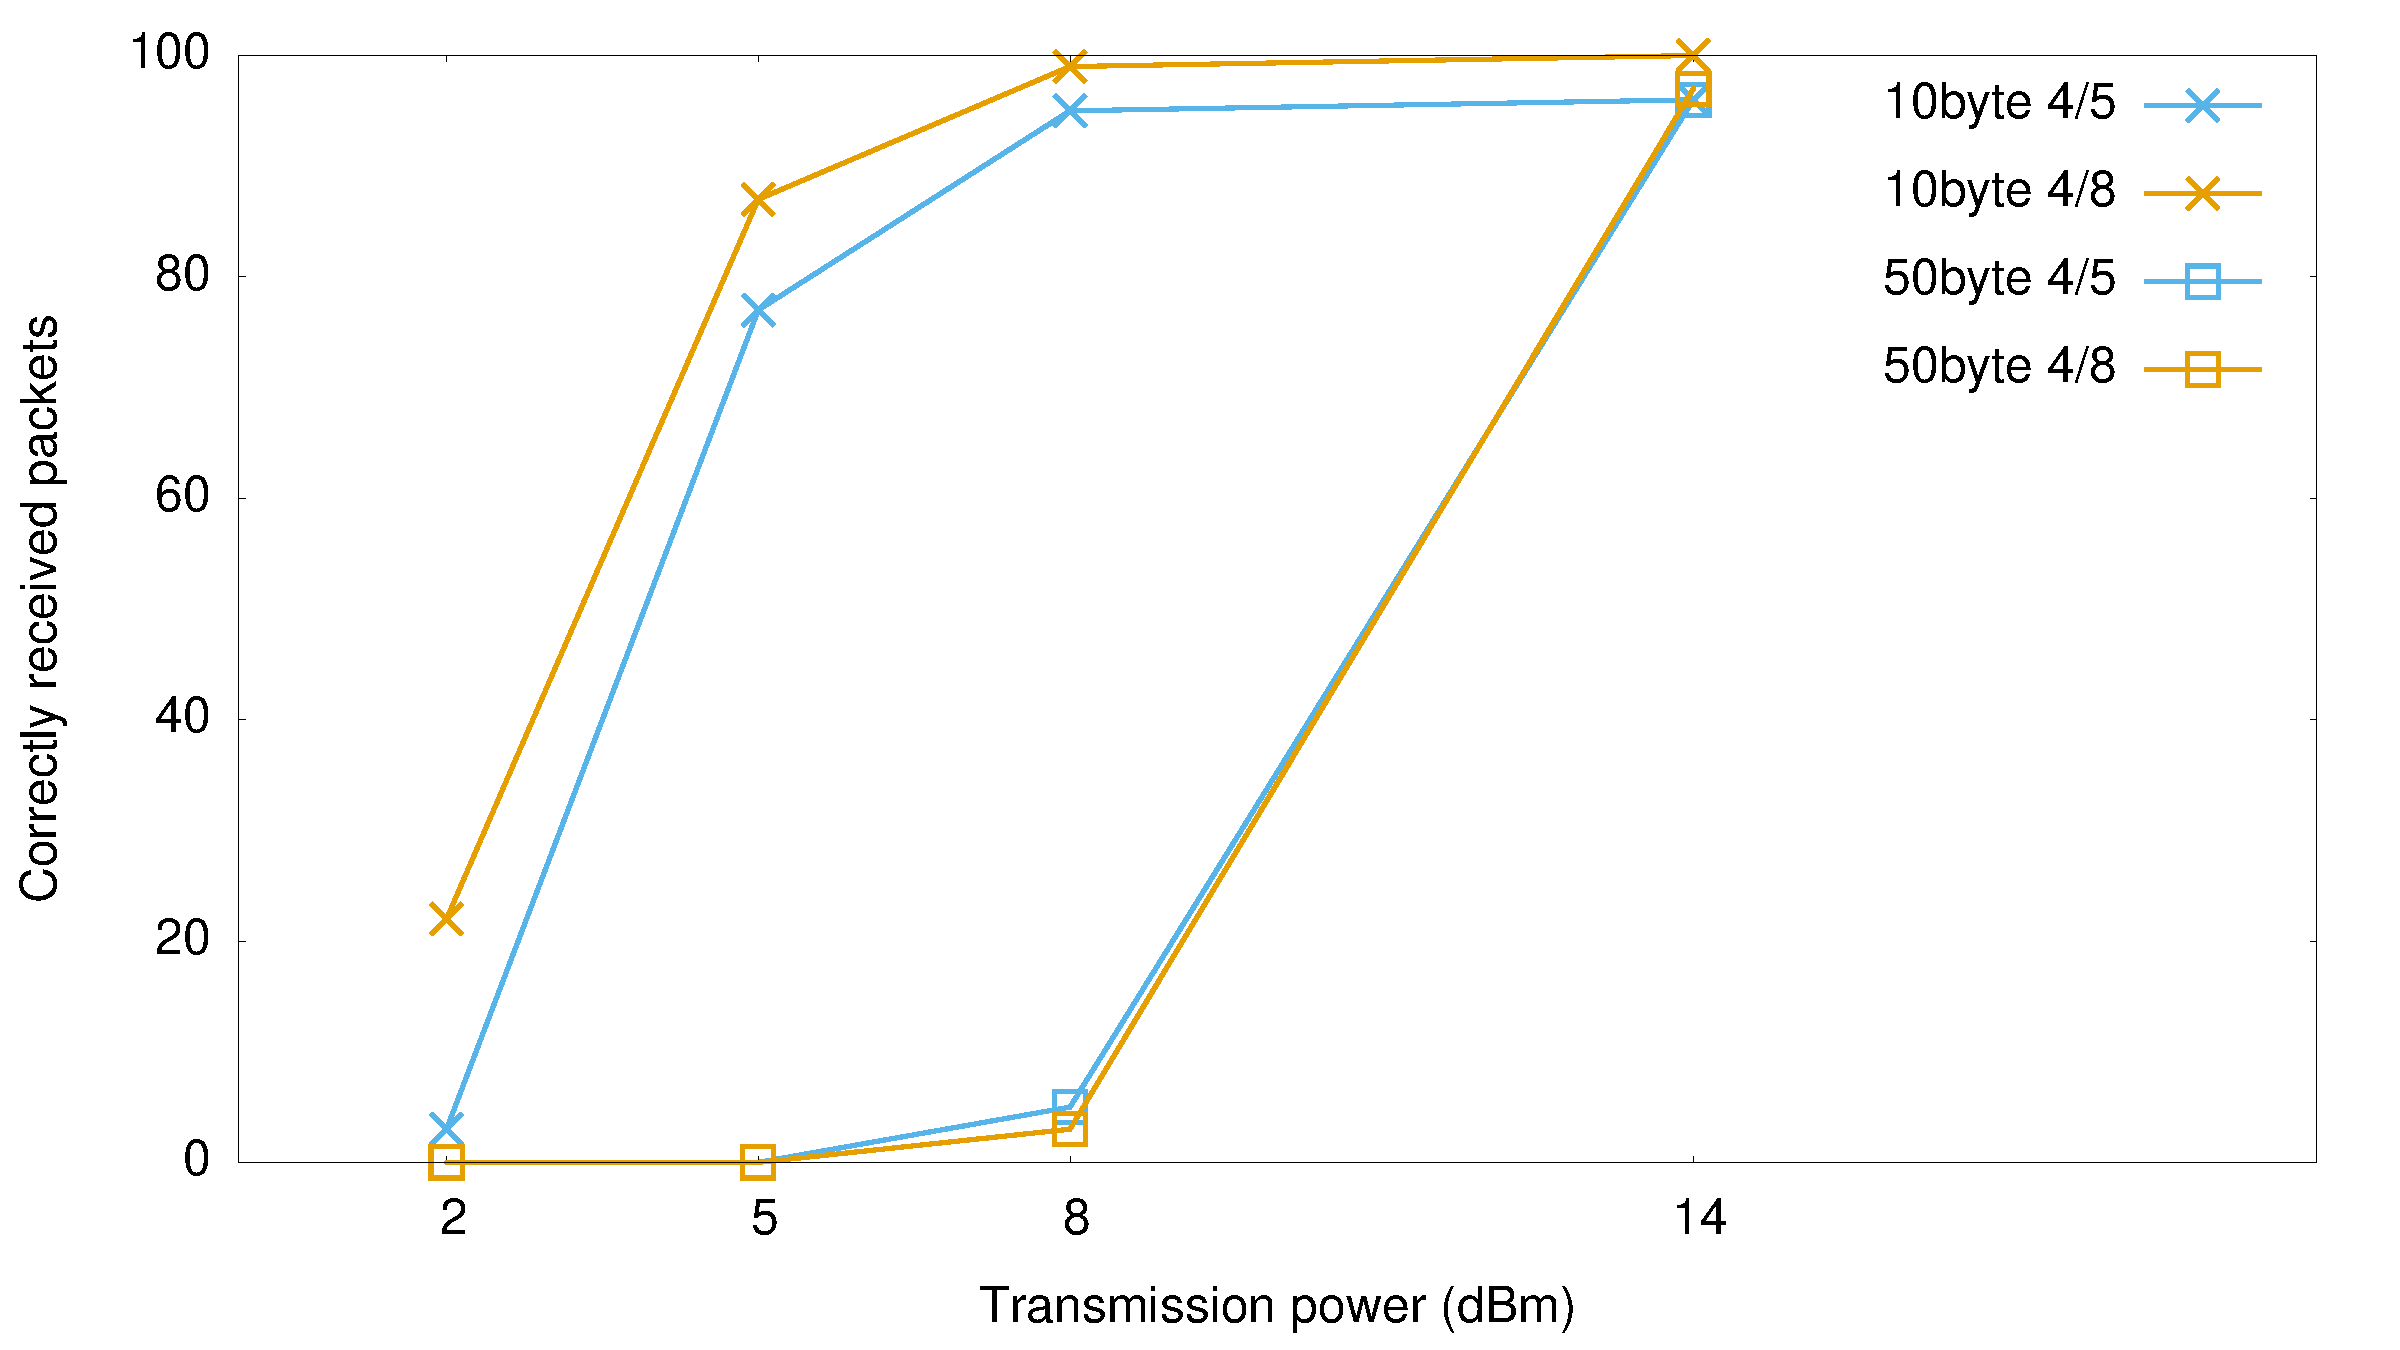
\includegraphics[width=\textwidth]{img/test/urban/sf8}
\caption{Results of urban experiments at SF 8}
\label{fig:sf8urban}
\end{figure}

\begin{figure}[]
\centering
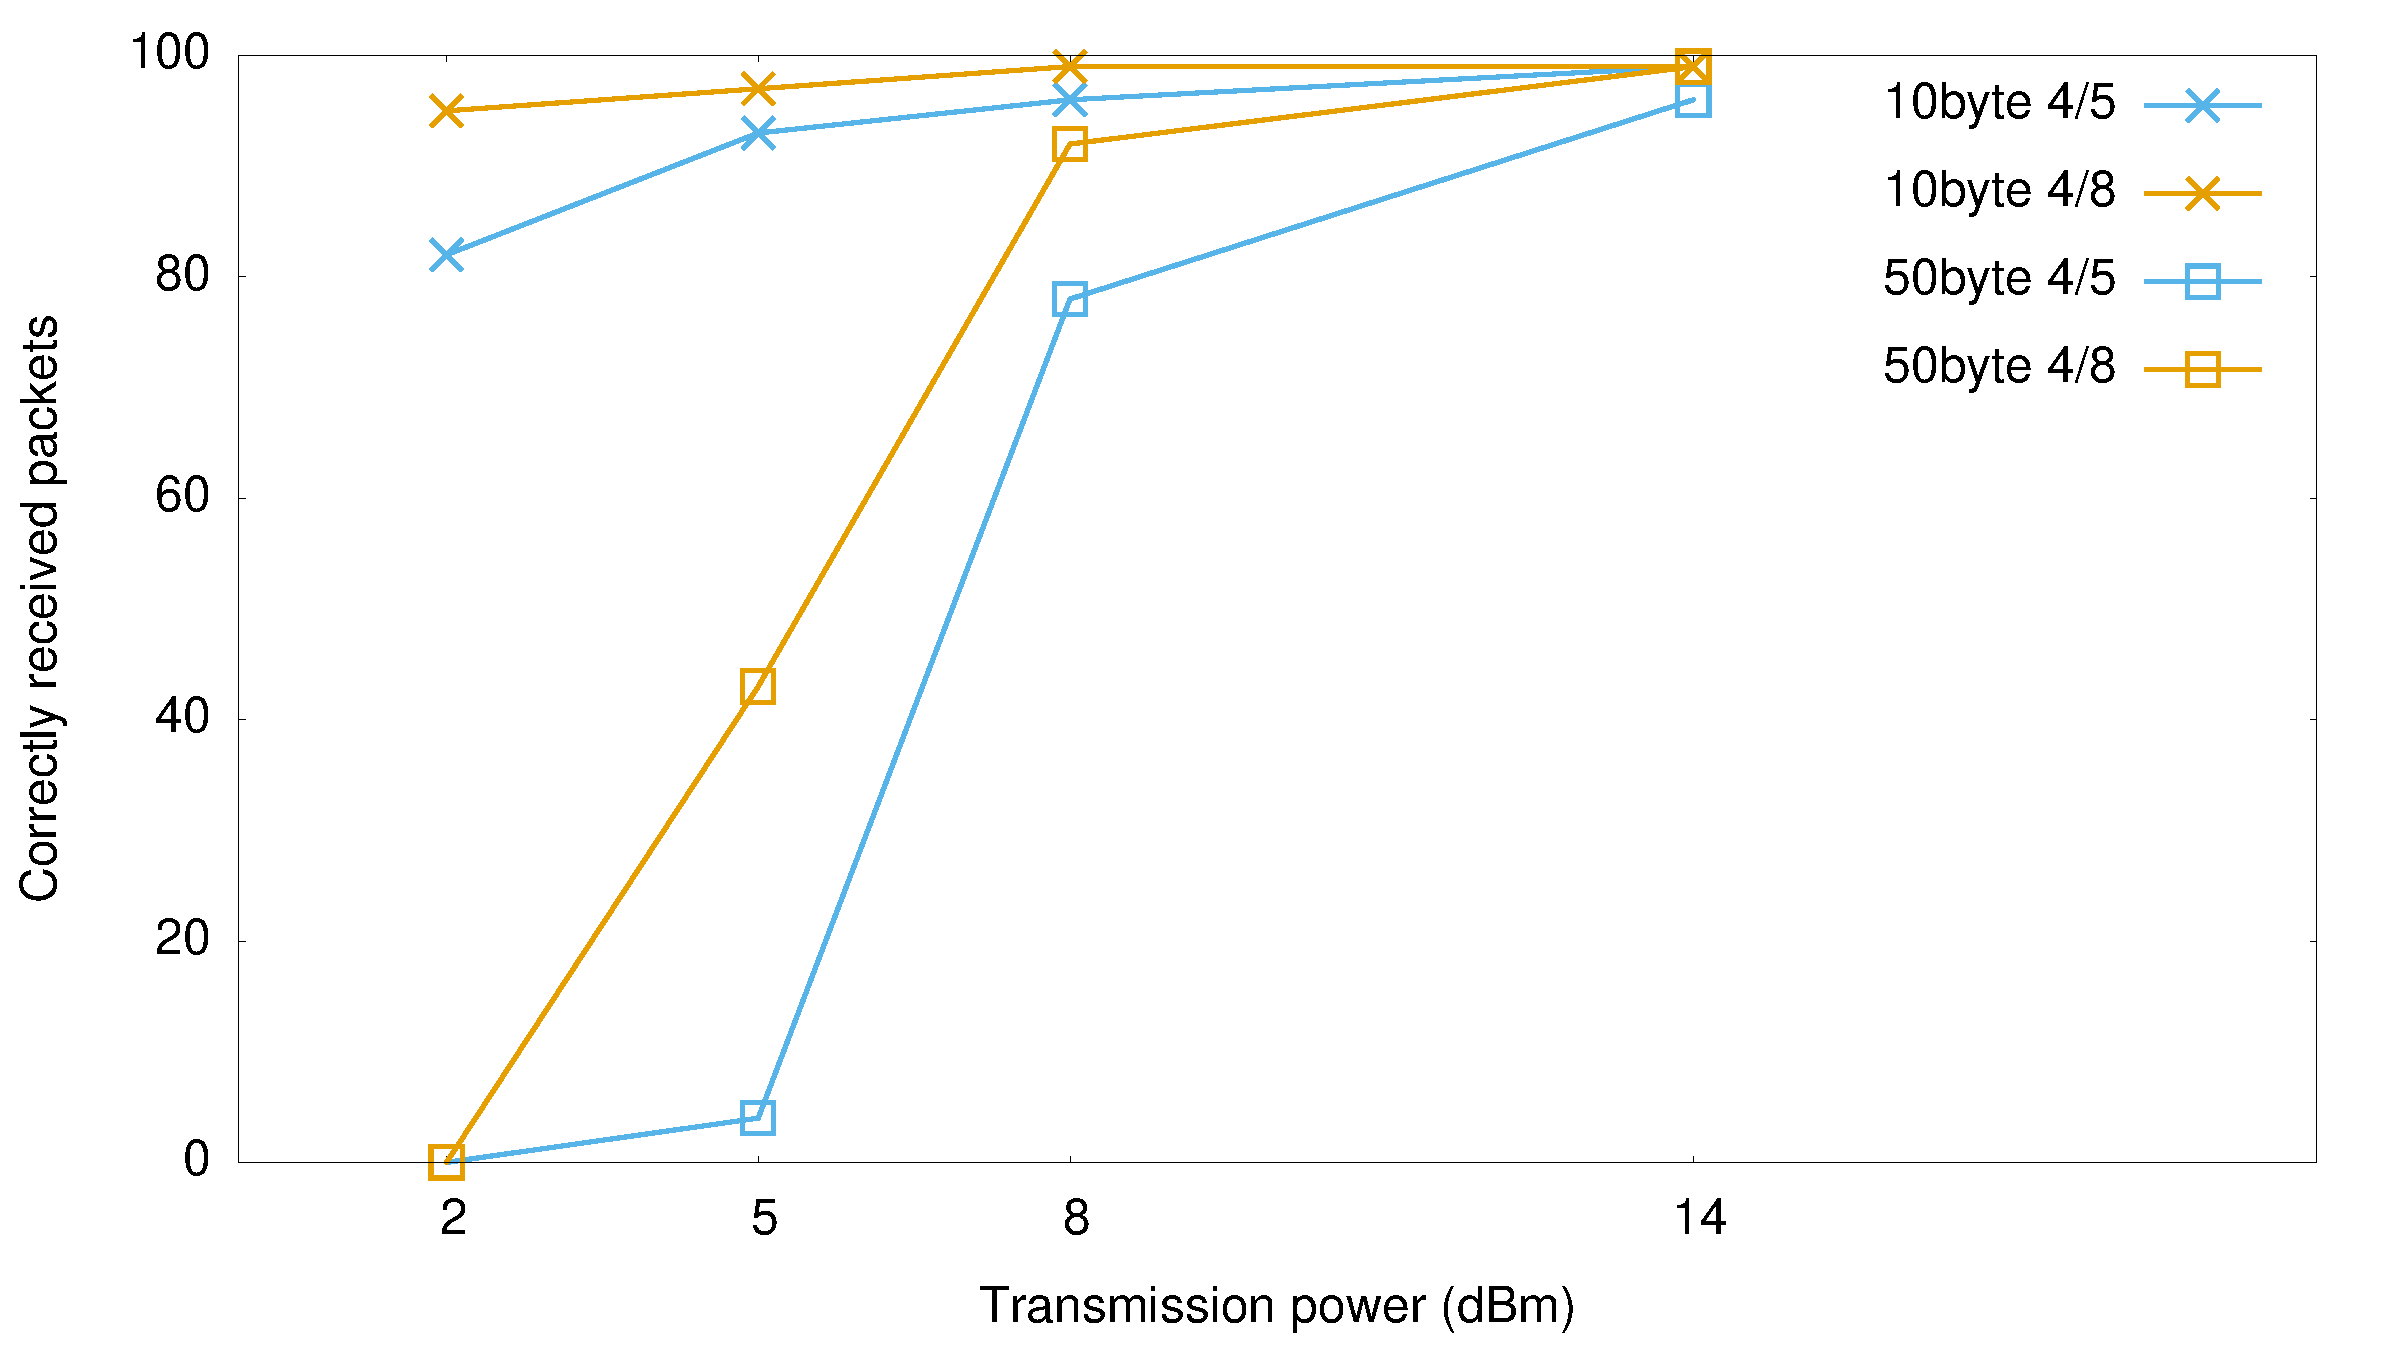
\includegraphics[width=\textwidth]{img/test/urban/sf9}
\caption{Results of urban experiments at SF 9}
\label{fig:sf9urban}
\end{figure}

\begin{figure}[]
\centering
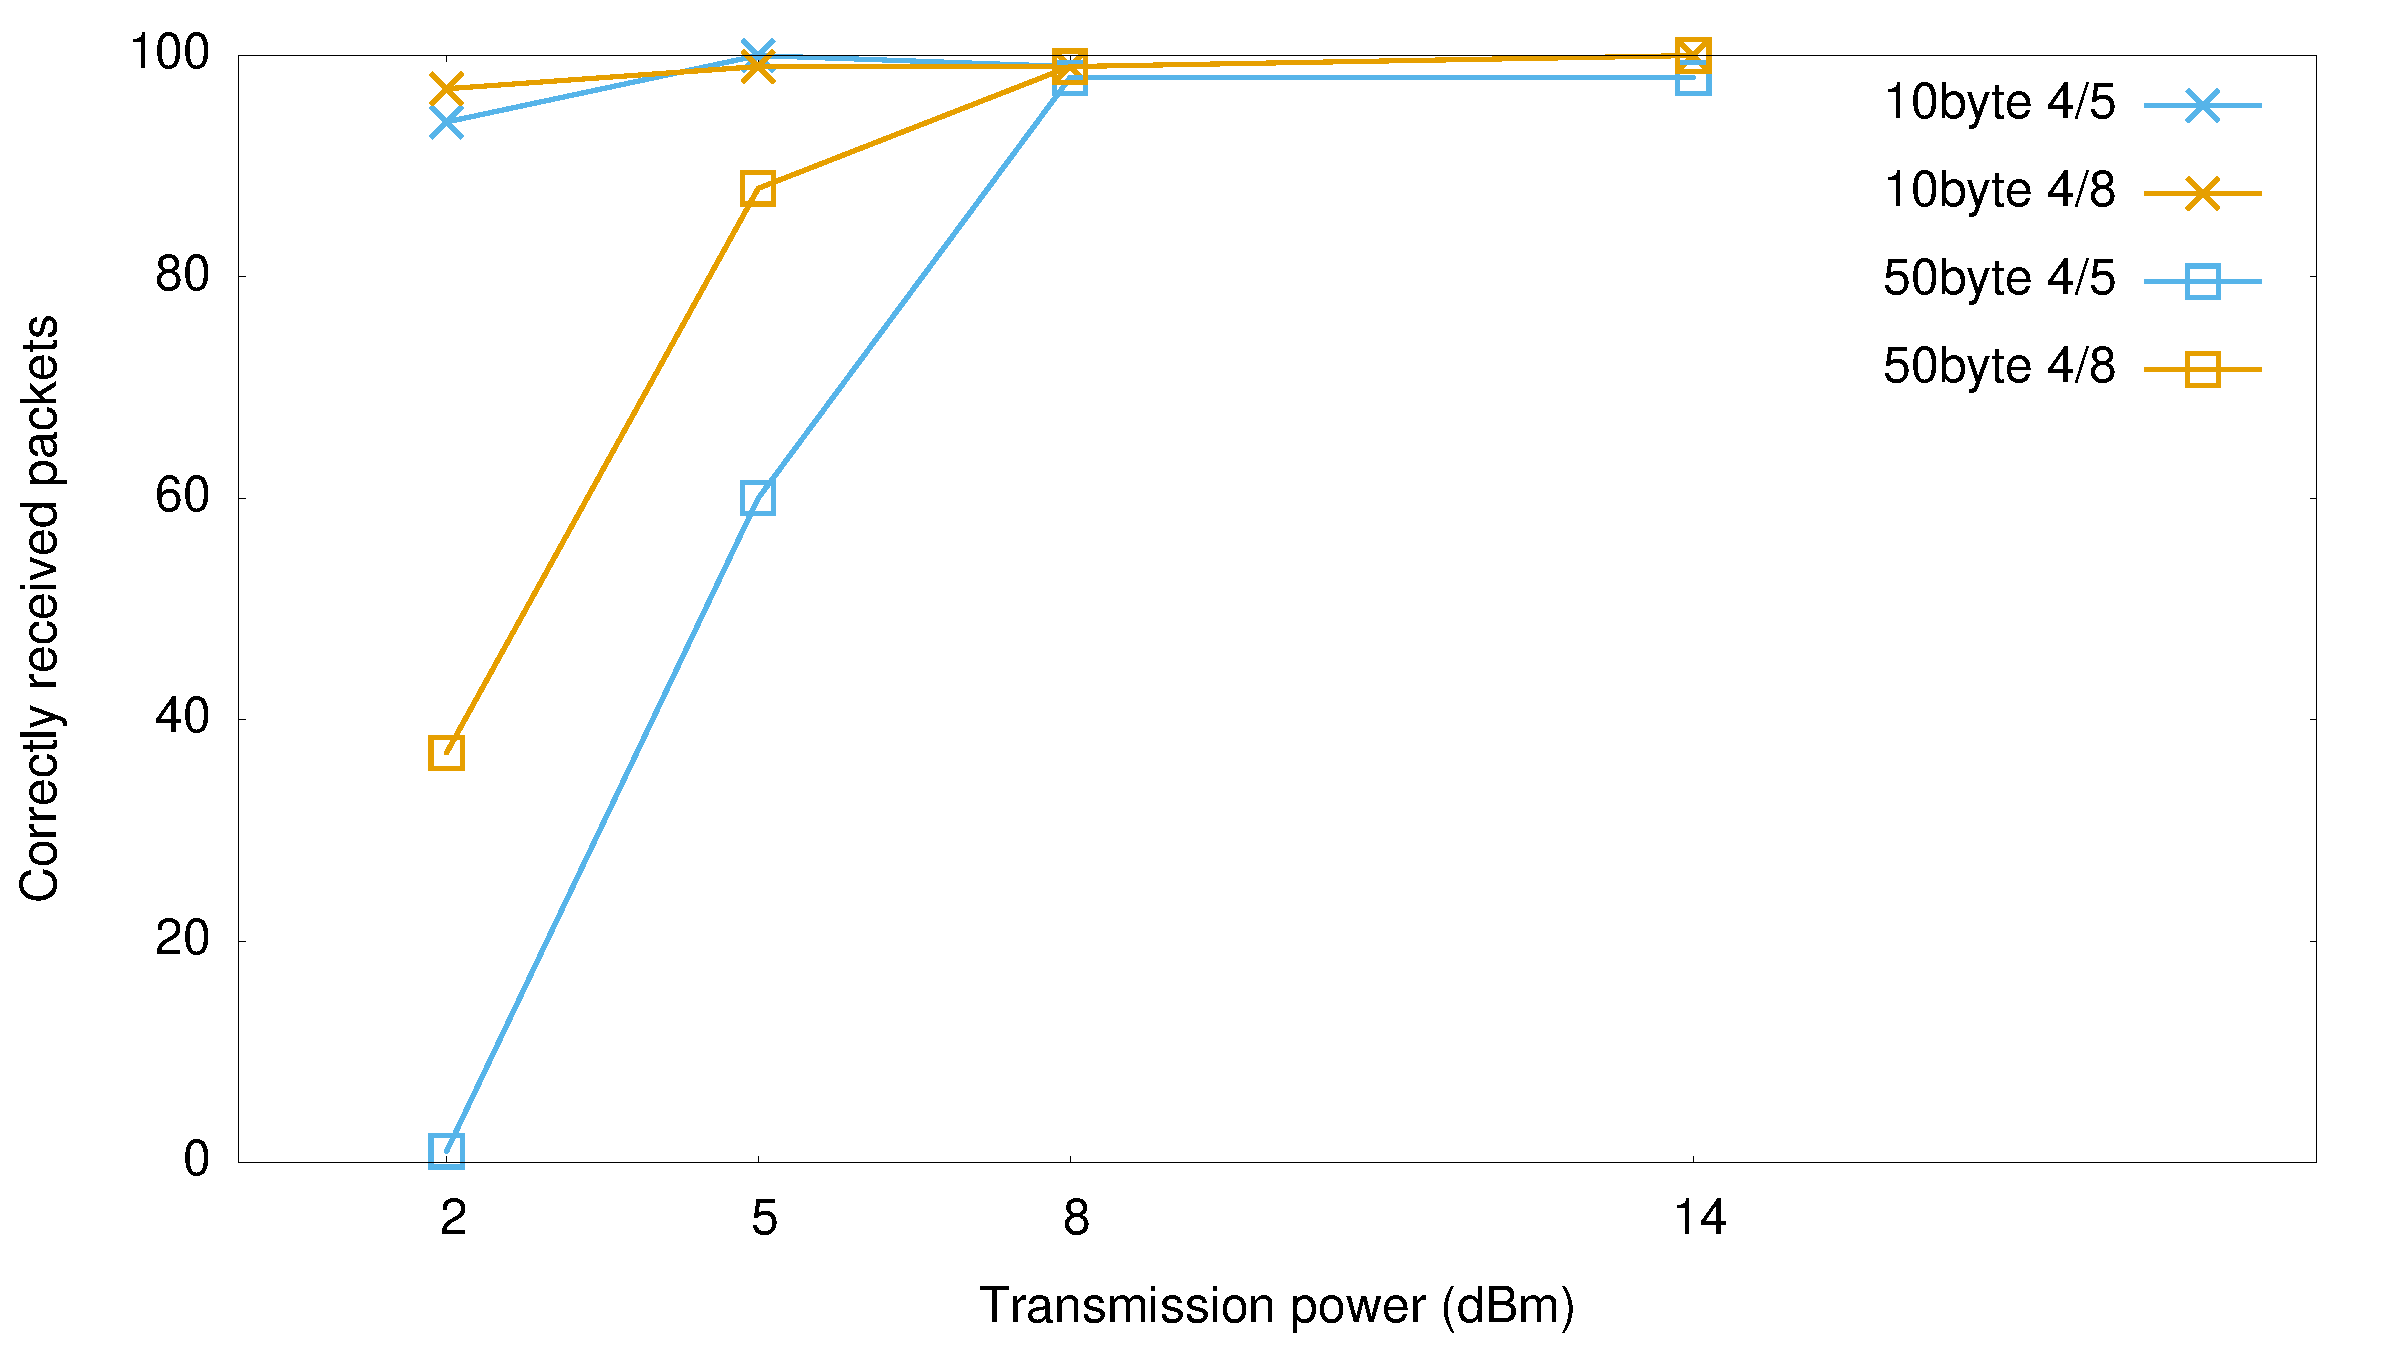
\includegraphics[width=\textwidth]{img/test/urban/sf10}
\caption{Results of urban experiments at SF 10}
\label{fig:sf10urban}
\end{figure}

\begin{figure}[]
\centering
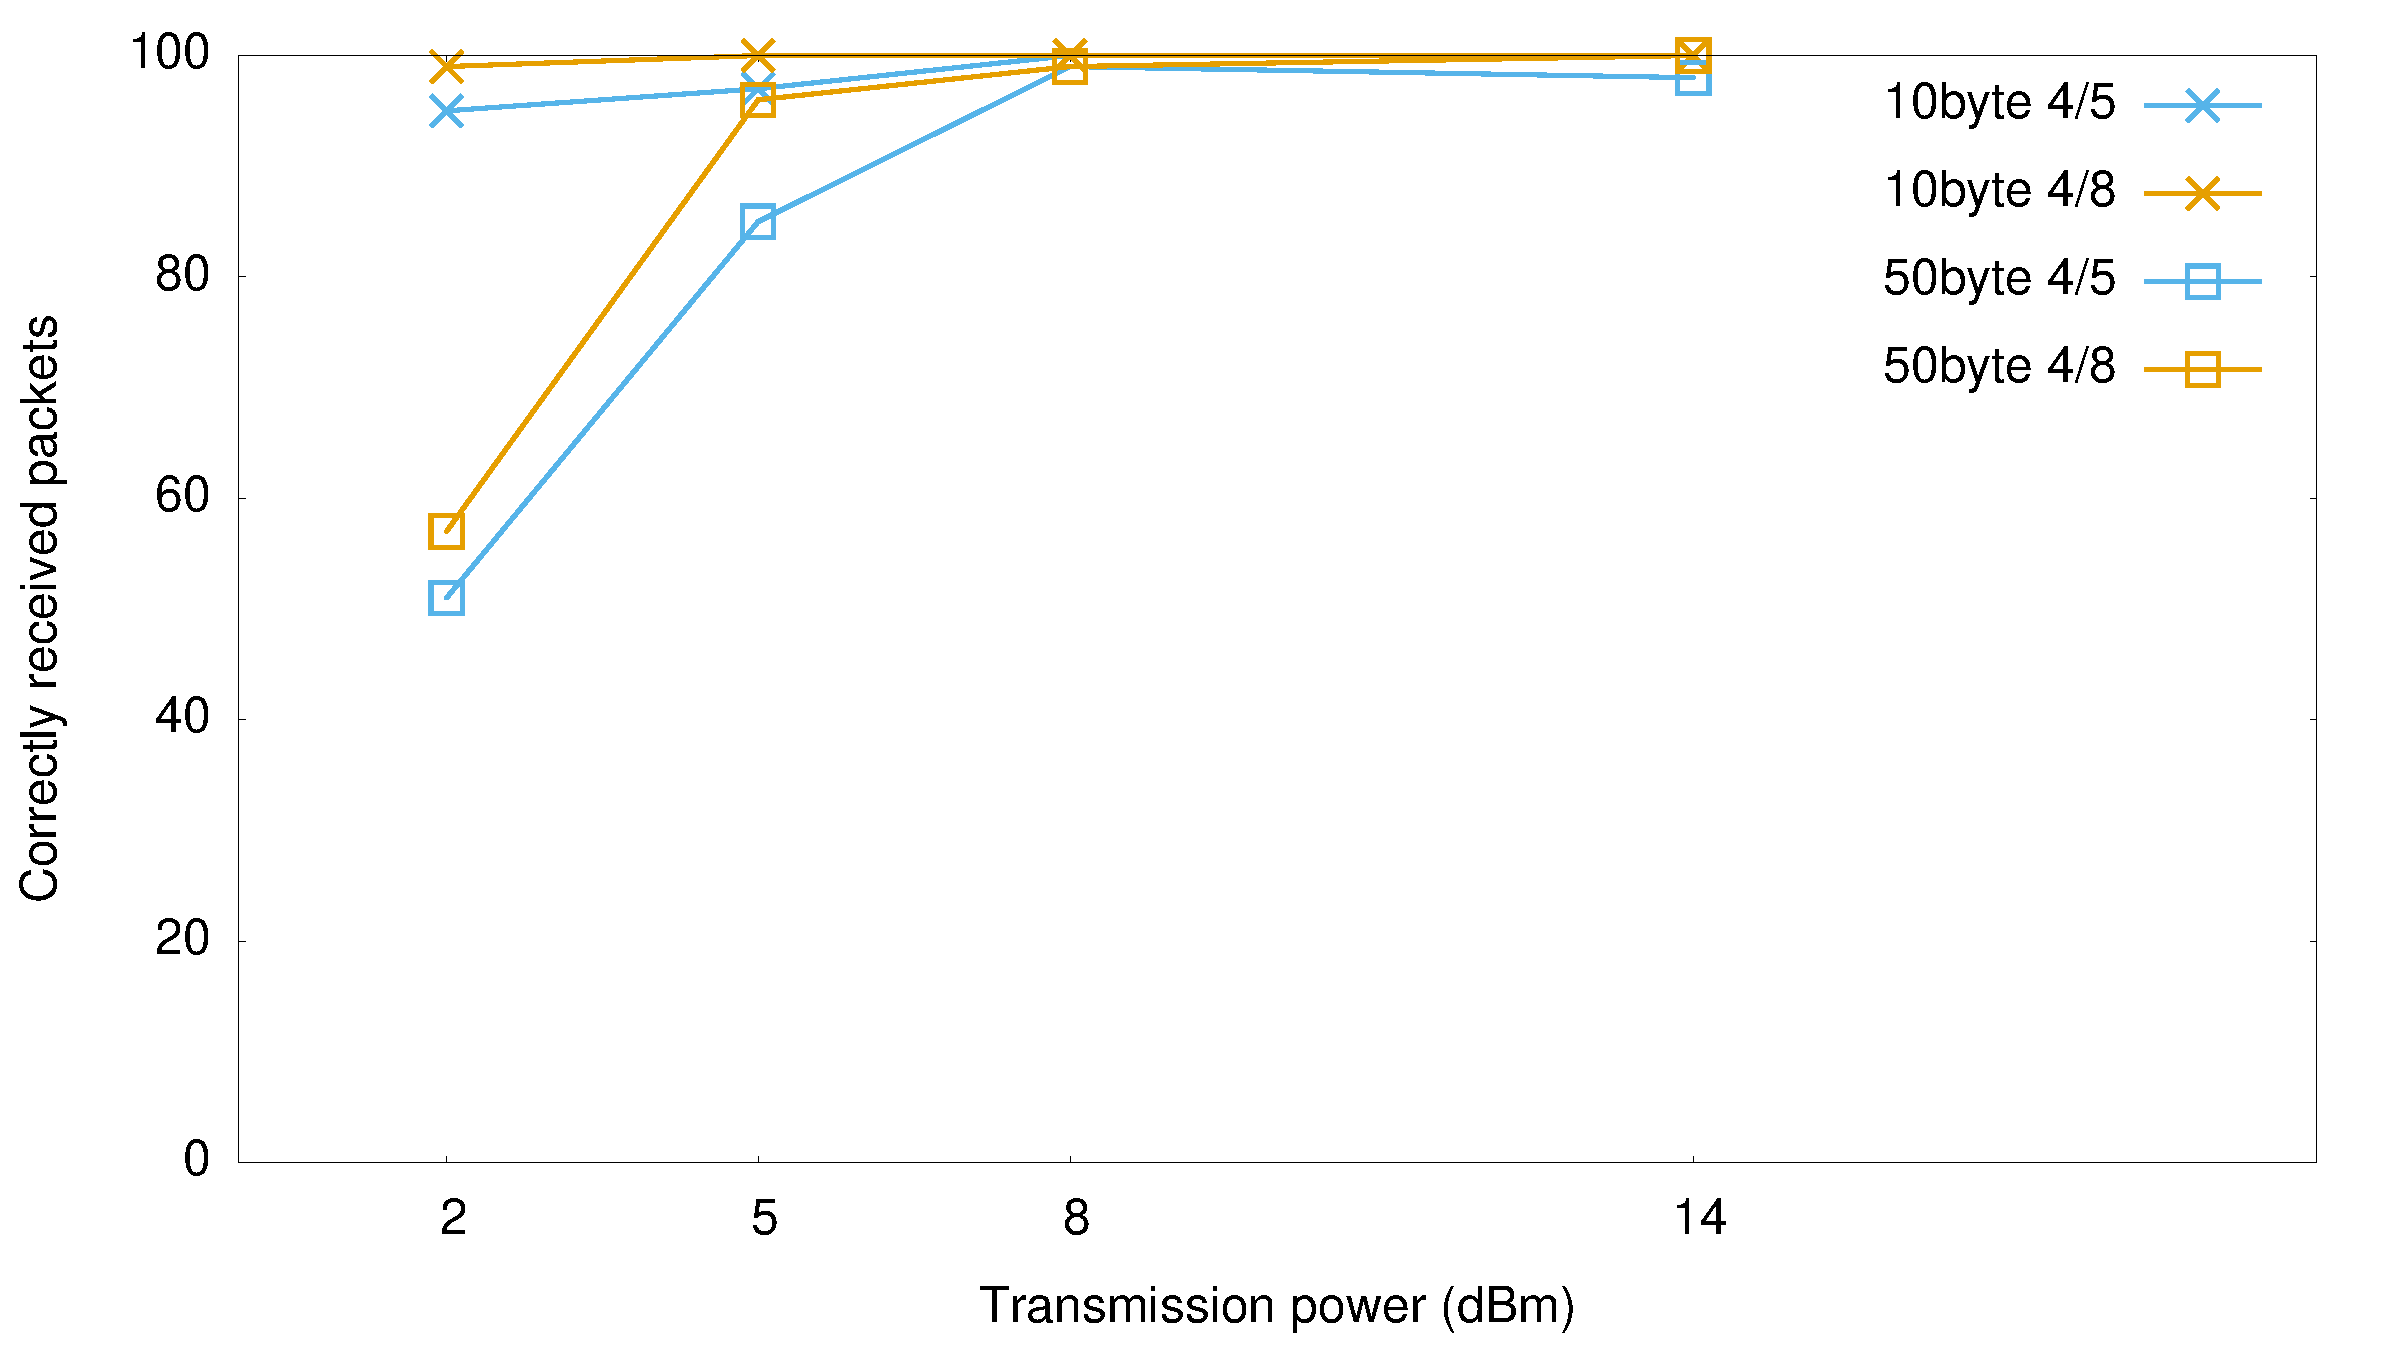
\includegraphics[width=\textwidth]{img/test/urban/sf11}
\caption{Results of urban experiments at SF 11}
\label{fig:sf11urban}
\end{figure}

\begin{figure}[]
\centering
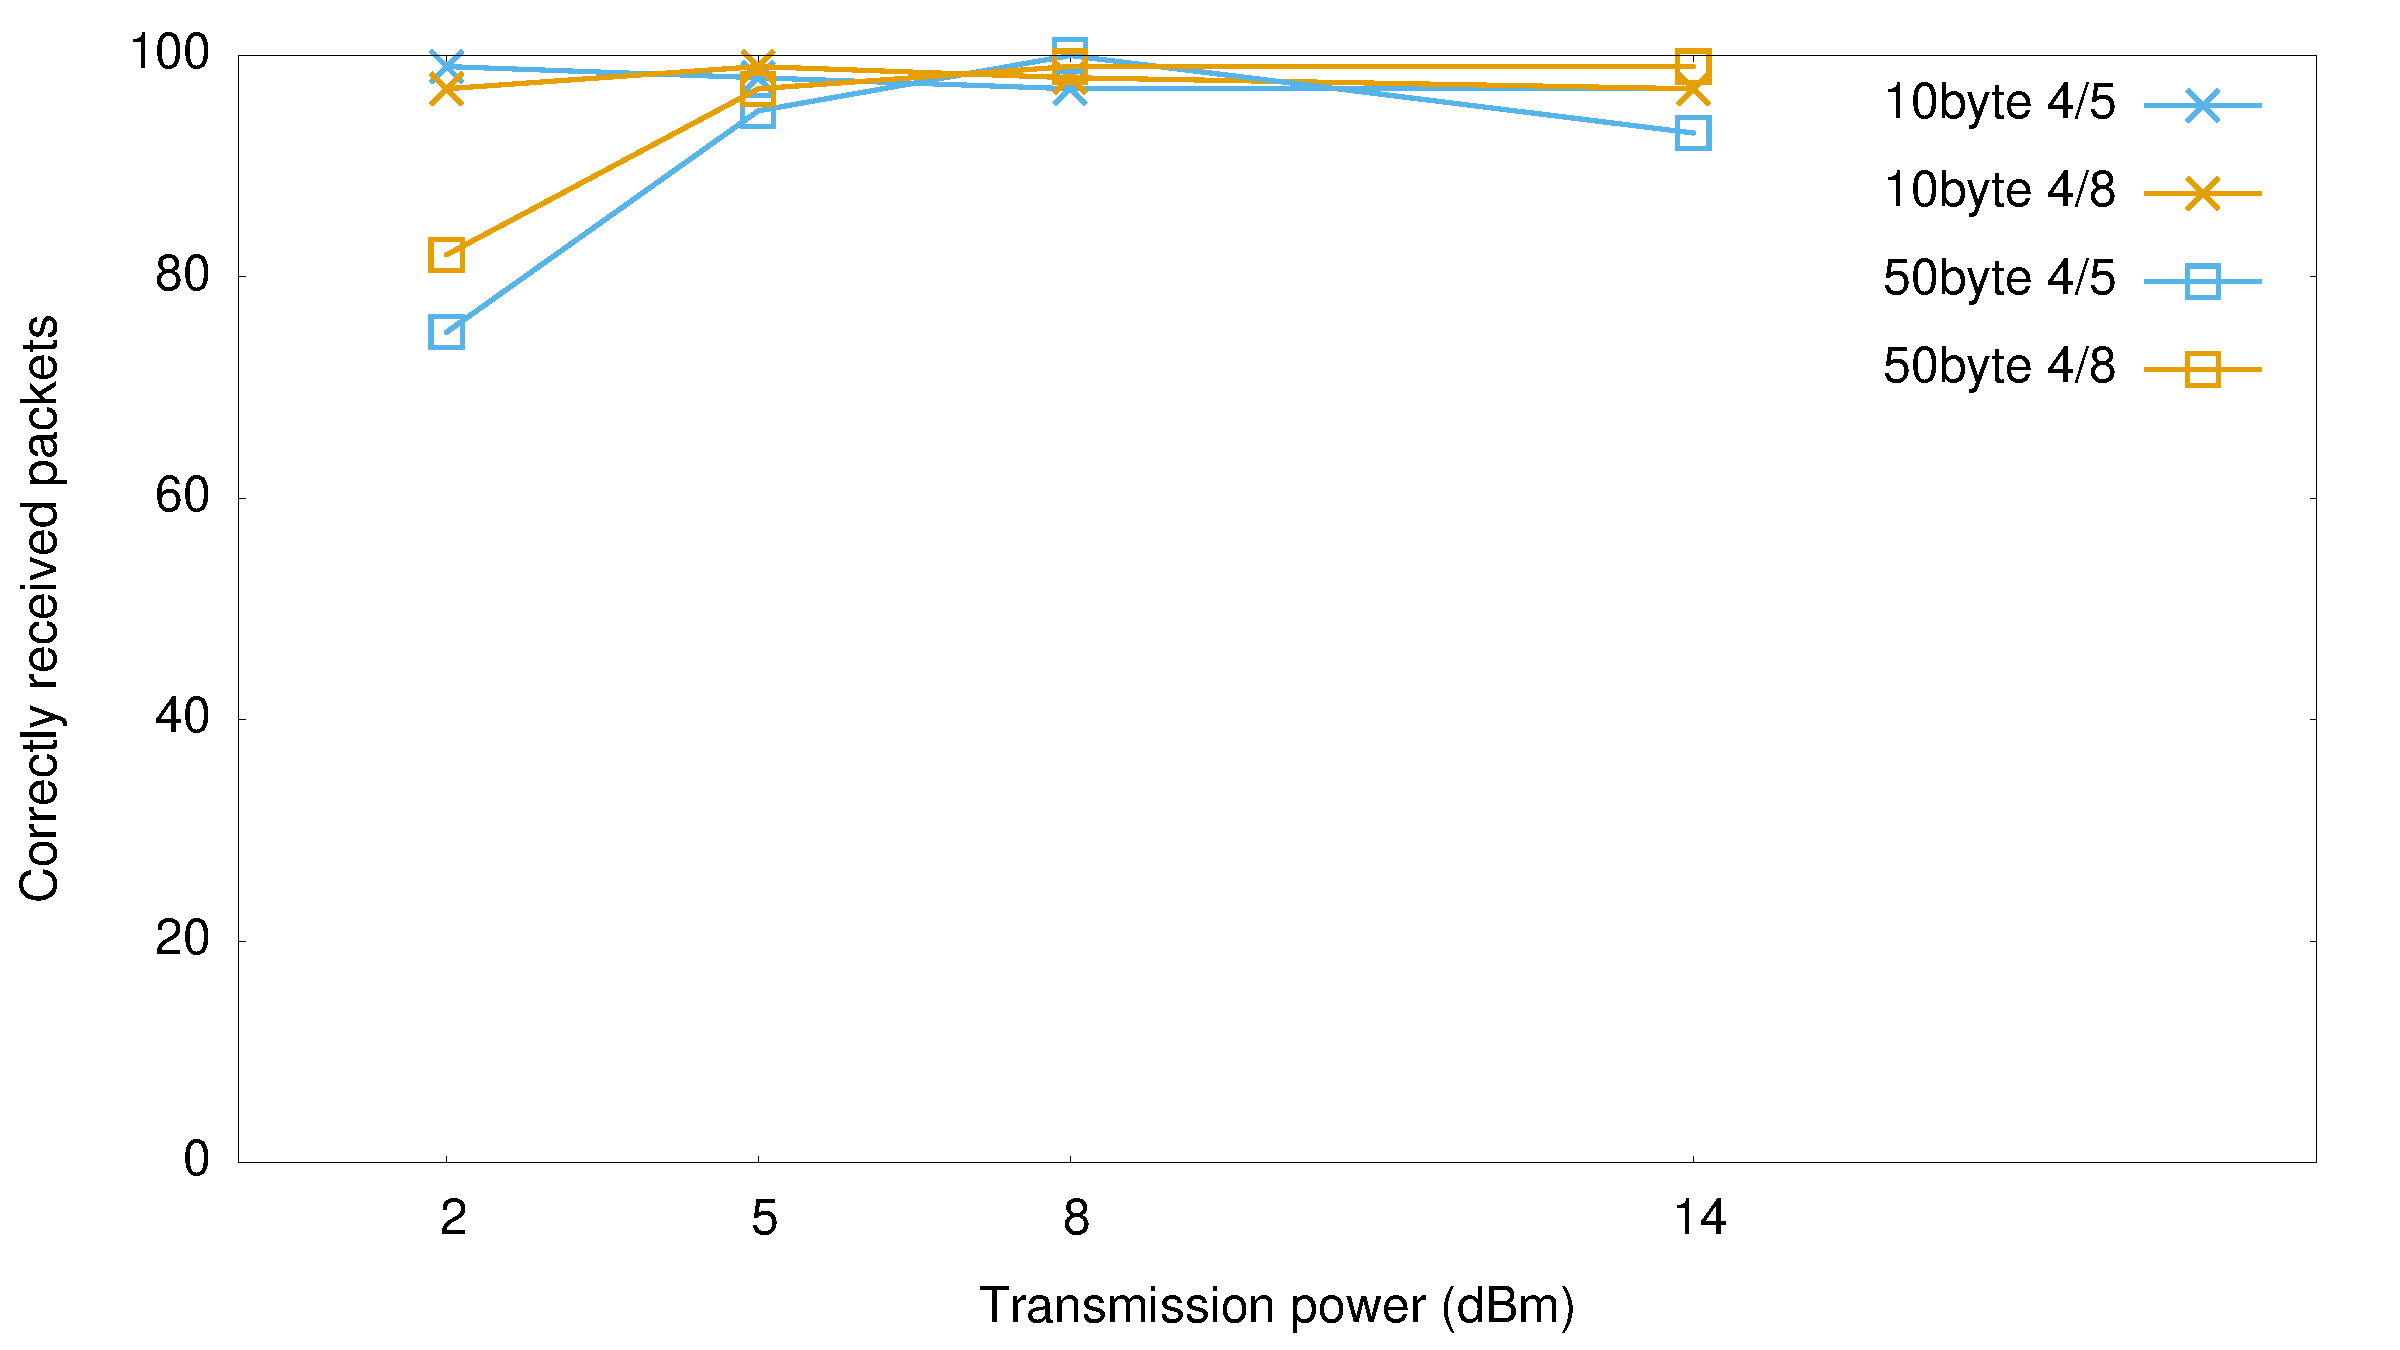
\includegraphics[width=\textwidth]{img/test/urban/sf12}
\caption{Results of urban experiments at SF 12}
\label{fig:sf12urban}
\end{figure}

\begin{figure}[]
\centering
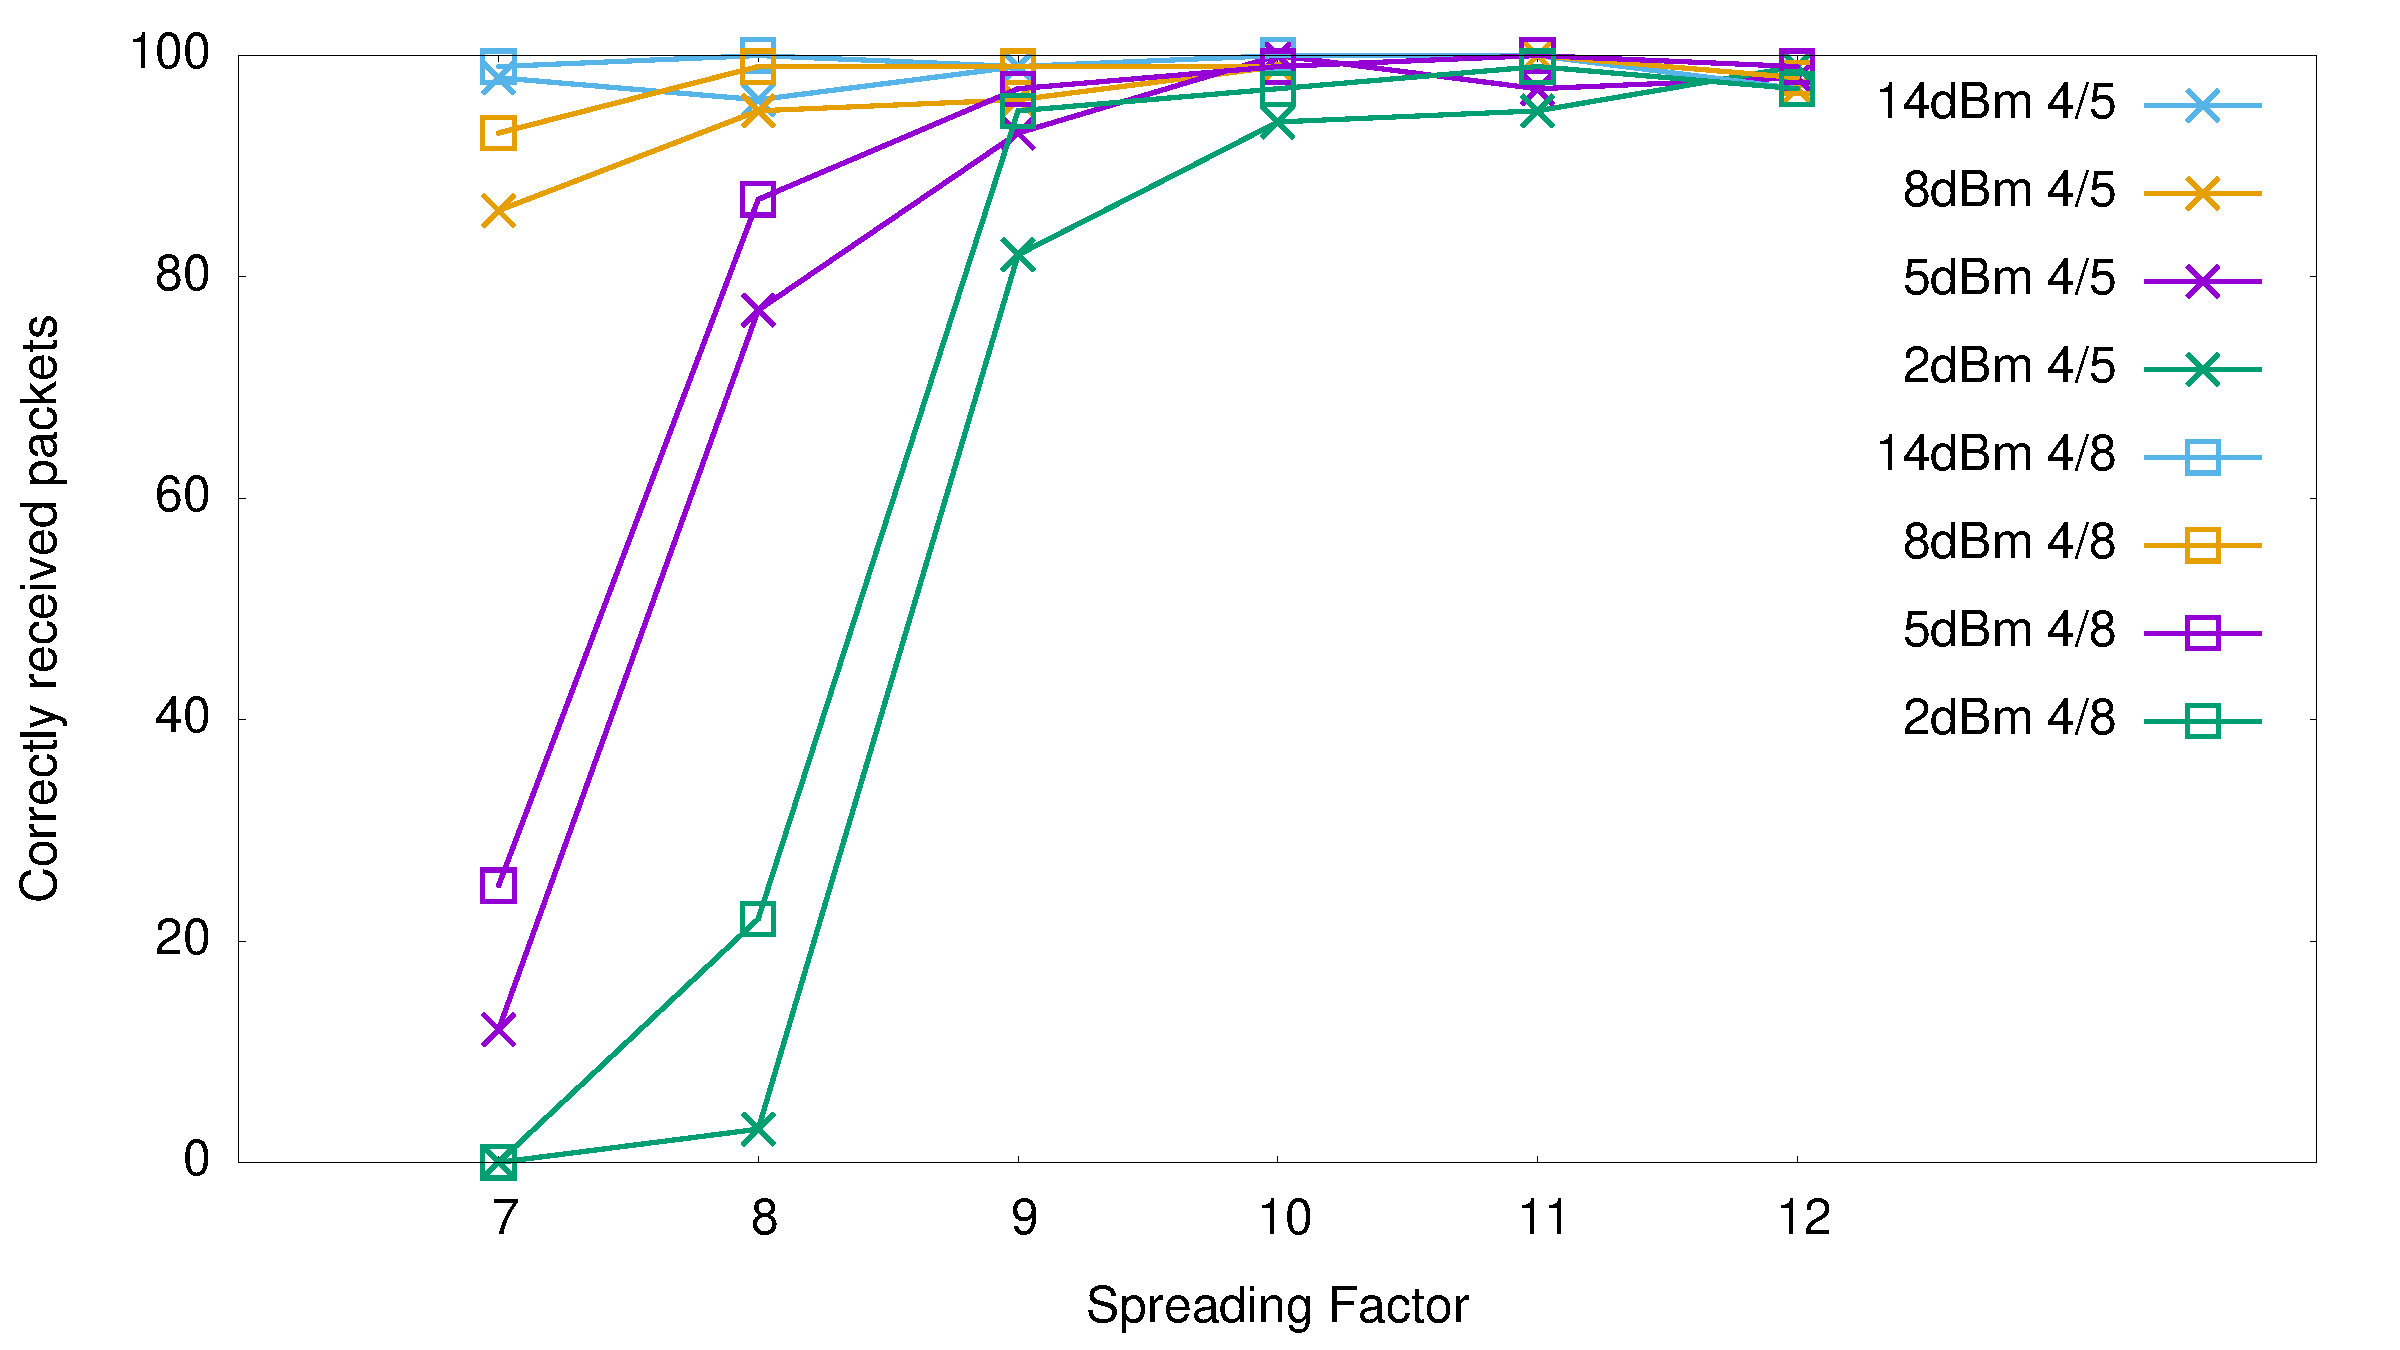
\includegraphics[width=\textwidth]{img/test/urban/len0}
\caption{Results of urban experiments with payload of 10 bytes}
\label{fig:len10urban}
\end{figure}

\begin{figure}[]
\centering
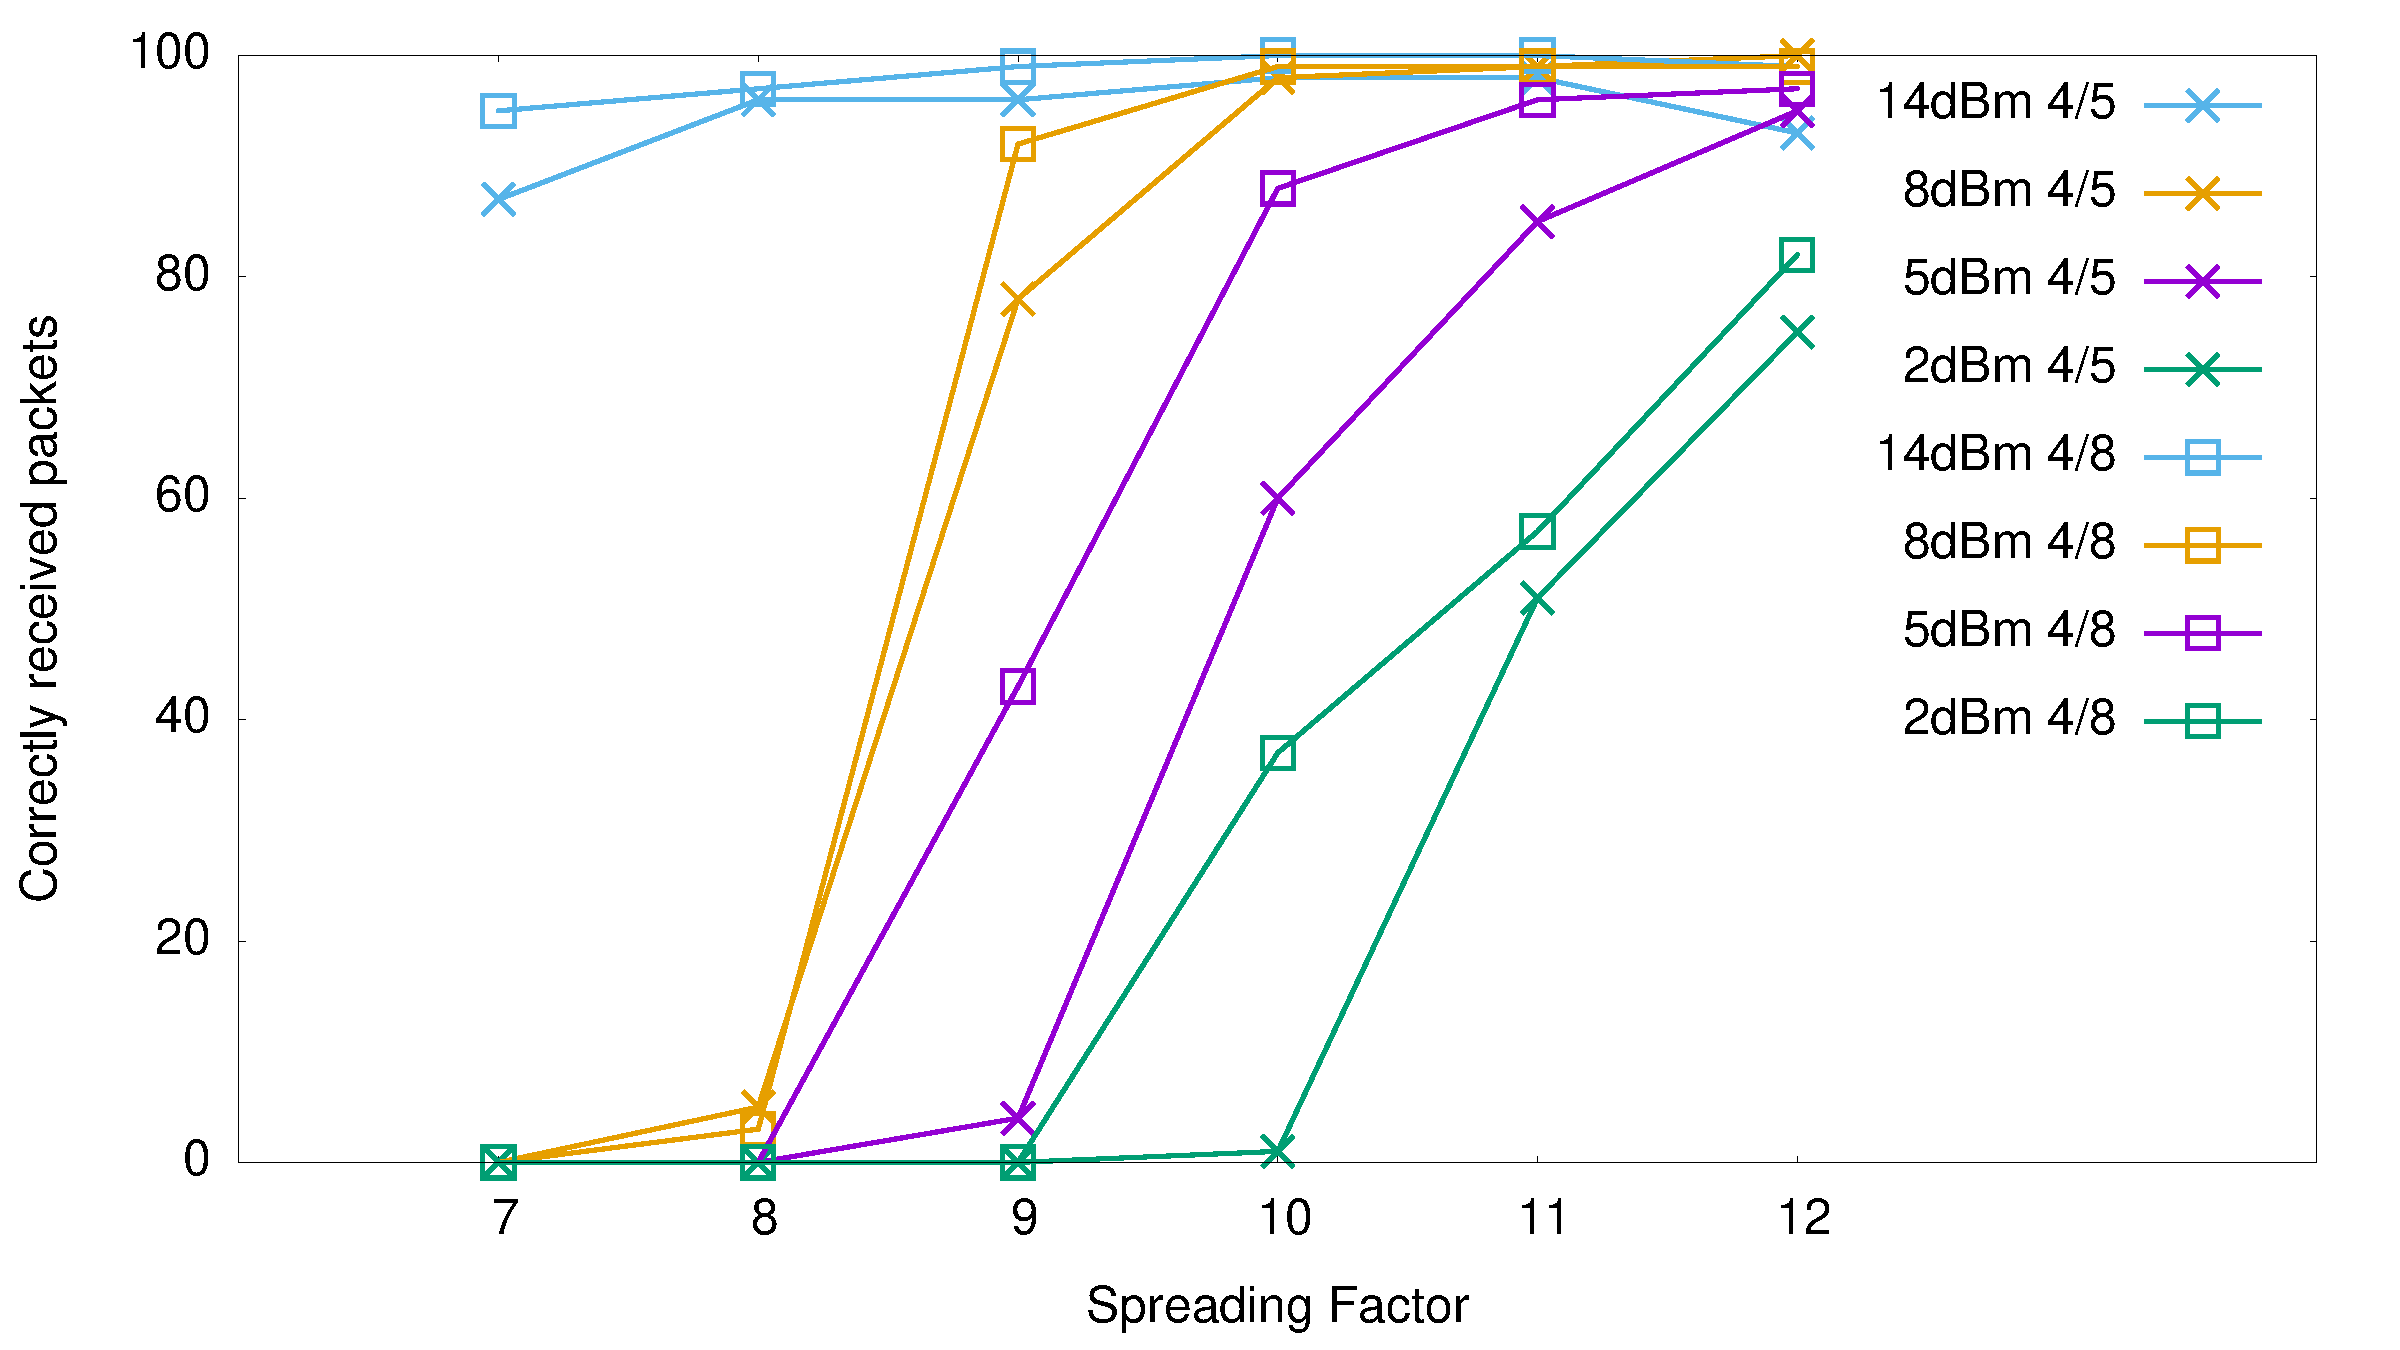
\includegraphics[width=\textwidth]{img/test/urban/len1}
\caption{Results of urban experiments with payload of 50 bytes}
\label{fig:len50urban}
\end{figure}








\chapter{LoRaWAN relay mode}
\label{chap:relayproto}

LoRaWAN networks typically are laid out in a star-of-star topology, in which end-devices communicate directly with one or more gateways, but there are many cases in which it could be useful to have a special node able to act as relay between end-devices and the gateway.

In this chapter an extension to the LoRaWAN protocol is defined, which allows the end-devices to discover and bind to any nearby relay eligible node.


\section{Motivations}

As described in chapter \ref{chap:lorawan}, the LoRaWAN protocol is designed to be deployed in a star-of-star layout, in which all the end-devices need only one LoRa communication to reach the IP network.

This architecture, of course, significantly simplifies the protocol, eliminating the need of routing mechanisms, but, on the other hand, it requires the installation of new gateways to expand the coverage area of the network.

The standard LoRa gateways, in general, require an IP connection to operate as described in the specification, and in some contexts (e.g. rural areas with no cellular coverage) it may be an impossible requirement to satisfy.

On the contrary, the solution proposed in this thesis allows to extend the coverage area without the need of gateways, and, at the same time, to increase the performances of the end-devices at the same range of coverage.


\section{Design}
\label{sec:protdesign}

\subsection{Protocol overview}

\begin{figure}
\centering
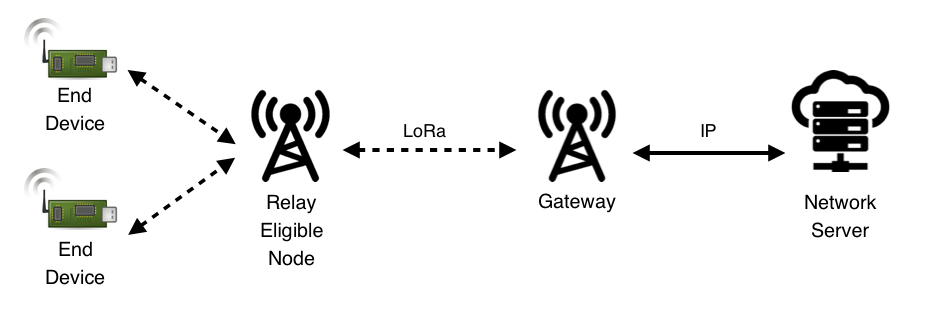
\includegraphics[width=\textwidth]{img/relay-architecture}
\caption{Reference architecture of relay mode}
\label{fig:relayarch}
\end{figure}

The main obstacle to design a relay solution in a LoRaWAN network is that the end-devices which will act as relays often have only one LoRa interface, and also the transceivers installed on these devices are not capable to open receive windows at the same time on all possible frequencies, data rates and coding rates.

With the aim to design a protocol that can be implemented on this type of end-devices it was decided to add a TDMA technique to the standard specification. The key idea is that each \emph{Relay Eligible Node} must periodically send a beacon to advertise itself to nearby end-devices. The interval of time between two beacons sent by the same relay node is called \emph{Beacon Period}. Each beacon period is divided into two different phases:

\begin{itemize}

\item \emph{Bind Phase}, in which end-devices try to bind themselves with the relay node;

\item \emph{Transmission Phase}, in which end-devices send upstream data to relay and receive downstream data.

\end{itemize}
The transmission phase is further divided into several slots, numbered starting from zero, in order to let the relay node wake up only when needed, i.e. only in proximity of slots bound to end-devices.
In each slot only one end-device is allowed to exchange data, and each end-device can transmit only in one slot per beacon period. The slot within the beacon period is assigned to the end-device by the network server in the bind phase. One slot is reserved to bind answers, and it is never assigned to devices.

\begin{figure}
\centering
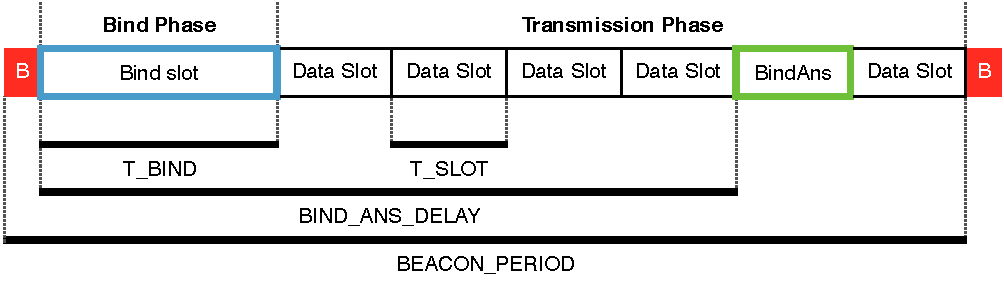
\includegraphics[width=\textwidth]{img/timing_diagram}
\caption{Timing diagram of the protocol}
\label{fig:timepdia}
\end{figure}

The beacons and all bind messages are sent using well known parameters (data rate, coding rate, frequency), which are defined in this specification. The other communications are performed using parameters which must be exchanged in bind phase.

The aim of this protocol is to extend LoRaWAN without radically changing its philosophy, so every decision is taken by the network server, which sets up both the relays and the end-devices through MAC commands.

\paragraph{Requirements} Although the very centralized nature of LoRaWAN is maintained with the new relay mode, this is not transparent to existing devices, which need to be adapted in order to support the new protocol. In particular:

\begin{itemize}
\item The end-devices must explicitly switch to relay mode;
\item The relay node must explicitly switch to relay mode, advertising its presence to neighbors and exchanging all needed parameters with the network server;
\item The network server must be update to support the new mode;
\item End-devices and relay must belong to the same network, such that they are managed by the same network server;
\end{itemize}

On the other hand, existing LoRa gateways already support the new relay mode because they do not interact with the LoRaWAN layer. Furthermore, existing standard LoRaWAN end-devices are not affected by the behavior of the updated devices. 



\paragraph{Specification} This specification includes the format of all newly defined massages and the description of the timing constraints. It can be logically divided into three parts:

\begin{itemize}
\item \emph{Relay eligible node management}: defines all the messages exchanged between the relay and the network server;

\item \emph{End-device binding}: defines all the messages exchanged in order to effectively bind (and unbind) end-devices to the relay;

\item \emph{Data transmission}: defines the protocol to adopt when an end-device wants to transmit upstream data and receive downstream data, if any.
\end{itemize}


\subsection{Relay eligible node management}

\subsubsection{Relay setup}

Before starting to advertise itself, each relay eligible node must send a \emph{RelaySetupReq} MAC command to network server, containing the minimum requirements for the parameters of the relay session.

\begin{figure}[!h]
\centering
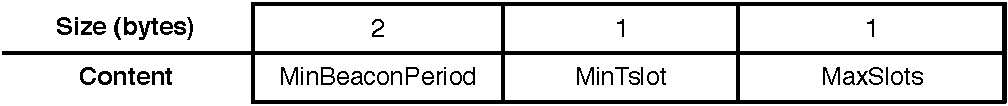
\includegraphics[width=\textwidth]{img/commands/RelaySetupReq}
\caption{RelaySetupReq MAC command}
\label{fig:relaysetupreq}
\end{figure}

In particular MinBeaconPeriod contains the minimum length of the BeaconPeriod expressed in seconds; MinTslot contains the minimum length of the slot expressed in seconds; MaxSlots contains the maximum number of slots per BeaconPeriod which the device is able to handle.

The relay node cannot advertise itself until it receives the parameters from network server through RelaySetupAns MAC command.

\begin{figure}[!h]
\centering
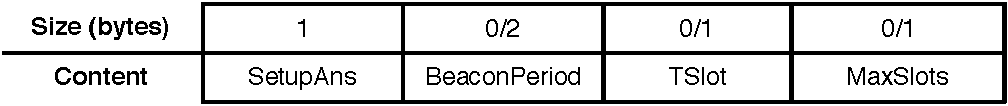
\includegraphics[width=\textwidth]{img/commands/RelaySetupAns}
\caption{RelaySetupReq MAC command}
\label{fig:relaysetupans}
\end{figure}

In particular if SetupAns equals 0x00 the device is accepted, and this field is followed by the mandatory parameters to adopt. The BeaconPeriod and the slot length TSlot are expressed in seconds. MaxSlots is the number of available slots.

If SetupAns is not equal to 0x00 the device was not accept by the network server as a relay, and it is not followed by any other fields.




\subsubsection{Relay status}
The relay may request to the network server the list of end-devices bound to it. In response it will receive the changes on the list of served end-devices from last request.
The \emph{RelayStatusReq} does not have any payload, the \emph{RelayStatusAns} has the format of figure \ref{fig:relaystatusans} and each \emph{DeviceEntry} is encoded as figure \ref{fig:deventry}

\begin{figure}[!h]
\centering
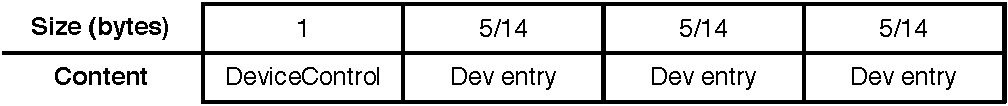
\includegraphics[width=\textwidth]{img/commands/RelayStatusAns}
\caption{RelayStatusAns MAC command}
\label{fig:relaystatusans}
\end{figure}
The \emph{DeviceControl} field (figure \ref{fig:devcontrol}) carries the \emph{ClearList} flag and the number of devices (\emph{DeviceNum}) contained into the following list.  When the \emph{ClearList} flag is set, the end-device must empty its current list before updating it with the new information contained in this MAC command.

\begin{figure}[!h]
\centering
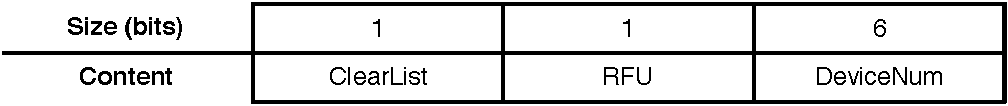
\includegraphics[width=\textwidth]{img/commands/DeviceControl}
\caption{DeviceControl field in the RelayStatusAns MAC command}
\label{fig:devcontrol}
\end{figure}

\begin{figure}[!h]
\centering
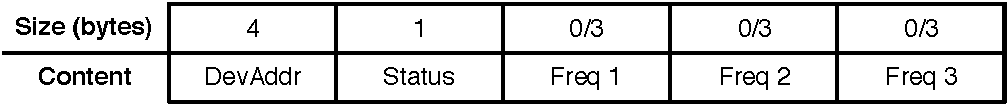
\includegraphics[width=\textwidth]{img/commands/DevEntry}
\caption{Device entry contained in RelayStatusAns MAC command}
\label{fig:deventry}
\end{figure}
The RelayStatusAns can carry as many device entry as they fit in the packet, with an upper bound of 63. Each device entry contains the address (DevAddr) and the Status of the device, which has the format described in figure \ref{fig:deventrystatus}.

\begin{figure}[!h]
\centering
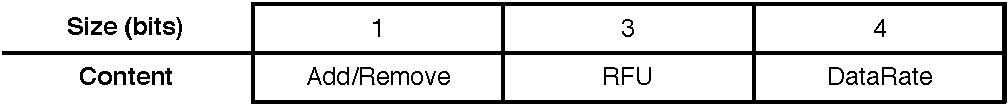
\includegraphics[width=\textwidth]{img/commands/DevEntryStatus}
\caption{Status fiend within each device entry}
\label{fig:deventrystatus}
\end{figure}

If the Add/Remove flag is set, then the relay must deallocate the slot for the end-device. Else if the Add/Remove flag is not set, then the DataRate field carries the data rate at which the end-device will transmit its messages, and the Status field is followed by 9 octets carrying the three frequencies on which the end-device will transmit.

\subsubsection{Relay stop}
The network server can stop a relay node using the \emph{RelayStopReq} MAC command. When the relay node receives the RelayStopReq command it must stop every relay activity immediately, hence the network server does not expect any answer. This command does not have any payload.


\subsection{End-device binding}
\begin{figure}[]
\centering
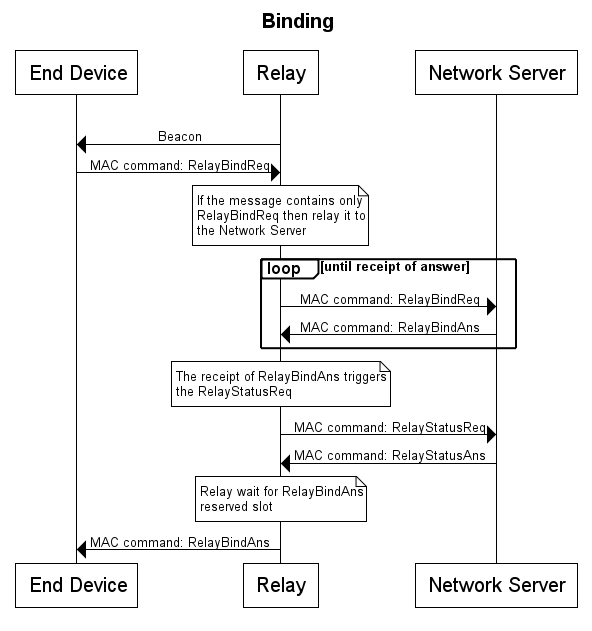
\includegraphics[width=\textwidth]{img/seqdia/binding}
\caption{Sequence diagram of the end-device binding}
\label{fig:binding}
\end{figure}

In order to bind to a relay node, the end-device starts listening to the radio channel, waiting for a beacon. If the end-device receives a beacon from a relay node it can decide either to bind to it by sending a \emph{RelayBindReq} command, or to discard the beacon and start waiting for a new one.


\subsubsection{Broadcasting Beacons}

In order to advertise its presence to its neighbors, the relay node periodically sends a beacon containing all the information needed by end-devices to set up a session with it. The beacon must be sent with the parameters reported in table \ref{tab:beaconparams}.


% Please add the following required packages to your document preamble:
% \usepackage{booktabs}
\begin{table}[]
\centering
\caption{Transmission parameters of the beacon}
\label{tab:beaconparams}
\begin{tabular}{@{}ll@{}}
\toprule
\multicolumn{1}{c}{Parameter} & \multicolumn{1}{c}{Value} \\ \midrule
Data Rate                     & SF9 BW125                 \\
Coding Rate                   & 4/5                       \\
Frequency                     & 869.525 MHz               \\
Period                        & BEACON\_PERIOD            \\ \bottomrule
\end{tabular}
\end{table}



\begin{figure}[!h]
\centering
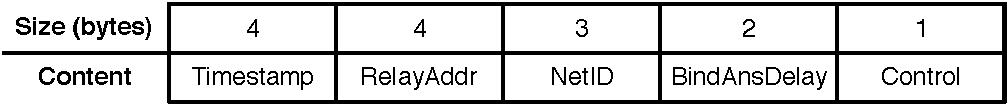
\includegraphics[width=\textwidth]{img/Beacon}
\caption{Beacon format}
\label{fig:beacon}
\end{figure}


Relay must include in the beacon its address (RelayAddr) and the ID of the network (NetID) to which it belongs to, in order to let the end-device select only relays belonging to its own network. The NetID has the format described in the LoRaWAN specifications. The Timestamp field contains the internal timestamp of the relay node, using milliseconds unit of measure. The Control field contains RFU flags.



\subsubsection{RelayBindReq}

The bind request must be sent only in the bind slot, and exactly RX\_DELAY seconds after the end of the beacon transmission. The bind request must be performed using MAC command RelayBindReq, which has the format shown in figure \ref{fig:relaybindreq}.

\begin{figure}[!h]
\centering
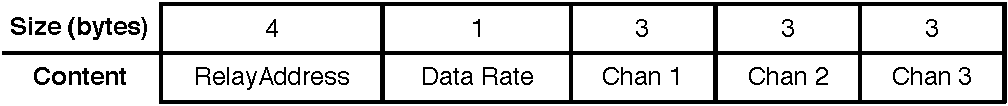
\includegraphics[width=\textwidth]{img/commands/RelayBindReq}
\caption{RelayBindReq MAC command}
\label{fig:relaybindreq}
\end{figure}

These parameters are used by the relay to open the receive window at the beginning of the transmission slot. Each \emph{Chan} field contains the center frequency of the channel, expressed in Hertz and divided by 100. For instance, if the center frequency of the channel is 868300000 Hz, the corresponding \emph{Chan} field into the RelayBindReq will contain the number 8683000.

The \emph{DataRate} field is encoded as shown in figure \ref{fig:datarate}.

\begin{figure}[!h]
\centering
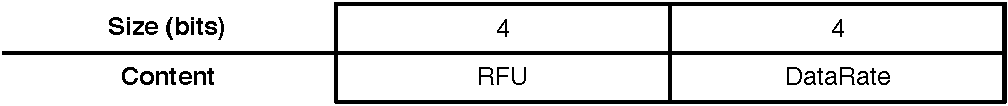
\includegraphics[width=\textwidth]{img/commands/DataRate}
\caption{DataRate field into RelayBindReq MAC command}
\label{fig:datarate}
\end{figure}

\subsubsection{RelayBindAns}
Network server must answer to a RelayBindReq with a RelayBindAns MAC command, which has the format shown in figure \ref{fig:relaybindans}.

\begin{figure}[!h]
\centering
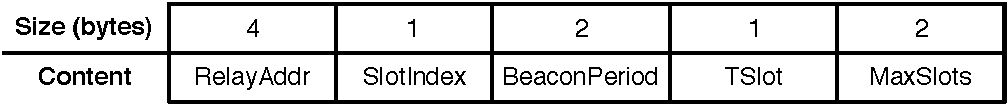
\includegraphics[width=\textwidth]{img/commands/RelayBindAns}
\caption{RelayBindAns MAC command}
\label{fig:relaybindans}
\end{figure}

The recipient of a RelayBindAns MAC command is the end-device who has sent the RelayBindReq. The network server must include in the RelayBindAns MAC command the following information:

\begin{description}
\item[RelayAddr] the address of the relay;
\item[SlotIndex] index of the time slot assigned to the device;
\item[BeaconPeriod] time-interval between two beacons, expressed in seconds;
\item[TSlot] time slot length, expressed in seconds;
\item[MaxSlots] number of slots within one beacon period.
\end{description}
The end-device will receive the RelayBindAns MAC command into the \emph{BindAns} slot, which is advertised within the beacon through the field \emph{BindAnsDelay}. If the RelayBindAns MAC command is not received in the first available BindAns slot, the original RelayBindReq must be considered lost and the end-device must perform a new bind request.

\subsubsection{RelayUnbindReq}

\begin{figure}[!h]
\centering
\includegraphics[width=\textwidth]{img/seqdia/unbinding}
\caption{Sequence diagram of the end-device unbinding}
\label{fig:unbinding}
\end{figure}

The end-device may explicitly unbind from its relay by sending a \emph{RelayUnbindReq} MAC command to the network server, which reacts de-allocating the time slot reserved to the end-device starting from the next beacon period. The RelayUnbindReq contains only the command identifier without parameters.

The network server may also autonomously detect the unbinding of the end-device, considering the device unbound after \emph{MAX\_EMPTY\_SLOTS} slots without receiving data from the end-device. So, in order to keep the session alive, the end-device must send an upstream message at least every MAX\_EMPTY\_SLOTS / 2 slots.

The end-device may use the the \emph{LinkCheckReq} MAC command to detect the unbinding. If after \emph{MAX\_LINK\_CHECK\_REQUESTS} the end-device does not receive any \emph{LinkCheckAns}, it considers itself unbound.




\subsection{Data transmission}
Each client is allowed to send upstream messages only within its own slot, using the previously agreed channel parameters.

\begin{figure}[]
\centering
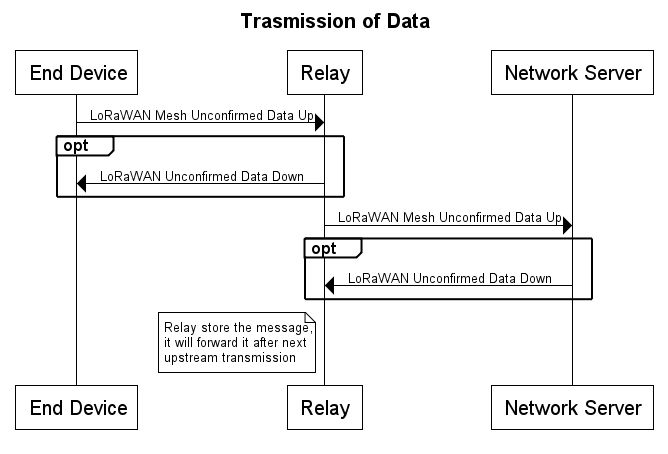
\includegraphics[width=\textwidth]{img/seqdia/datatx}
\caption{Sequence diagram of the data transmission}
\label{fig:datatx}
\end{figure}



\subsubsection{Communication between end-device and relay}
\paragraph{Channel selection}
During bind phase the client node must include into the \emph{RelayBindReq} command three channel definitions to use in transmission phase. Both the client and the relay must cycle on list of channels in the order they are defined in the \emph{RelayBindReq}, so at the first available slot after binding both devices must use the first channel defined, then they must loop on the list of channels. 

\paragraph{Message type}
Each end-device operating in relay mode must tag its messages in order to let the network server distinguish between directly sent messages and relayed ones. This can be done introducing new message type called \emph{Mesh Unconfirmed Data Up} (type 110). 
All upstream messages sent by an end-device will have Mesh Unconfirmed Data Up as type, and they will not be acknowledged by the network server.
When a network server receive a Mesh Unconfirmed Data Up message, it should discard all the statistics collected by the gateway (e.g. RSSI) because the device who has transmitted the message to the gateway, i.e. relay, is not the device indicated in the DevAddress field, i.e. the end-device.


\subsubsection{Communication between relay and gateway}
The communication between the relay node and the gateway follows the LoRaWAN 1.0 specification, except for the fact that all upstream message have the newly defined Mesh Unconfirmed Data Up as message type.
Given that relay forwards exactly the LoRaWAN message it has received, it may receive an answer form the network server which will have ClientAddr as DestAddr. The relay node must store the message until next transmission form the end-device, than it must forward it.


\subsection{MAC Commands and parameters}
As already stated, all the set up information between end-devices, relay and network server are exchanged by means of MAC commands. The new MAC commands defined in this protocol are summarized in table \ref{tab:commands}.

% Please add the following required packages to your document preamble:
% \usepackage{booktabs}
% \usepackage{multirow}
\begin{table}[]
\centering
\caption{MAC commends}
\label{tab:commands}
\begin{tabular}{@{}llcccl@{}}
\toprule
\multicolumn{1}{c}{\multirow{2}{*}{CID}} & \multicolumn{1}{c}{\multirow{2}{*}{Command}} & \multicolumn{3}{c}{Transmitted by} & \multicolumn{1}{c}{\multirow{2}{*}{Description}}                                                                               \\
\multicolumn{1}{c}{}                     & \multicolumn{1}{c}{}                         & ED        & Relay       & NS       & \multicolumn{1}{c}{}                                                                                                           \\ \midrule
0x80                                     & RelaySetupReq                                &           & x           &          & \begin{tabular}[c]{@{}l@{}}Requests parameters to start\\ acting as a relay, attaching\\ the minimum requirements\end{tabular} \\ \midrule
0x81                                     & RelaySetupAns                                &           &             & x        & \begin{tabular}[c]{@{}l@{}}Answer to RelaySetupReq,\\ with the requested parameters\end{tabular}                               \\ \midrule
0x82                                     & RelayStatusReq                               &           & x           &          & \begin{tabular}[c]{@{}l@{}}Requests the network server\\ to send changes on bound\\ end-devices\end{tabular}                   \\ \midrule
0x83                                     & RelayStatusAns                               &           &             & x        & \begin{tabular}[c]{@{}l@{}}List of new end-devices or\\ “clear list” command\end{tabular}                                      \\ \midrule
0x84                                     & RelayStopReq                                 &           &             & x        & Requests the relay to stop                                                                                                     \\ \midrule
0x85                                     & RelayBindReq                                 & x         &             &          & Requests to bind to a relay                                                                                                    \\ \midrule
0x86                                     & RelayBindAns                                 &           &             & x        & Answer to RelayBindReq                                                                                                         \\ \midrule
0x87                                     & RelayUnbindReq                               & x         &             &          & \begin{tabular}[c]{@{}l@{}}Notifies the network server\\ the unbinding of an end-device\end{tabular}                           \\ \bottomrule
\end{tabular}
\end{table}


The value of each parameter is not fixed into the specification, but it can be determined upon installation according to the use case. In table \ref{tab:params} there are some tested parameters.


% Please add the following required packages to your document preamble:
% \usepackage{booktabs}
\begin{table}[]
\centering
\caption{Parameters}
\label{tab:params}
\begin{tabular}{@{}ll@{}}
\toprule
\multicolumn{1}{c}{Constant} & \multicolumn{1}{c}{Value} \\ \midrule
BEACON\_PERIOD               & 300 s                     \\
RX\_DELAY                    & 1 s                       \\
MAX\_LINK\_CHECK\_REQUESTS   & 10                        \\
MAX\_EMPTY\_SLOTS            & 20                        \\
T\_BIND                      & 30 s                      \\
T\_SLOT                      & 10 s                      \\
MAX\_SLOTS                   & 28                        \\ \bottomrule
\end{tabular}
\end{table}






\section{Implementation}

The \emph{Waspmote Pro} is a model of mote produced by Libelium and designed for the Internet of Things. It consists of a small board which includes an ATmega 1281 microcontroller, some analog and digital I/O pins, one socket for the GPS module and two sockets for the radio modules. The latter can be used to install on the Waspmote Pro transceivers for different radio technologies like Zigbee, Wi-Fi, Sigfox and LoRaWAN.

Each transceiver implements in hardware the network protocol for which it was designed, and it gives access to its features through a limited set of APIs. The philosophy behind these design choices is that the transceiver is responsible for the correct implementation of the network protocol, especially for the timing constraints, so each update of the network protocol involves the redesign of the radio module.

Since there was not the possibility of producing a new transceiver updated to the specifications described in section \ref{sec:protdesign}, it was decided to implement a subset of the protocol in software, introducing minor changes in order to overcome the inability to operate directly at the physical level.

In particular, the limitations of the platform that do not allow the full implementation of the protocol in software are the following:

\begin{itemize}
\item Single thread programming: the standard Waspmote Pro SDK does not allow to create multi-thread applications;

\item Granularity of power saving mode: the APIs allow to enter power saving mode with the granularity of seconds, so to have more precision it is necessary to use busy wait;

\item Impossibility to synchronize the internal clock with other motes without using the GPS module;

\item Synchronous APIs with varying lengths of time between send and receive calls. Since the synchronization between two nodes is done taking as reference point the instant at which ends the transmission of a message, every inaccuracy on the duration of the API call must be properly handled; 

\item Limited amount of memory: RAM and ROM are limited respectively to 8 Kb and 128 Kb;

\item Limitations of high-level LoRaWAN API: using such API is impossible to modify fields into the LoRaWAN message other than \emph{FPort} and \emph{FPayload}, so every modification must be emulated carrying some additional information into the payload.
\end{itemize}


\subsection{Assumptions}
Given all the limitations previously described, it has been decided to implement only the transmission phase, considering all the end-devices already bound to the relay node.

For testing purposes all the information normally exchanged during the RelaySetup and the RelayBind phases were statically pre-loaded on the devices. Summarizing, once an end-device has booted up, the operations it must perform are the following:
\begin{enumerate}
\item It must wait for a beacon from the relay node in order to synchronize its reference time with it;
\item It must transmit the data exactly at the beginning of its transmission slot. 
\end{enumerate}
Potential differences of the internal clock must be taken into account by the relay node opening the receive windows slightly before the beginning of the slot, and keeping it open for a sufficient\footnote{In an hardware implementation with precise timing the minimum length of the receive window can be reduced to the time needed to identify the preamble of the LoRa physical frame, but in a software implementation the interval of time must to be larger in order to overcome the impossibility to operate at the physical layer. Moreover the exact waiting time must be evaluated experimentally since it depends on the platform used.} interval of time.

Regarding the implementation of the relay, since it is assumed that there is no bind phase, every \texttt{BEACON\_PERIOD} it must:
\begin{enumerate}
\item broadcast the beacon on the predefined channel, without opening the receive windows normally used to detect bind requests;
\item for each slot, open the receive window; in case of receipt of data send to the end-device any cached message, and forward  the data to the gateway as soon as possible.
\end{enumerate}
Table \ref{tab:relayparams} reports the parameters used for the implementation.

% Please add the following required packages to your document preamble:
% \usepackage{booktabs}
\begin{table}[]
\centering
\caption{Parameters of the relay mode}
\label{tab:relayparams}
\begin{tabular}{@{}ll@{}}
\toprule
Constant       & Value \\ \midrule
BEACON\_PERIOD & 35 s  \\
RX\_DELAY      & 1 s   \\
T\_BIND        & 5 s   \\
T\_SLOT        & 15 s  \\
MAX\_SLOTS     & 2     \\ \bottomrule
\end{tabular}
\end{table}


\subsection{End-device}
\label{subsec:enddev}

Due to the timing constraints of the LoRaWAN APIs, every transmission between the end-device and the relay must be performed using the LoRa P2P APIs\footnote{Also indicated as "Direct communications between nodes" in the "Waspmote LoRaWAN networking guide"} provided by Libelium. \cite{waspmote}

The new \emph{Mesh Unconfirmed Data Up} message type is implemented directly into the MAC header, and the whole LoRaWAN packet is built by the mote, in contrast with standard LoRAWAN communications where the transceiver is in charge to build the packet.

As result of this architecture the computation of the MIC for each message should be performed on the mote, which is not possible due to the lack of stable implementation of the security algorithms needed for this purpose. For these reasons, and only in test environment, it has been decided to not attach the MIC field to the packet.

On the contrary, the encryption of the Frame Payload is technically possible with the standard Waspmote libraries, but it has been decided to not perform it since it is not essential for the experimentation purposes.


\subsubsection{Implementation on Waspmote Pro}
At the start up the end-device has to switch on the radio module and set up all the needed parameters, which are pre-loaded on the board.

Then, before sending any upstream data, the end-device must synchronize itself with relay by means of the beacon, and, as it is shown in listing \ref{list:enddev}, this operation is done by calling the function \texttt{waitForBeacon()}. The \texttt{waitForBeacon()} function returns the time stamp at which the beacon is received (or zero if any error has occurred), which is used as reference time to compute the beginning of the following slots.

After the synchronization through the beacon, the end-device switch to the pre-configured parameters for data transmission and pauses until the beginning of its own slot. Then, it sends the upstream data, and after \texttt{RX\_DELAY - T\_TOLERANCE} milliseconds opens the receive windows with exactly the same configuration as the uplink transmission. The receive window is opened 	\texttt{T\_TOLERANCE} milliseconds before actual beginning in order to overcome to possible differences with the relay internal clock, and to compensate it is kept open for \texttt{RX\_WINDOW + T\_TOLERANCE} millisecond.

At the end of receive window if something has been received it is shown on the serial monitor, then the frame counter is incremented and the end-device pauses for a \texttt{PERIOD} until next transmission slot is available.

\begin{lstlisting}[caption=Implementation of the end-device\label{list:enddev}]
void loop() {
  uint32_t start = waitForBeacon();
  if (start == 0) {
    return;
  }

  configureRadio(tx_freq,tx_sf);
  waiting_time = start + T_BIND - millis() + (slot*T_SLOT);
  if (waiting_time > 0) {
    delay(waiting_time);
  } else {
    return;
  }

  // Send  data
  while (1) {
    timestamp = millis();
    error = upMessage.sendFrame();
    uint32_t end_tx = millis();

    if (error == 0) {
      USB.println(F("--> Packet sent"));

      // Receive answer
      waiting_time = RX_DELAY - (millis() - end_tx) - T_TOLERANCE;
      if (waiting_time > 0) {
        delay(waiting_time);
      } else {
      	return;
      }
      error = downMessage.receiveFrame(RX_WINDOW + T_TOLERANCE);

      if (error == 0) {
        USB.print(F("--> Packet received: "));
        USB.println(downMessage.getBuffer());
      } else if (error == 2) {
        USB.println(F("--> Timeout! No packet received"));
      } else {
        USB.println(F("Error receiving packet"));
      }
    }
    else {
      USB.println(F("Error sending packet"));
    }

    // Update frame counter
    upMessage.setFrameHeader(DEVICE_ADDR, ++counter_up);
    upMessage.setMessage(1, payload);

    waiting_time = PERIOD - (millis() - timestamp);
    if (waiting_time > 0) {
      delay(waiting_time);
    } else {
      return;
    }
  }
}
\end{lstlisting}
As stated before, the synchronization with the relay is done by means of the \texttt{waitForBeacon()} function, which is reported in listing \ref{list:waitforbeacon}. The implementation is pretty straightforward since it just switch to the frequency and spreading factor on which the beacon is sent and wait for it for at most \texttt{PERIOD + T\_TOLERANCE}. If a beacon is detected it return the instant of time at which the transmission ended (plus the overhead of the API, which is taken into account through the \texttt{T\_TOLERANCE} delay), otherwise it returns 0.

\begin{lstlisting}[caption=Wait for beacon on the end-device\label{list:waitforbeacon}]
uint32_t waitForBeacon() {
  Utils.setLED(LED0, LED_ON);
  configureRadio(beacon_freq, beacon_sf); // 869.525 MHz, SF 9
  USB.println(F("--> Waiting for beacon"));
  error = LoRaWAN.receiveRadio(PERIOD + T_TOLERANCE);
  uint32_t start = millis();

  if (error == 0) {
    USB.print(F("beacon: "));
    USB.println((char*) LoRaWAN._buffer);
    waiting_time = RX_DELAY - (millis() - start);
    if (waiting_time > 0) {
      delay(waiting_time);
    }
  } else if (error == 2) {
    USB.println(F("No beacon found"));  
    return 0;
  } else {
    USB.println(F("Error waiting for beacon"));
    return 0;
  }
  Utils.setLED(LED0, LED_OFF);
  return start;
}
\end{lstlisting}

\subsection{Relay}

Since the implementation of the protocol does not include the \emph{Bind Phase}, the behavior of the relay node is slightly different from the specifications.

\paragraph{Bind Slot} Exactly at the beginning of the slot the relay node broadcasts its beacon, using format and parameters described in section \ref{sec:protdesign}. Since the Bind Phase is not implemented the receive window after it is not opened.

\paragraph{Transmission Slots} Exactly RX\_TOLERANCE milliseconds before the beginning of each slot the relay node opens its receive windows with parameters (data rate and frequency) defined for the end-device to which the slot is assigned. If the relay receives data, it performs the following operations:

\begin{enumerate}
\item if there is a pending packet to be relayed to the end-device, it sends it following the specifications detailed in chapter \ref{chap:relayproto}, except for the MIC as explained in \ref{subsec:enddev};
\item the relay switches to the LoRaWAN APIs;
\item it sets up the LoRaWAN module with the parameters (address, keys, counters) of the end-device from which it has received data;
\item the relay forwards the received data to the gateway;
\item it automatically opens the two LoRaWAN receive windows, and if it receives a packet it is stored in a dedicated buffer, waiting to be relayed after next end-device transmission.
\end{enumerate}

\subsubsection{Implementation on Waspmote Pro}
Once the relay has booted up it must switch on the LoRaWAN module and configure it. The information about the beacon broadcasting and the transmission slot of the end-devices are pre-loaded on the board.

After the initial setup, the relay node performs and infinite loop (reported in listing \ref{list:relay}) in which it broadcasts the beacon and then it opens the receive window at the beginning of the slot of each end-device. 

The beacon broadcasting is done by means of the \texttt{sendBeacon()} function, which returns the time stamp corresponding at the end of transmission, plus the API overhead. As for the end-device, also int this case the time stamp is uses for the timing of the following transmission slots.

Then, \texttt{T\_TOLERANCE} milliseconds before the beginning of each slot the receive window is opened for \texttt{RX\_WINDOW + T\_TOLERANCE} milliseconds. As for the end-device, \texttt{T\_TOLERANCE} is used in order to overcome to possibly de-synchronizations. Moreover, since no bind operation is performed, there no way for the relay to know whether the end-device is active and synchronized with it or not, so in this static implementation the relay must open the receive window for all the end-devices in its internal list.

If the relay receives something from and end-device, it sends back the cached downstream message to it (if present). Then it forwards the end-device upstream message to the gateway by means of the \texttt{forwardMessage()} function, which is reported in listing \ref{list:forward}.


\begin{lstlisting}[caption=Implementation of the relay\label{list:relay}]
void loop() {
  uint32_t beaconTime = millis();
  uint32_t start = sendBeacon() + T_BIND;
  uint8_t slot = 0;

  do {
    Device &client = devices[slot];
    if (configureRadio(client.frequency, client.sf) == 0) {
      waiting_time = start - millis() + (slot*T_SLOT) - T_TOLERANCE;
      if (waiting_time > 0) {
        delay(waiting_time); // Wait for transmission slot
      } else {
        USB.println(F("Time overflow waiting for slot"));
        slot++;
        continue;
      }

      Utils.setLED(LED1, LED_ON);
      error = LoRaWAN.receiveRadio(RX_WINDOW + T_TOLERANCE);
      uint32_t rx_time = millis();
      if (error == 0) {
        client.upMsg.parse((char*) LoRaWAN._buffer); // save up data
        if (client.messagePending) { // forward down data
          waiting_time = rx_time + RX_DELAY - millis();
          if (waiting_time > 0) {
            delay(waiting_time);
            error = client.downMsg.sendFrame(client.frequency); 
            if (error != 0) {
              USB.print(F("Error sending msg to device. error = "));  
              USB.println(error, DEC);
            }
            client.messagePending = false;
          }
        }
        forwardMessage(client); // forward up data to gateway
      } else if (error == 2) {
        USB.print(F("No packet received in slot = "));
        USB.println(slot, DEC);
      } else {
        USB.println(F("Error waiting for packets"));
      }
      Utils.setLED(LED1, LED_OFF);
    } else {
      USB.println(F("Error radio configuration"));
    }
    slot++;
  } while (slot < MAX_SLOTS);

  if (configureRadio(frequency, spreading_factor) != 0) {
    USB.print(F("Set Radio Frequency error = "));
    USB.println(error, DEC);
  }
  
  waiting_time = PERIOD - (millis() - beaconTime);
  if (waiting_time > 0) {
    delay(waiting_time); // Wait for next beacon
  } else {
    USB.println(F("Time overflow waiting for beacon"));
  }
}
\end{lstlisting}
Listing \ref{list:sendbeacon} shows the \texttt{sendBeacon()} function, which just sends the beacon and returns the time stamp.
\\
\begin{lstlisting}[caption=Broadcasting beacon to nearby end-devices\label{list:sendbeacon}]
uint32_t sendBeacon() {
  Utils.setLED(LED0, LED_ON); // Sets the red LED ON
  createBeacon(beacon_buffer);
  error = LoRaWAN.sendRadio(beacon_buffer);
  uint32_t start = millis();
  if (error == 0) {
    USB.println(F("--> Beacon sent"));
  } else {
    USB.print(F("Error sending beacon. error = "));  
    USB.println(error, DEC);   
  }
  Utils.setLED(LED0, LED_OFF); // Sets the red LED OFF
  return start;
}
\end{lstlisting}

The operation of relaying messages to the gateway is done using the \texttt{forwardMessage()} function, reported in listing \ref{list:forward}. Since the communication between relay and gateway is done by means of the high level LoRaWAN APIs, this function is responsible for switching on the LoRaWAN layer on the radio module and send the data. The LoRaWAN layer must be configured with address and keys of the end-device, so that the message can be correctly authenticated and dencrypted by the server.

In this phse the relay may also receive one downstream message addressed to the end-device, which is cached and forwarded to it the next time the end-device will transmit something.

\begin{lstlisting} [caption=Forwarding end-device message to gateway\label{list:forward}]
void forwardMessage(Device& device) {
  USB.print(F("--> Packet from client: "));
  USB.println(device.upMsg.getBuffer());
  
  // configure the lorawan layer with end-device params
  error = configureLorawan(device.address, device.networkKey, device.sessionKey, device.upMsg.getCounter(), 0);

  error = LoRaWAN.joinABP();
  if( error != 0 ) {
    USB.print(F("Join network error = ")); 
    USB.println(error, DEC);
  } else {
    // send received packet to LoRaWAN gateway
    error = LoRaWAN.sendUnconfirmed(device.upMsg.getPort(), device.upMsg.getPayload());
    if( error == 0 ) {
      USB.println(F("--> Forward packet OK"));     
      if (LoRaWAN._dataReceived == true) { 
        USB.print(F("--> Data from NS   port: "));
        USB.print(LoRaWAN._port,DEC);
        USB.print(F("   data: "));
        USB.println(LoRaWAN._data);
        device.downMsg.setMacHeader(LorawanFrame::UNCONFIRMED_DATA_DOWN);
        LoRaWAN.getDownCounter();
        device.downMsg.setFrameHeader(device.address, LoRaWAN._downCounter);
        device.downMsg.setMessage(LoRaWAN._port, LoRaWAN._data);
        device.messagePending = true;
      }
    } else {
      USB.print(F("Send Unconfirmed packet error = ")); 
      USB.println(error, DEC);
    }
  }
}
\end{lstlisting}


\subsection{Network Server}
The set of needed changes to support the aforementioned subset of the relay mode was minimal, and in practice they were limited to make the network server discard down-link packets sent by the relay to the end-device . 

Since all those packets have \emph{Unconfirmed Data Down} as message type, while the other ones sent by the relay to the gateway have \emph{Unconfirmed Data Up}, this operation was implemented just by checking the message type and not handling the former ones in the \texttt{NetworkServerMoteHandler.java} (listing \ref{list:discard}).


\begin{lstlisting}[caption=Discard fist hop packets\label{list:discard}]
public void run() {
    if (message.getInt("stat") != 1) {
        activity.warning("CRC not valid, skip packet");
        return;
    }

    Packet packet = new Packet(message.getString("data"));

    switch (packet.type) {
        case Packet.JOIN_REQUEST:
            handleJoin(packet);
            break;
        case Packet.CONFIRMED_DATA_UP:
        case Packet.UNCONFIRMED_DATA_UP:
            handleMessage(packet);
            break;
        case Packet.UNCONFIRMED_DATA_DOWN:
            activity.info("Relayed message, skip packet");
            break;
        default:
            activity.warning("Message type not recognized");
    }
}
\end{lstlisting}
%\subsubsection{Changes to implement the complete version of relay protocol}
Since the subset of the protocol implemented on the Waspmote Pro do not involve the use of any MAC command, the network server is not heavily affected by the changes introduced by the relay protocol, except for the minor changes previously described. 

In the case in which the protocol is completely implemented, only the network server should be modified. In fact the relay protocol is designed in such way that it is transparent to the application server, which is the only component in the server infrastructure that is in charge of managing MAC commands coming from end-devices.

In particular, considering the architecture of the network server (figure \ref{fig:servercomponent}), internal component to be modified is the \emph{Mote Handler}, which must be extended in order to support the new MAC commands, handling those ones coming from both the end-devices and the relays, and sending back the proper responses.





\chapter{Performance evaluation of the relay mode}

As mentioned in chapter \ref{chap:relayproto}, the implementation of the relay protocol on the Waspmote Pro was affected by the heavy limitations of the platform, however functional version of a subset of the specification has been successfully achieved. 

In the same way as described in \ref{sec:ruraltest} a set of experiments has been designed and conducted, with the aim to evaluate the performance enhancements of the proposed two-hop solution in comparison to the standard one-hop LoRaWAN architecture.


\section{Design of test set}

The main goal of this series of experiments is to compare the newly designed two-hop solution with the standard LoRaWAN one-hop communication scheme. The parameters of the experiments were chosen as follows:

\begin{itemize}
\item \emph{Spreading Factor}: SF7 and SF10 were chosen with the aim to test both the fastest available data rate, and a more conservative data rate which leads to a smaller packet error rate. 

\item \emph{Transmission power}: in order to explore the impact of the reduction of transmission power on the packet error rate, it has been decided to test the maximum available power, i.e. 14 dBm, and the minimum one it was known from previous results to receive something at that distance, i.e. 8 dBm;

\item \emph{Payload length}: as seen in single-hop test, packet length may have a great impact on packet error rate, so it has been decided to repeat the experiments with two different payload length (10 and 50 bytes).

\item \emph{Distance from relay}: as described in chapter \ref{chap:relayproto}, one of the goals of implementing a two-hop solution in LoRaWAN networks was to drastically increase the link reliability in condition of high packet error rate. To this aim it has been decided to place the relay node at the maximum possible distance with small packet error rate, which in previous experiments it was discovered to be 1.5 Km from the gateway. 

Given that the maximum distance tested during single-hop experiments was 2.5 Km, it has been decided to start the experiments placing the end-device at 1.0 Km from the relay in order to obtain the same total distance. Than the end-device was placed at 1.5 Km from the relay, that is 3.0 Km from the gateway.
\end{itemize}
The gateway was placed on the terrace of the department of information engineering at the University of Pisa (figure \ref{fig:maprelay}), located in Via Caruso 16, Pisa, Italy. The end-devices and the relay were placed in different spots (figure \ref{fig:maprelay}) along a road inside the natural park of San Rossore, Pisa (Italy). Table \ref{tab:relay_test} summarizes the parameters chosen for this test.

\begin{figure}[]
\centering
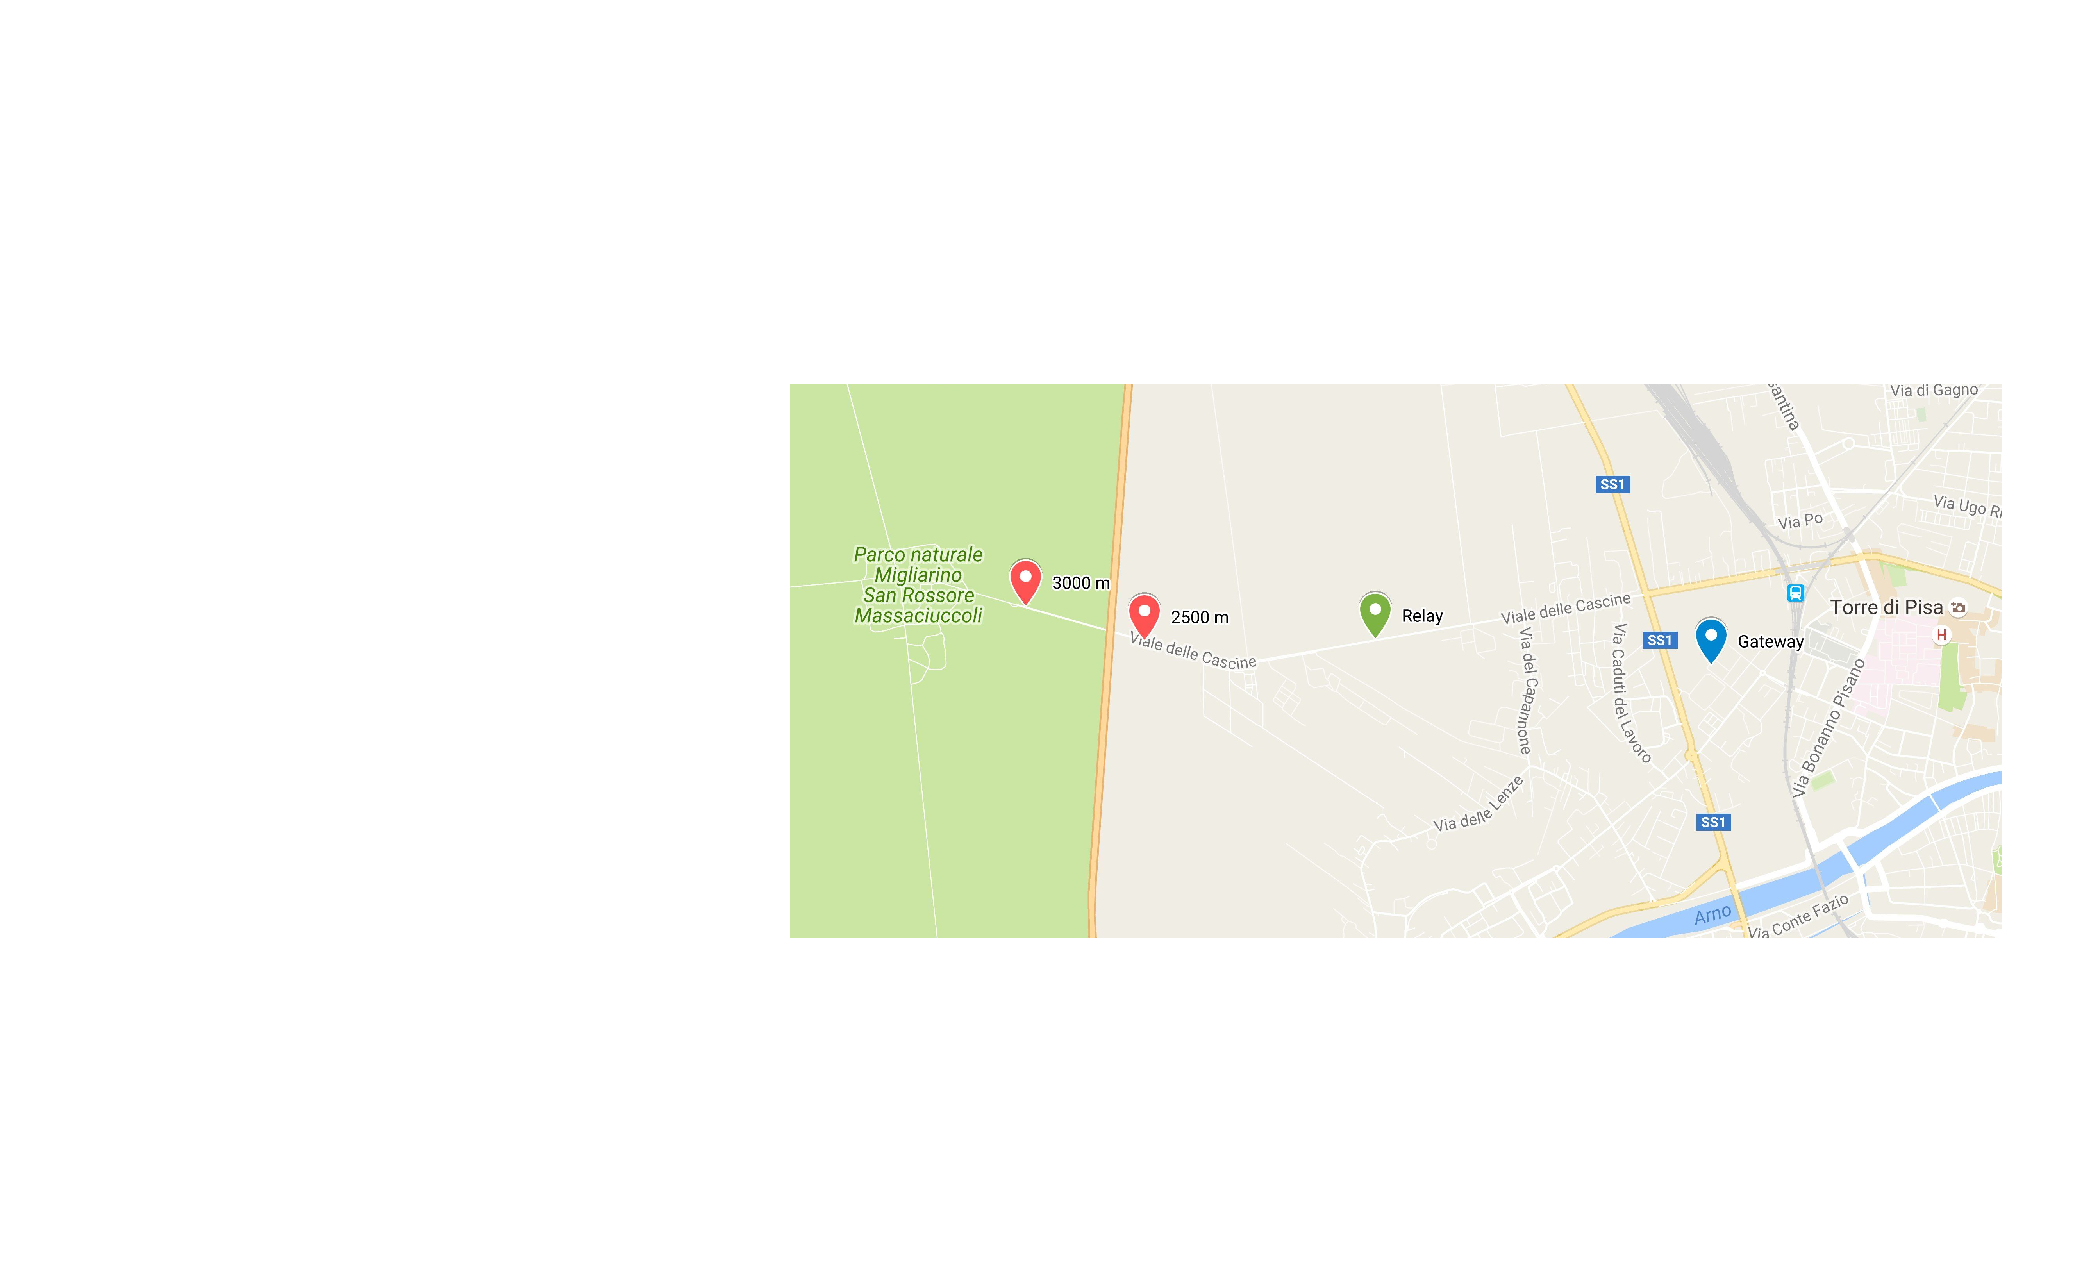
\includegraphics[width=\textwidth]{img/map_relay}
\caption{Map of rural experiments with relay}
\label{fig:maprelay}
\end{figure}

% Please add the following required packages to your document preamble:
% \usepackage{booktabs}
\begin{table}[]
\centering
\caption{Test configurations}
\label{tab:relay_test}
\begin{tabular}{@{}lll@{}}
\toprule
Parameter           & Values & Unit  \\ \midrule
Spreading factor    & 7, 10  &       \\
Transmission power  & 14, 8  & dBm   \\
Payload length      & 10, 50 & bytes \\
Distance from relay & 1, 1.5 & Km    \\ \bottomrule
\end{tabular}
\end{table}

\section{Results}
The results of the experiments, in general, were encouraging, since at 2500 meters from the gateway it was achieved a very low packet error rate combined to the reduction of transmission power, which essentially was the purpose of developing the relay-based solution.

The other great results has been effectively enlarging the coverage area without compromising neither the number of correctly received packets, nor the data rate. In this section the results of the experiments are shown, organized by spreading factor.

\subsubsection{Spreading Factor 7}

SF 7 is, at the same time, the fastest and the less reliable data rate, so it is expected to be the lower bound on the number of correctly received packets. As shown in figure \ref{fig:sf7relay} at 2.5 km all configuration has a percentage of correctly received packets greater then 80\%,  which is a giant leap ahead from the nearly 0\% packets received at the same distance with the single hop scheme. The good performace are confirmed also at 3.0 Km, which was not tested in single-hop scheme, with almost 60\% of correctly received packets in the worst case. In table \ref{tab:cisf7relay} are reported the confidence intervals for each configuration.

\begin{figure}[]
\centering
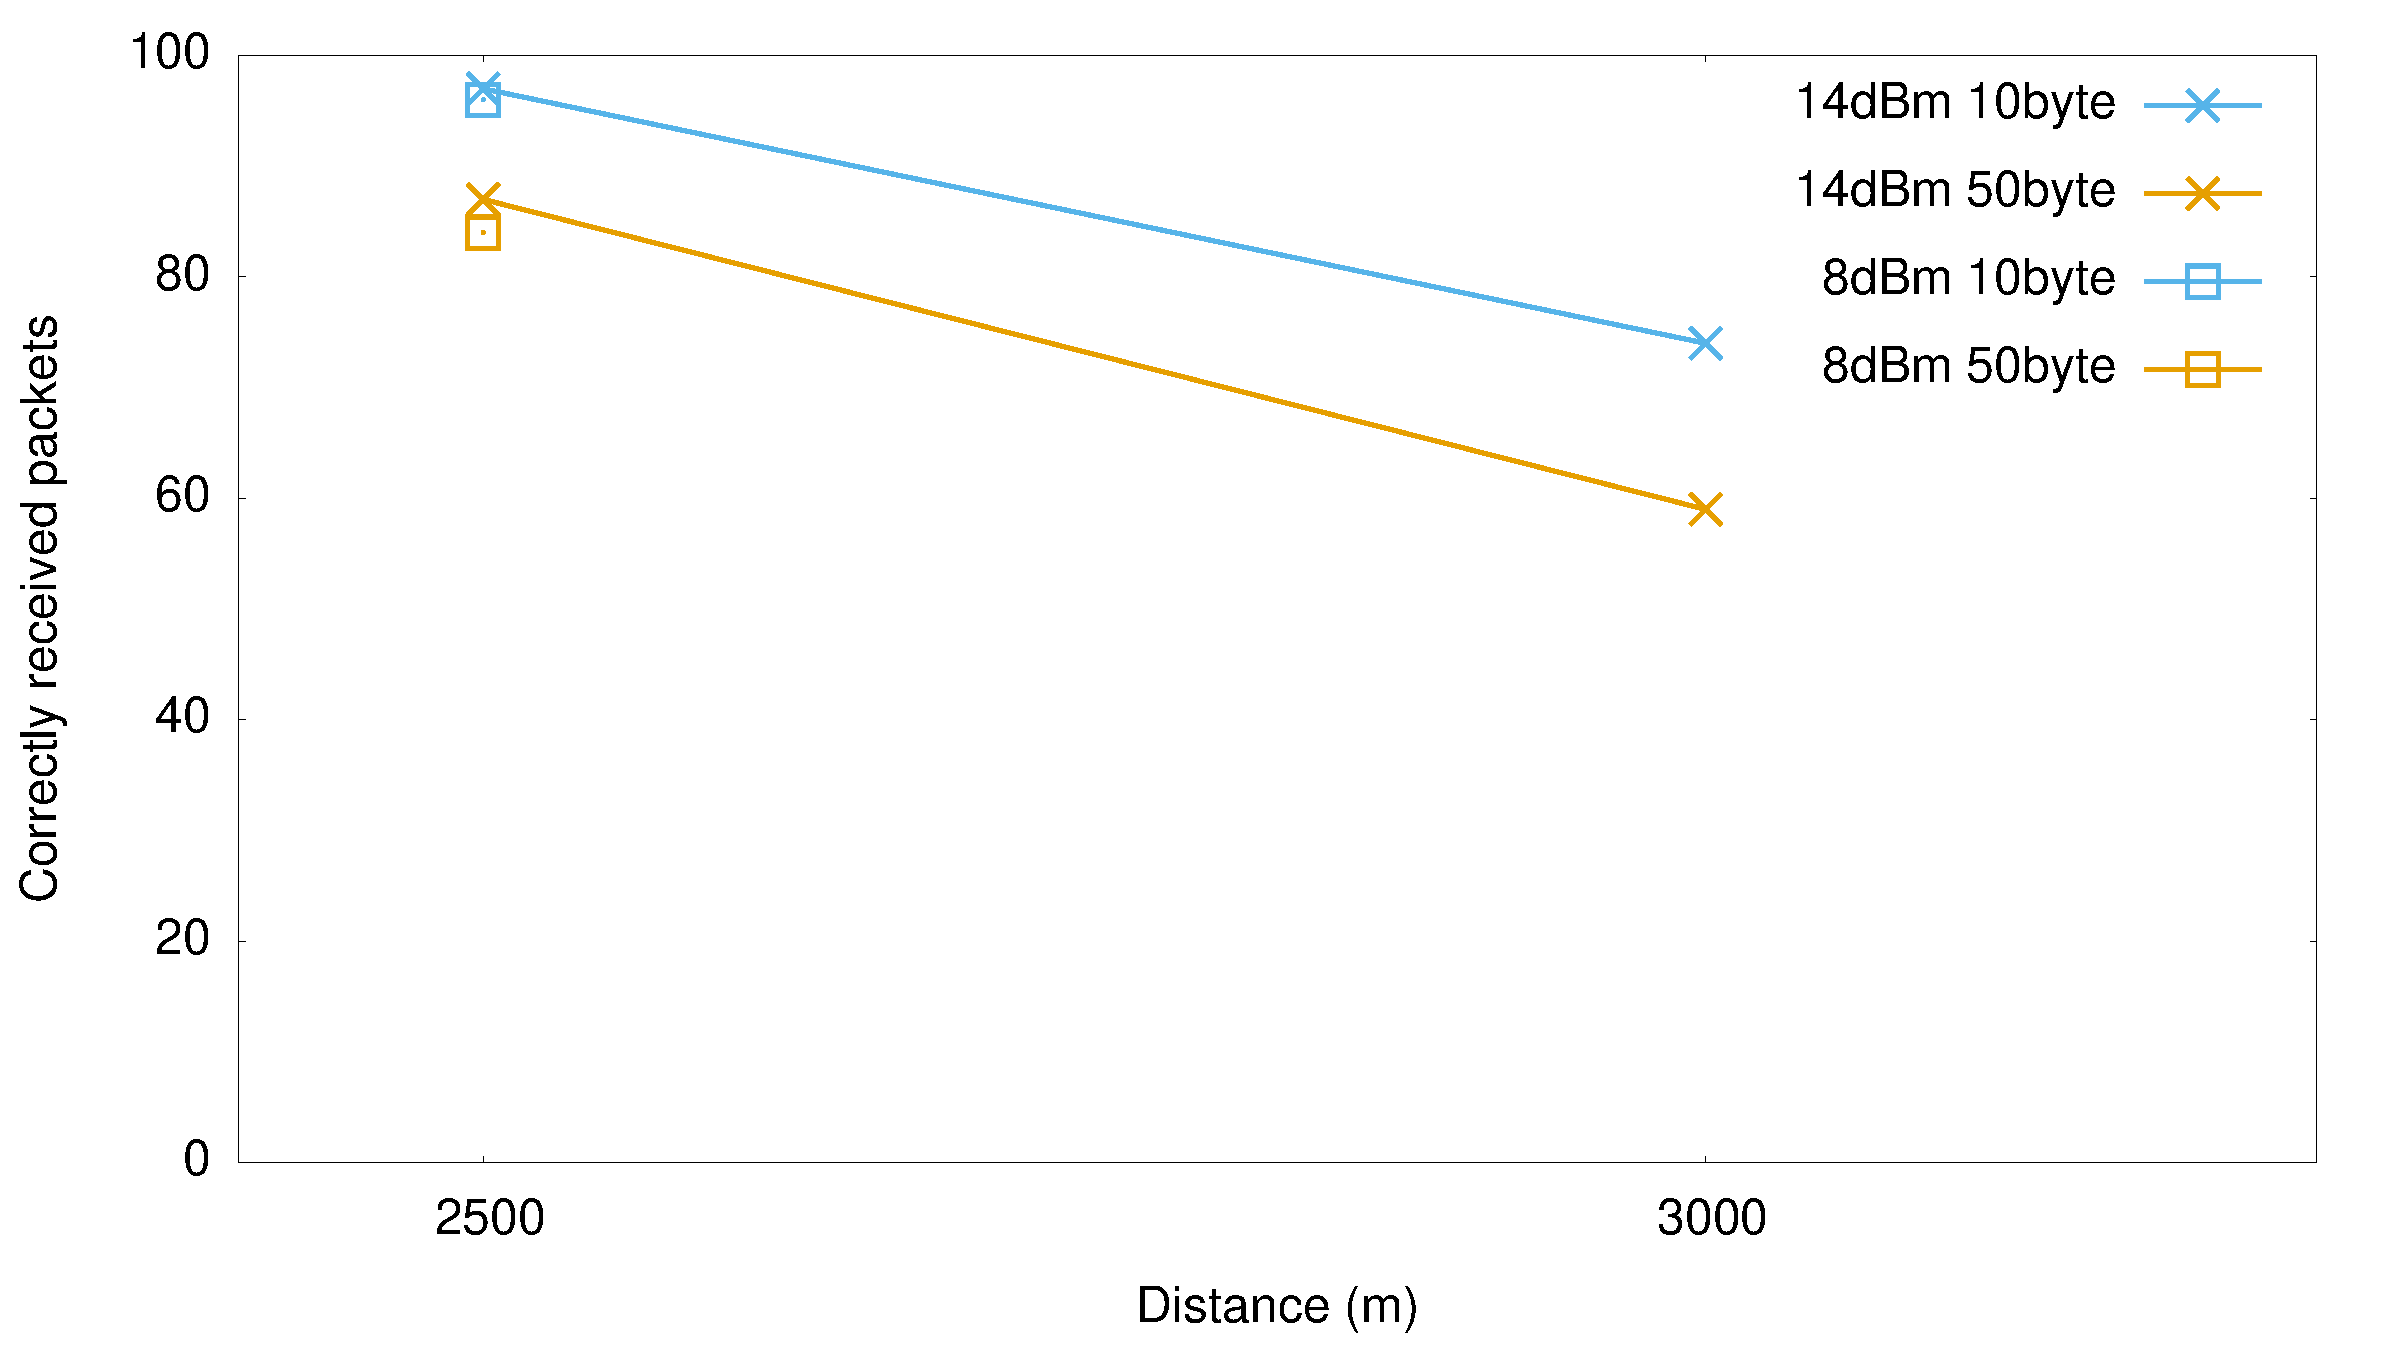
\includegraphics[width=\textwidth]{img/test/relay/sf7}
\caption{Results of two-hop experiments at SF 7}
\label{fig:sf7relay}
\end{figure}


\subsubsection{Spreading Factor 10}
SF 10 was expected to be more reliable, and in fact the results in figure \ref{fig:sf10relay} show even better performances than SF 7. At this data rate is possible to obtain up to 97\% of correctly received packets when considering 8 dBm as transmission power and 10 bytes as payload length.

Therefore this can be considered a remarkable achievement since the new two hop solution decreases both the packet error rate and the needed transmission power with basically no extra infrastructure needed. In table \ref{tab:cisf10relay} are reported the confidence intervals for each configuration. 

\begin{figure}[]
\centering
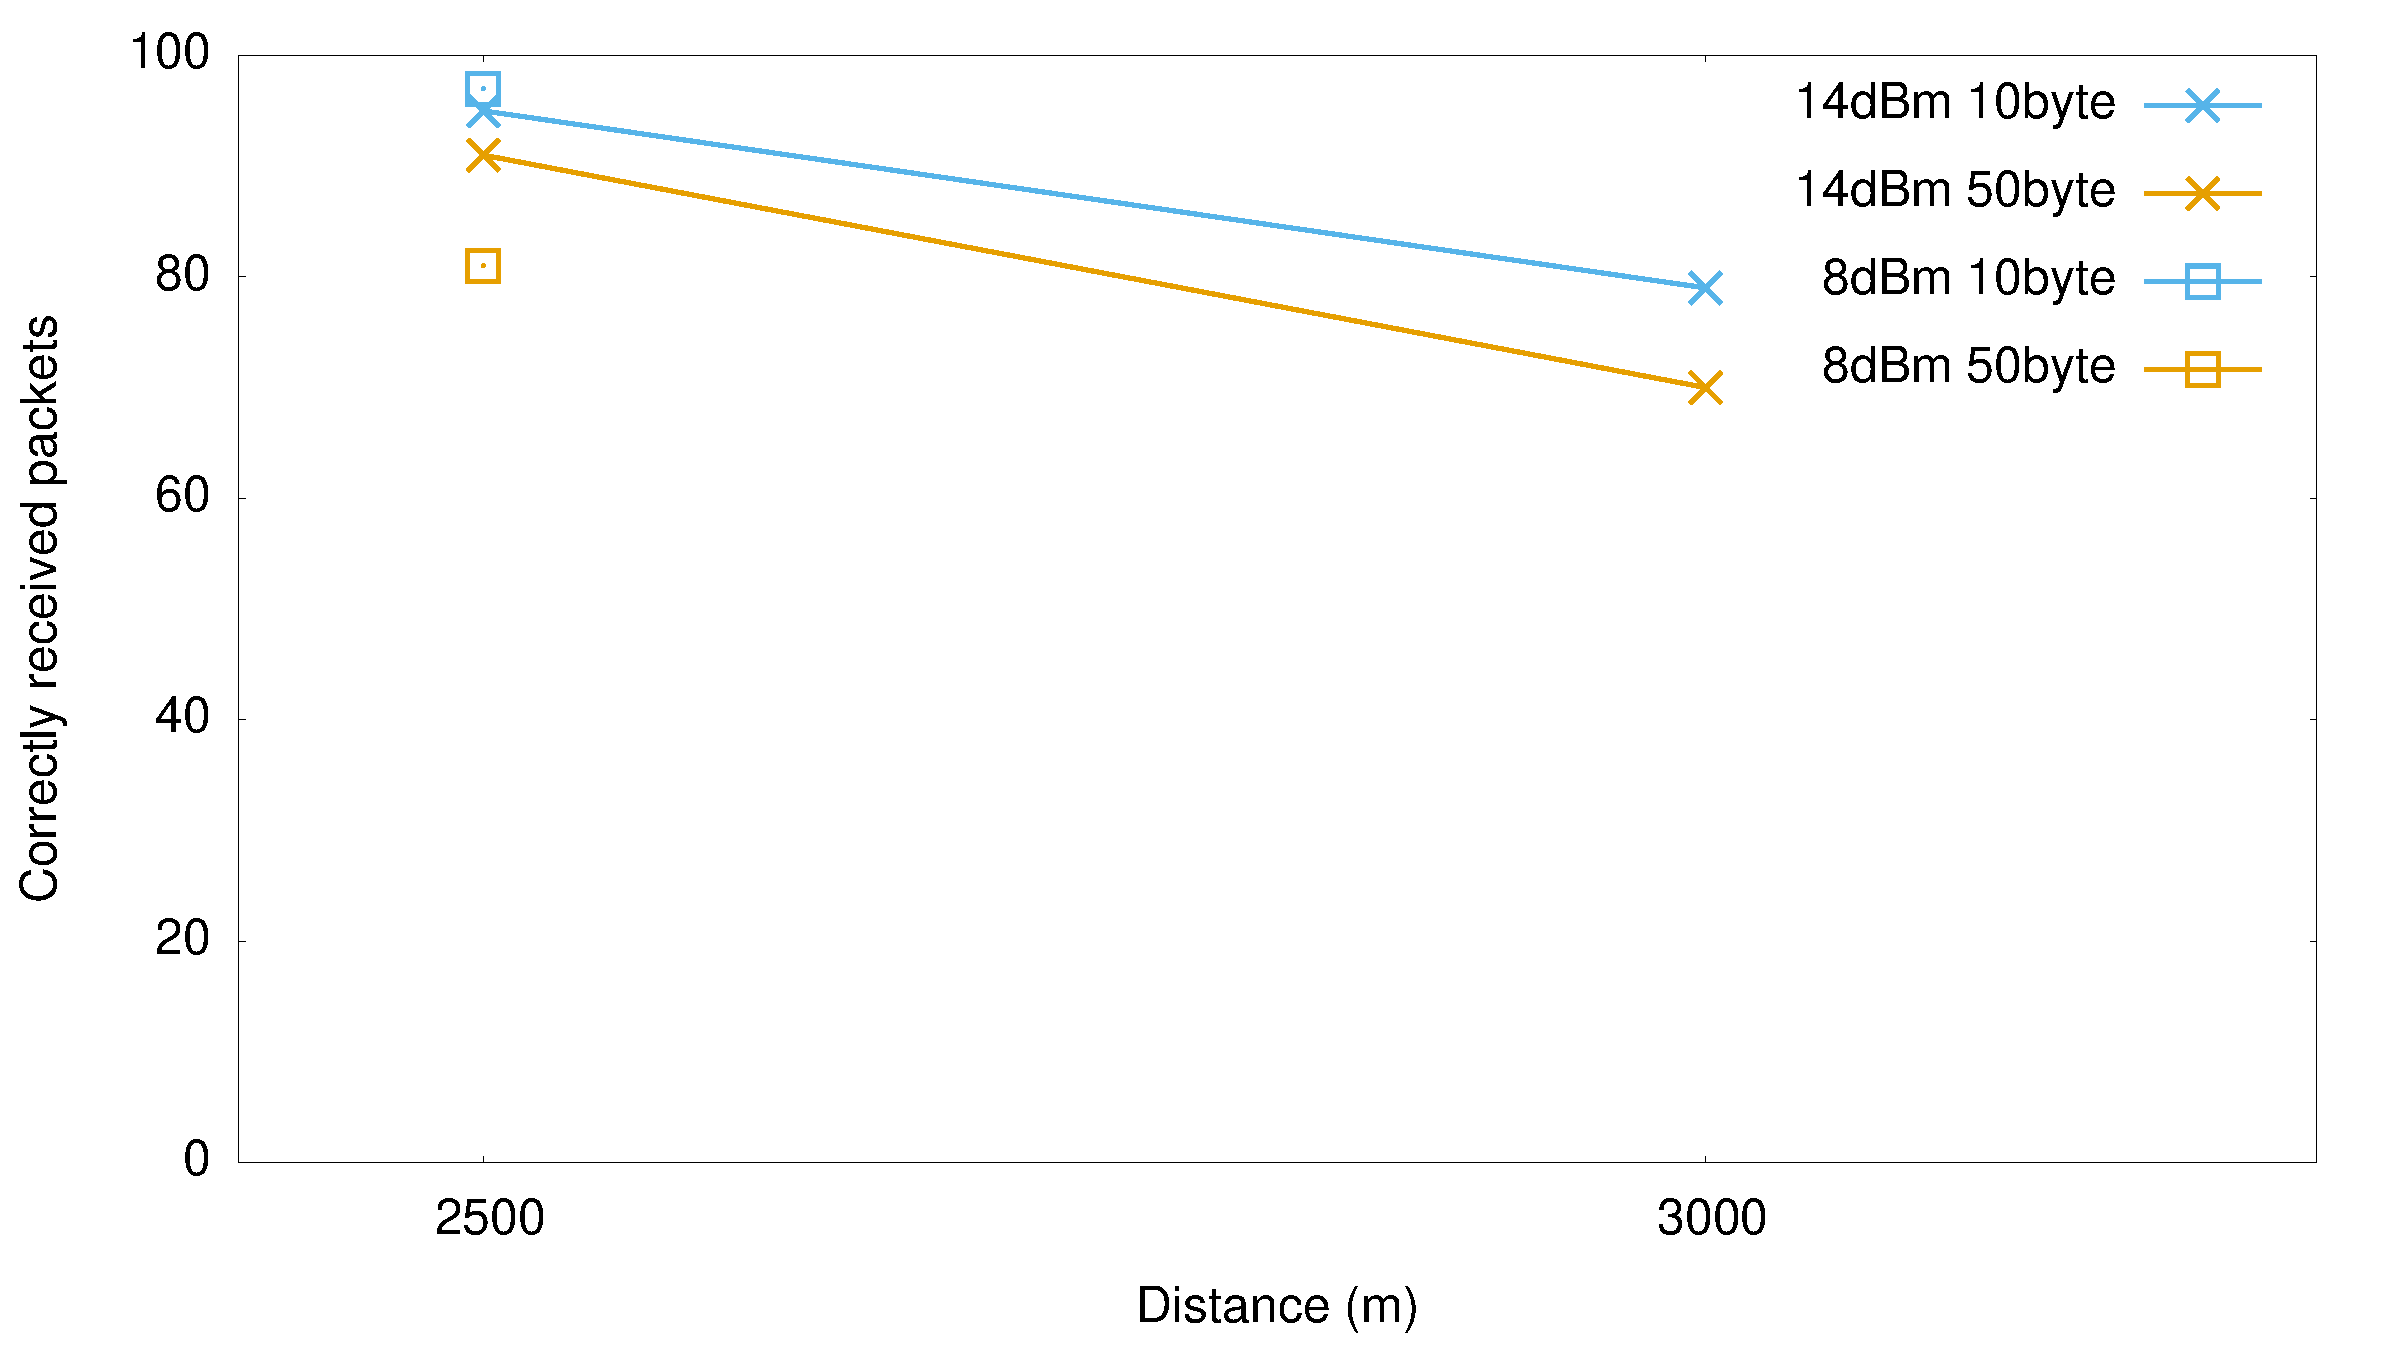
\includegraphics[width=\textwidth]{img/test/relay/sf10}
\caption{Results of two-hop experiments at SF 10}
\label{fig:sf10relay}
\end{figure}




\chapter{Conclusions}

In order to evaluate the performance of LoRaWAN a set of experiments was designed and conducted, using a custom implementation of the LoRa server infrastructure. As result of this operation it was discovered that the maximum possible distance that can be reach in rural area is 2500 meters, getting 71\% of correctly received packets using the most conservative (and slow) set-up (figure \ref{fig:sf12rural}). However the percentage falls at 14\% when considering higher data rate, SF10 in this case, and reach 0\% for the fastest data dates. The urban experiments, instead, showed results aligned to the theory, except for the influence of the forward error correction which in some cases were lower than expected.

Both from the results of a theoretical analysis, published in \cite{lorawanlimits}, and from the experimental data shown in chapter \ref{chap:experiments}, it has arisen the need to extend the LoRaWAN standards to support multi-hop communications using a relay-based solution.

The performances of the new architecture were evaluated through a set of experiments. Analyzing the results it turned out that at 2500 meters from the gateway it is possible to achieve up to 97\% of correctly received packets (10 bytes payload at SF 10, figure \ref{fig:sf10relay}), in comparison to only 14\% of correctly received packets with the standard one-hop topology in the same configuration (figure \ref{fig:sf10rural}). Moreover the two-hop solutions allowed to place the end-devices even further than the first set of experiments, reaching 79\% of correctly received packets at 3000 meters.

Therefore, it is possible to conclude that the proposed solution can drastically improve the reliability of the communication, preserving the features of LoRaWAN in terms of energy efficiency. Furthermore, thanks to this extension it is possible to effectively enlarge the coverage area of a LoRaWAN network without requiring the installation of new expensive gateways.

\section{Future development}
This work can be the starting point for future extensions, such as:

\begin{itemize}
\item Develop an efficient \emph{Network Controller} that can be integrated with LoRa server developed in this thesis.

\item Conduct some long-term experiments in order to collect more data and explore other possible scenarios in which it is reasonable to deploy the LoRaWAN technology.

\item Try to achieve a complete implementation of the relay protocol, overcoming the limits that have forced to develop a subset of the original specification.
\end{itemize}

\appendix
\chapter{Confidence intervals}
In this appendix the computed confidence intervals for the experiments are reported.

\newpage
\section{Rural experiments}
% Please add the following required packages to your document preamble:
% \usepackage{booktabs}
\begin{table}[H]
\centering
\caption{95\% confidence intervals at 500 meters}
\begin{tabular}{@{}ccccccc@{}}
\toprule
SF & \begin{tabular}[c]{@{}c@{}}Power\\ (dBm)\end{tabular} & \begin{tabular}[c]{@{}c@{}}Payload\\ (bytes)\end{tabular} & TX  & RX  & \multicolumn{2}{c}{Interval} \\ \midrule
7  & 8                                                     & 10                                                        & 100 & 100 & 1,0000        & 1,0000       \\
8  & 8                                                     & 10                                                        & 100 & 100 & 1,0000        & 1,0000       \\
9  & 8                                                     & 10                                                        & 100 & 100 & 1,0000        & 1,0000       \\
10 & 8                                                     & 10                                                        & 100 & 100 & 1,0000        & 1,0000       \\
11 & 8                                                     & 10                                                        & 100 & 97  & 0,9366        & 1,0000       \\
12 & 8                                                     & 10                                                        & 100 & 54  & 0,4423        & 0,6377       \\
7  & 8                                                     & 50                                                        & 100 & 99  & 0,9705        & 1,0000       \\
8  & 8                                                     & 50                                                        & 100 & 100 & 1,0000        & 1,0000       \\
9  & 8                                                     & 50                                                        & 100 & 99  & 0,9705        & 1,0000       \\
10 & 8                                                     & 50                                                        & 100 & 100 & 1,0000        & 1,0000       \\
11 & 8                                                     & 50                                                        & 100 & 98  & 0,9526        & 1,0000       \\
12 & 8                                                     & 50                                                        & 100 & 56  & 0,4627        & 0,6573       \\
7  & 2                                                     & 10                                                        & 100 & 99  & 0,9705        & 1,0000       \\
8  & 2                                                     & 10                                                        & 100 & 100 & 1,0000        & 1,0000       \\
9  & 2                                                     & 10                                                        & 100 & 99  & 0,9705        & 1,0000       \\
10 & 2                                                     & 10                                                        & 100 & 100 & 1,0000        & 1,0000       \\
11 & 2                                                     & 10                                                        & 100 & 99  & 0,9705        & 1,0000       \\
12 & 2                                                     & 10                                                        & 100 & 75  & 0,6651        & 0,8349       \\
7  & 2                                                     & 50                                                        & 100 & 100 & 1,0000        & 1,0000       \\
8  & 2                                                     & 50                                                        & 100 & 99  & 0,9705        & 1,0000       \\
9  & 2                                                     & 50                                                        & 100 & 100 & 1,0000        & 1,0000       \\
10 & 2                                                     & 50                                                        & 100 & 100 & 1,0000        & 1,0000       \\
11 & 2                                                     & 50                                                        & 100 & 98  & 0,9526        & 1,0000       \\
12 & 2                                                     & 50                                                        & 100 & 68  & 0,5886        & 0,7714       \\ \bottomrule
\end{tabular}
\end{table}


% Please add the following required packages to your document preamble:
% \usepackage{booktabs}
\begin{table}[H]
\centering
\caption{95\% confidence intervals at 1000 meters}
\begin{tabular}{@{}ccccccc@{}}
\toprule
SF & \begin{tabular}[c]{@{}c@{}}Power\\ (dBm)\end{tabular} & \begin{tabular}[c]{@{}c@{}}Payload\\ (bytes)\end{tabular} & TX  & RX  & \multicolumn{2}{c}{Interval} \\ \midrule
7  & 14                                                    & 10                                                        & 100 & 99  & 0,9705        & 1,0000       \\
8  & 14                                                    & 10                                                        & 100 & 100 & 1,0000        & 1,0000       \\
9  & 14                                                    & 10                                                        & 100 & 98  & 0,9526        & 1,0000       \\
10 & 14                                                    & 10                                                        & 100 & 100 & 1,0000        & 1,0000       \\
11 & 14                                                    & 10                                                        & 100 & 100 & 1,0000        & 1,0000       \\
12 & 14                                                    & 10                                                        & 100 & 97  & 0,9366        & 1,0000       \\
7  & 14                                                    & 50                                                        & 100 & 98  & 0,9526        & 1,0000       \\
8  & 14                                                    & 50                                                        & 100 & 100 & 1,0000        & 1,0000       \\
9  & 14                                                    & 50                                                        & 100 & 97  & 0,9366        & 1,0000       \\
10 & 14                                                    & 50                                                        & 100 & 100 & 1,0000        & 1,0000       \\
11 & 14                                                    & 50                                                        & 100 & 100 & 1,0000        & 1,0000       \\
12 & 14                                                    & 50                                                        & 100 & 95  & 0,9073        & 0,9927       \\
7  & 5                                                     & 10                                                        & 100 & 78  & 0,6988        & 0,8612       \\
8  & 5                                                     & 10                                                        & 100 & 92  & 0,8668        & 0,9732       \\
9  & 5                                                     & 10                                                        & 100 & 96  & 0,9216        & 0,9984       \\
10 & 5                                                     & 10                                                        & 100 & 96  & 0,9216        & 0,9984       \\
11 & 5                                                     & 10                                                        & 100 & 100 & 1,0000        & 1,0000       \\
12 & 5                                                     & 10                                                        & 100 & 99  & 0,9705        & 1,0000       \\
7  & 5                                                     & 50                                                        & 100 & 50  & 0,4020        & 0,5980       \\
8  & 5                                                     & 50                                                        & 100 & 79  & 0,7102        & 0,8698       \\
9  & 5                                                     & 50                                                        & 100 & 87  & 0,8041        & 0,9359       \\
10 & 5                                                     & 50                                                        & 100 & 93  & 0,8800        & 0,9800       \\
11 & 5                                                     & 50                                                        & 100 & 99  & 0,9705        & 1,0000       \\
12 & 5                                                     & 50                                                        & 100 & 98  & 0,9526        & 1,0000       \\ \bottomrule
\end{tabular}
\end{table}


\begin{table}[H]
\centering
\caption{95\% confidence intervals at 1500 meters}
\begin{tabular}{@{}ccccccc@{}}
\toprule
SF & \begin{tabular}[c]{@{}c@{}}Power\\ (dBm)\end{tabular} & \begin{tabular}[c]{@{}c@{}}Payload\\ (bytes)\end{tabular} & TX  & RX  & \multicolumn{2}{c}{Interval} \\ \midrule
7  & 14                                                    & 10                                                        & 100 & 100 & 1,0000        & 1,0000       \\
8  & 14                                                    & 10                                                        & 100 & 100 & 1,0000        & 1,0000       \\
9  & 14                                                    & 10                                                        & 100 & 99  & 0,9705        & 1,0000       \\
10 & 14                                                    & 10                                                        & 100 & 100 & 1,0000        & 1,0000       \\
11 & 14                                                    & 10                                                        & 100 & 100 & 1,0000        & 1,0000       \\
12 & 14                                                    & 10                                                        & 100 & 97  & 0,9366        & 1,0000       \\
7  & 14                                                    & 50                                                        & 100 & 97  & 0,9366        & 1,0000       \\
8  & 14                                                    & 50                                                        & 100 & 74  & 0,6540        & 0,8260       \\
9  & 14                                                    & 50                                                        & 100 & 99  & 0,9705        & 1,0000       \\
10 & 14                                                    & 50                                                        & 100 & 100 & 1,0000        & 1,0000       \\
11 & 14                                                    & 50                                                        & 100 & 100 & 1,0000        & 1,0000       \\
12 & 14                                                    & 50                                                        & 100 & 98  & 0,9526        & 1,0000       \\
7  & 8                                                     & 10                                                        & 100 & 91  & 0,8539        & 0,9661       \\
8  & 8                                                     & 10                                                        & 100 & 96  & 0,9216        & 0,9984       \\
9  & 8                                                     & 10                                                        & 100 & 100 & 1,0000        & 1,0000       \\
10 & 8                                                     & 10                                                        & 100 & 98  & 0,9526        & 1,0000       \\
11 & 8                                                     & 10                                                        & 100 & 100 & 1,0000        & 1,0000       \\
12 & 8                                                     & 10                                                        & 100 & 97  & 0,9366        & 1,0000       \\
7  & 8                                                     & 50                                                        & 100 & 86  & 0,7920        & 0,9280       \\
8  & 8                                                     & 50                                                        & 100 & 93  & 0,8800        & 0,9800       \\
9  & 8                                                     & 50                                                        & 100 & 99  & 0,9705        & 1,0000       \\
10 & 8                                                     & 50                                                        & 100 & 100 & 1,0000        & 1,0000       \\
11 & 8                                                     & 50                                                        & 100 & 98  & 0,9526        & 1,0000       \\
12 & 8                                                     & 50                                                        & 100 & 99  & 0,9705        & 1,0000       \\ \bottomrule
\end{tabular}
\end{table}


% Please add the following required packages to your document preamble:
% \usepackage{booktabs}
\begin{table}[H]
\centering
\caption{95\% confidence intervals at 2000 meters}
\begin{tabular}{@{}ccccccc@{}}
\toprule
SF & \begin{tabular}[c]{@{}c@{}}Power\\ (dBm)\end{tabular} & \begin{tabular}[c]{@{}c@{}}Payload\\ (bytes)\end{tabular} & TX  & RX & \multicolumn{2}{c}{Interval} \\ \midrule
7  & 14                                                    & 10                                                        & 100 & 10 & 0,0412        & 0,1588       \\
8  & 14                                                    & 10                                                        & 100 & 28 & 0,1920        & 0,3680       \\
9  & 14                                                    & 10                                                        & 100 & 48 & 0,3821        & 0,5779       \\
10 & 14                                                    & 10                                                        & 100 & 63 & 0,5354        & 0,7246       \\
11 & 14                                                    & 10                                                        & 100 & 72 & 0,6320        & 0,8080       \\
12 & 14                                                    & 10                                                        & 100 & 79 & 0,7102        & 0,8698       \\
7  & 14                                                    & 50                                                        & 100 & 2  & 0,0000        & 0,0474       \\
8  & 14                                                    & 50                                                        & 100 & 19 & 0,1131        & 0,2669       \\
9  & 14                                                    & 50                                                        & 100 & 35 & 0,2565        & 0,4435       \\
10 & 14                                                    & 50                                                        & 100 & 56 & 0,4627        & 0,6573       \\
11 & 14                                                    & 50                                                        & 100 & 64 & 0,5459        & 0,7341       \\
12 & 14                                                    & 50                                                        & 100 & 76 & 0,6763        & 0,8437       \\
7  & 8                                                     & 10                                                        & 100 & 0  & 0,0000        & 0,0000       \\
8  & 8                                                     & 10                                                        & 100 & 0  & 0,0000        & 0,0000       \\
9  & 8                                                     & 10                                                        & 100 & 3  & 0,0000        & 0,0634       \\
10 & 8                                                     & 10                                                        & 100 & 17 & 0,0964        & 0,2436       \\
11 & 8                                                     & 10                                                        & 100 & 43 & 0,3330        & 0,5270       \\
12 & 8                                                     & 10                                                        & 100 & 54 & 0,4423        & 0,6377       \\
7  & 8                                                     & 50                                                        & 100 & 0  & 0,0000        & 0,0000       \\
8  & 8                                                     & 50                                                        & 100 & 0  & 0,0000        & 0,0000       \\
9  & 8                                                     & 50                                                        & 100 & 5  & 0,0073        & 0,0927       \\
10 & 8                                                     & 50                                                        & 100 & 8  & 0,0268        & 0,1332       \\
11 & 8                                                     & 50                                                        & 100 & 28 & 0,1920        & 0,3680       \\
12 & 8                                                     & 50                                                        & 100 & 46 & 0,3623        & 0,5577       \\ \bottomrule
\end{tabular}
\end{table}




\begin{table}[H]
\centering
\caption{95\% confidence intervals at 2500 meters}
\begin{tabular}{@{}ccccccc@{}}
\toprule
SF & \begin{tabular}[c]{@{}c@{}}Power\\ (dBm)\end{tabular} & \begin{tabular}[c]{@{}c@{}}Payload\\ (bytes)\end{tabular} & TX  & RX & \multicolumn{2}{c}{Interval} \\ \midrule
7  & 14                                                    & 10                                                        & 100 & 0  & 0,0000        & 0,0000       \\
8  & 14                                                    & 10                                                        & 100 & 7  & 0,0200        & 0,1200       \\
9  & 14                                                    & 10                                                        & 100 & 25 & 0,1651        & 0,3349       \\
10 & 14                                                    & 10                                                        & 100 & 14 & 0,0720        & 0,2080       \\
11 & 14                                                    & 10                                                        & 100 & 64 & 0,5459        & 0,7341       \\
12 & 14                                                    & 10                                                        & 100 & 71 & 0,6211        & 0,7989       \\
7  & 14                                                    & 50                                                        & 100 & 0  & 0,0000        & 0,0000       \\
8  & 14                                                    & 50                                                        & 100 & 0  & 0,0000        & 0,0000       \\
9  & 14                                                    & 50                                                        & 100 & 2  & 0,0000        & 0,0474       \\
10 & 14                                                    & 50                                                        & 100 & 7  & 0,0200        & 0,1200       \\
11 & 14                                                    & 50                                                        & 100 & 6  & 0,0135        & 0,1065       \\
12 & 14                                                    & 50                                                        & 100 & 27 & 0,1830        & 0,3570       \\
7  & 8                                                     & 10                                                        & 100 & 0  & 0,0000        & 0,0000       \\
8  & 8                                                     & 10                                                        & 100 & 0  & 0,0000        & 0,0000       \\
9  & 8                                                     & 10                                                        & 100 & 0  & 0,0000        & 0,0000       \\
10 & 8                                                     & 10                                                        & 100 & 0  & 0,0000        & 0,0000       \\
11 & 8                                                     & 10                                                        & 100 & 2  & 0,0000        & 0,0474       \\
12 & 8                                                     & 10                                                        & 100 & 10 & 0,0412        & 0,1588       \\
7  & 8                                                     & 50                                                        & 100 & 0  & 0,0000        & 0,0000       \\
8  & 8                                                     & 50                                                        & 100 & 0  & 0,0000        & 0,0000       \\
9  & 8                                                     & 50                                                        & 100 & 0  & 0,0000        & 0,0000       \\
10 & 8                                                     & 50                                                        & 100 & 0  & 0,0000        & 0,0000       \\
11 & 8                                                     & 50                                                        & 100 & 0  & 0,0000        & 0,0000       \\
12 & 8                                                     & 50                                                        & 100 & 1  & 0,0000        & 0,0295       \\ \bottomrule
\end{tabular}
\end{table}




\newpage
\section{Urban experiments}
% Please add the following required packages to your document preamble:
% \usepackage{booktabs}
\begin{table}[H]
\centering
\caption{95\% confidence interval at SF 7}
\begin{tabular}{@{}ccccccc@{}}
\toprule
\begin{tabular}[c]{@{}c@{}}Power\\ (dBm)\end{tabular} & \begin{tabular}[c]{@{}c@{}}Payload\\ (bytes)\end{tabular} & CR  & TX  & RX & \multicolumn{2}{c}{Interval} \\ \midrule
2                                                     & 10                                                        & 4/5 & 100 & 0  & 0,0000        & 0,0000       \\
2                                                     & 10                                                        & 4/8 & 100 & 0  & 0,0000        & 0,0000       \\
2                                                     & 50                                                        & 4/5 & 100 & 0  & 0,0000        & 0,0000       \\
2                                                     & 50                                                        & 4/8 & 100 & 0  & 0,0000        & 0,0000       \\
5                                                     & 10                                                        & 4/5 & 100 & 12 & 0,0563        & 0,1837       \\
5                                                     & 10                                                        & 4/8 & 100 & 25 & 0,1651        & 0,3349       \\
5                                                     & 50                                                        & 4/5 & 100 & 0  & 0,0000        & 0,0000       \\
5                                                     & 50                                                        & 4/8 & 100 & 0  & 0,0000        & 0,0000       \\
8                                                     & 10                                                        & 4/5 & 100 & 86 & 0,7920        & 0,9280       \\
8                                                     & 10                                                        & 4/8 & 100 & 93 & 0,8800        & 0,9800       \\
8                                                     & 50                                                        & 4/5 & 100 & 0  & 0,0000        & 0,0000       \\
8                                                     & 50                                                        & 4/8 & 100 & 0  & 0,0000        & 0,0000       \\
14                                                    & 10                                                        & 4/5 & 100 & 98 & 0,9526        & 1,0000       \\
14                                                    & 10                                                        & 4/8 & 100 & 99 & 0,9705        & 1,0000       \\
14                                                    & 50                                                        & 4/5 & 100 & 87 & 0,8041        & 0,9359       \\
14                                                    & 50                                                        & 4/8 & 100 & 95 & 0,9073        & 0,9927       \\ \bottomrule
\end{tabular}
\end{table}


\begin{table}[H]
\centering
\caption{95\% confidence interval at SF 8}
\begin{tabular}{ccccccc}
\toprule
\begin{tabular}[c]{@{}c@{}}Power\\ (dBm)\end{tabular} & \begin{tabular}[c]{@{}c@{}}Payload\\ (bytes)\end{tabular} & CR  & TX  & RX  & \multicolumn{2}{c}{Interval} \\
\midrule
2                                                     & 10                                                        & 4/5 & 100 & 3   & 0,0000        & 0,0634       \\
2                                                     & 10                                                        & 4/8 & 100 & 22  & 0,1388        & 0,3012       \\
2                                                     & 50                                                        & 4/5 & 100 & 0   & 0,0000        & 0,0000       \\
2                                                     & 50                                                        & 4/8 & 100 & 0   & 0,0000        & 0,0000       \\
5                                                     & 10                                                        & 4/5 & 100 & 77  & 0,6875        & 0,8525       \\
5                                                     & 10                                                        & 4/8 & 100 & 87  & 0,8041        & 0,9359       \\
5                                                     & 50                                                        & 4/5 & 100 & 0   & 0,0000        & 0,0000       \\
5                                                     & 50                                                        & 4/8 & 100 & 0   & 0,0000        & 0,0000       \\
8                                                     & 10                                                        & 4/5 & 100 & 95  & 0,9073        & 0,9927       \\
8                                                     & 10                                                        & 4/8 & 100 & 99  & 0,9705        & 1,0000       \\
8                                                     & 50                                                        & 4/5 & 100 & 5   & 0,0073        & 0,0927       \\
8                                                     & 50                                                        & 4/8 & 100 & 3   & 0,0000        & 0,0634       \\
14                                                    & 10                                                        & 4/5 & 100 & 96  & 0,9216        & 0,9984       \\
14                                                    & 10                                                        & 4/8 & 100 & 100 & 1,0000        & 1,0000       \\
14                                                    & 50                                                        & 4/5 & 100 & 96  & 0,9216        & 0,9984       \\
14                                                    & 50                                                        & 4/8 & 100 & 97  & 0,9366        & 1,0000      \\ \bottomrule
\end{tabular}
\end{table}



% Please add the following required packages to your document preamble:
% \usepackage{booktabs}
\begin{table}[H]
\centering
\caption{95\% confidence interval at SF 9}
\begin{tabular}{@{}ccccccc@{}}
\toprule
\begin{tabular}[c]{@{}c@{}}Power\\ (dBm)\end{tabular} & \begin{tabular}[c]{@{}c@{}}Payload\\ (bytes)\end{tabular} & CR  & TX  & RX & \multicolumn{2}{c}{Interval} \\ \midrule
2                                                     & 10                                                        & 4/5 & 100 & 82 & 0,7447        & 0,8953       \\
2                                                     & 10                                                        & 4/8 & 100 & 95 & 0,9073        & 0,9927       \\
2                                                     & 50                                                        & 4/5 & 100 & 0  & 0,0000        & 0,0000       \\
2                                                     & 50                                                        & 4/8 & 100 & 0  & 0,0000        & 0,0000       \\
5                                                     & 10                                                        & 4/5 & 100 & 93 & 0,8800        & 0,9800       \\
5                                                     & 10                                                        & 4/8 & 100 & 97 & 0,9366        & 1,0000       \\
5                                                     & 50                                                        & 4/5 & 100 & 4  & 0,0016        & 0,0784       \\
5                                                     & 50                                                        & 4/8 & 100 & 43 & 0,3330        & 0,5270       \\
8                                                     & 10                                                        & 4/5 & 100 & 96 & 0,9216        & 0,9984       \\
8                                                     & 10                                                        & 4/8 & 100 & 99 & 0,9705        & 1,0000       \\
8                                                     & 50                                                        & 4/5 & 100 & 78 & 0,6988        & 0,8612       \\
8                                                     & 50                                                        & 4/8 & 100 & 92 & 0,8668        & 0,9732       \\
14                                                    & 10                                                        & 4/5 & 100 & 99 & 0,9705        & 1,0000       \\
14                                                    & 10                                                        & 4/8 & 100 & 99 & 0,9705        & 1,0000       \\
14                                                    & 50                                                        & 4/5 & 100 & 96 & 0,9216        & 0,9984       \\
14                                                    & 50                                                        & 4/8 & 100 & 99 & 0,9705        & 1,0000       \\ \bottomrule
\end{tabular}
\end{table}




% Please add the following required packages to your document preamble:
% \usepackage{booktabs}
\begin{table}[H]
\centering
\caption{95\% confidence interval at SF 10}
\begin{tabular}{@{}ccccccc@{}}
\toprule
\begin{tabular}[c]{@{}c@{}}Power\\ (dBm)\end{tabular} & \begin{tabular}[c]{@{}c@{}}Payload\\ (bytes)\end{tabular} & CR  & TX  & RX  & \multicolumn{2}{c}{Interval} \\ \midrule
2     & 10      & 4/5 & 100 & 94  & 0,8935        & 0,9865       \\
2     & 10      & 4/8 & 100 & 97  & 0,9366        & 1,0000       \\
2     & 50      & 4/5 & 100 & 1   & 0,0000        & 0,0295       \\
2     & 50      & 4/8 & 100 & 37  & 0,2754        & 0,4646       \\
5     & 10      & 4/5 & 100 & 100 & 1,0000        & 1,0000       \\
5     & 10      & 4/8 & 100 & 99  & 0,9705        & 1,0000       \\
5     & 50      & 4/5 & 100 & 60  & 0,5040        & 0,6960       \\
5     & 50      & 4/8 & 100 & 88  & 0,8163        & 0,9437       \\
8     & 10      & 4/5 & 100 & 99  & 0,9705        & 1,0000       \\
8     & 10      & 4/8 & 100 & 99  & 0,9705        & 1,0000       \\
8     & 50      & 4/5 & 100 & 98  & 0,9526        & 1,0000       \\
8     & 50      & 4/8 & 100 & 99  & 0,9705        & 1,0000       \\
14    & 10      & 4/5 & 100 & 100 & 1,0000        & 1,0000       \\
14    & 10      & 4/8 & 100 & 100 & 1,0000        & 1,0000       \\
14    & 50      & 4/5 & 100 & 98  & 0,9526        & 1,0000       \\
14    & 50      & 4/8 & 100 & 100 & 1,0000        & 1,0000       \\ \bottomrule
\end{tabular}
\end{table}



% Please add the following required packages to your document preamble:
% \usepackage{booktabs}
\begin{table}[H]
\centering
\caption{95\% confidence interval at SF 11}
\begin{tabular}{@{}ccccccc@{}}
\toprule
\begin{tabular}[c]{@{}c@{}}Power\\ (dBm)\end{tabular} & \begin{tabular}[c]{@{}c@{}}Payload\\ (bytes)\end{tabular} & CR  & TX  & RX  & \multicolumn{2}{c}{Interval} \\ \midrule
2                                                     & 10                                                        & 4/5 & 100 & 95  & 0,9073        & 0,9927       \\
2                                                     & 10                                                        & 4/8 & 100 & 99  & 0,9705        & 1,0000       \\
2                                                     & 50                                                        & 4/5 & 100 & 51  & 0,4120        & 0,6080       \\
2                                                     & 50                                                        & 4/8 & 100 & 57  & 0,4730        & 0,6670       \\
5                                                     & 10                                                        & 4/5 & 100 & 97  & 0,9366        & 1,0000       \\
5                                                     & 10                                                        & 4/8 & 100 & 100 & 1,0000        & 1,0000       \\
5                                                     & 50                                                        & 4/5 & 100 & 85  & 0,7800        & 0,9200       \\
5                                                     & 50                                                        & 4/8 & 100 & 96  & 0,9216        & 0,9984       \\
8                                                     & 10                                                        & 4/5 & 100 & 100 & 1,0000        & 1,0000       \\
8                                                     & 10                                                        & 4/8 & 100 & 100 & 1,0000        & 1,0000       \\
8                                                     & 50                                                        & 4/5 & 100 & 99  & 0,9705        & 1,0000       \\
8                                                     & 50                                                        & 4/8 & 100 & 99  & 0,9705        & 1,0000       \\
14                                                    & 10                                                        & 4/5 & 100 & 100 & 1,0000        & 1,0000       \\
14                                                    & 10                                                        & 4/8 & 100 & 100 & 1,0000        & 1,0000       \\
14                                                    & 50                                                        & 4/5 & 100 & 98  & 0,9526        & 1,0000       \\
14                                                    & 50                                                        & 4/8 & 100 & 100 & 1,0000        & 1,0000       \\ \bottomrule
\end{tabular}
\end{table}


% Please add the following required packages to your document preamble:
% \usepackage{booktabs}
\begin{table}[H]
\centering
\caption{95\% confidence interval at SF 12}
\begin{tabular}{@{}ccccccc@{}}
\toprule
\begin{tabular}[c]{@{}c@{}}Power\\ (dBm)\end{tabular} & \begin{tabular}[c]{@{}c@{}}Payload\\ (bytes)\end{tabular} & CR  & TX  & RX  & \multicolumn{2}{c}{Interval} \\ \midrule
2                                                     & 10                                                        & 4/5 & 100 & 99  & 0,9705        & 1,0000       \\
2                                                     & 10                                                        & 4/8 & 100 & 97  & 0,9366        & 1,0000       \\
2                                                     & 50                                                        & 4/5 & 100 & 75  & 0,6651        & 0,8349       \\
2                                                     & 50                                                        & 4/8 & 100 & 82  & 0,7447        & 0,8953       \\
5                                                     & 10                                                        & 4/5 & 100 & 98  & 0,9526        & 1,0000       \\
5                                                     & 10                                                        & 4/8 & 100 & 99  & 0,9705        & 1,0000       \\
5                                                     & 50                                                        & 4/5 & 100 & 95  & 0,9073        & 0,9927       \\
5                                                     & 50                                                        & 4/8 & 100 & 97  & 0,9366        & 1,0000       \\
8                                                     & 10                                                        & 4/5 & 100 & 97  & 0,9366        & 1,0000       \\
8                                                     & 10                                                        & 4/8 & 100 & 98  & 0,9526        & 1,0000       \\
8                                                     & 50                                                        & 4/5 & 100 & 100 & 1,0000        & 1,0000       \\
8                                                     & 50                                                        & 4/8 & 100 & 99  & 0,9705        & 1,0000       \\
14                                                    & 10                                                        & 4/5 & 100 & 97  & 0,9366        & 1,0000       \\
14                                                    & 10                                                        & 4/8 & 100 & 97  & 0,9366        & 1,0000       \\
14                                                    & 50                                                        & 4/5 & 100 & 93  & 0,8800        & 0,9800       \\
14                                                    & 50                                                        & 4/8 & 100 & 99  & 0,9705        & 1,0000       \\ \bottomrule
\end{tabular}
\end{table}

\newpage
\section{Rural experiments with relay}

% Please add the following required packages to your document preamble:
% \usepackage{booktabs}
\begin{table}[H]
\centering
\caption{95\% confidence interval with relay at SF 7}
\label{tab:cisf7relay}
\begin{tabular}{@{}ccccccc@{}}
\toprule
Dist. (Km) & Power (dBm) & Payload (bytes) & TX  & RX & \multicolumn{2}{c}{Interval} \\ \midrule
2.5           & 14          & 10              & 100 & 70 & 0,6102        & 0,7898       \\
2.5           & 14          & 50              & 100 & 87 & 0,8041        & 0,9359       \\
2.5           & 8           & 10              & 100 & 47 & 0,3722        & 0,5678       \\
2.5           & 8           & 50              & 100 & 84 & 0,7681        & 0,9119       \\
3.0           & 14          & 10              & 100 & 74 & 0,6540        & 0,8260       \\
3.0          & 14          & 50              & 100 & 69 & 0,5994        & 0,7806       \\ \bottomrule
\end{tabular}
\end{table}

% Please add the following required packages to your document preamble:
% \usepackage{booktabs}
\begin{table}[H]
\centering
\caption{95\% confidence interval with relay at SF 10}
\label{tab:cisf10relay}
\begin{tabular}{@{}ccccccc@{}}
\toprule
Dist. (Km) & Power (dBm) & Payload (bytes) & TX  & RX & \multicolumn{2}{c}{Interval} \\ \midrule
2.5           & 14          & 10              & 100 & 90 & 0,8412        & 0,9588       \\
2.5           & 14          & 50              & 100 & 91 & 0,8539        & 0,9661       \\
2.5          & 8           & 10              & 100 & 97 & 0,9366        & 1,0000       \\
2.5           & 8           & 50              & 100 & 81 & 0,7331        & 0,8869       \\
3.0           & 14          & 10              & 100 & 79 & 0,7102        & 0,8698       \\
3.0           & 14          & 50              & 100 & 70 & 0,6102        & 0,7898       \\ \bottomrule
\end{tabular}
\end{table}


\bibliographystyle{plain} % stile bibliografia
\bibliography{thesis} % inserisce la bibliografia

\end{document}